\documentclass[letterpaper,11pt,leqno]{article}
\usepackage{paper}
\usepackage{placeins}
\bibliographystyle{bibliography}

% Enter title (to populate the PDF metadata):
\hypersetup{pdftitle={Paper Title}}

% Enter BibTeX file with references:
\newcommand{\bib}{bibliography}

% Enter PDF file with figures:
\newcommand{\pdf}{figures.pdf}

\begin{document}


% Enter title:
\title{Modern Versus Period Sausage Making}

% Enter authors:
\author{Daniel MacIver(Parker)
%
% Enter affiliations and acknowledgements:
\thanks{Daniel Parker: Middle Kingdom. I would like to thank my Laurel Rosamund for her support.}}

% I would also like to thank the multitude of laurels who helped source, review, and proofread for me.

% Enter date:
\date{May 2024}   

% Enter permanent URL (can be commented out):
%\available{https://github.com/pmichaillat/latex-paper}

\begin{titlepage}
\maketitle

% Enter abstract:
In this paper I discuss the differences in the tools and techniques for making sausage between modern and period (13th - 16th century in Western Europe specifically) techniques and tools. We will discuss the effects that the modern versus the period techniques had on the end product and if there were any significant differences in the taste or texture of the sausage. The same recipe will be used with the only differences being the techniques or tools.

\end{titlepage}

% Enter main text:
\section{Introduction}\label{s:introduction}
 
\paragraph{Background} The tools and techniques used for sausage making in period have not changed in a significant manner from the time of the Romans until we leave period late 1600s. The general process was to choose either a decently fatty meat or add in fat to more lean meat, chop and if needed pound the meat to the desired consistency, mix in salt and any other spices (usually during the chopping/beating process), and then stuff the mixture into some sort of casing (sometimes just forming it into shapes) which is usually made of some part of the digestive tract (intestines, stomach, bung, etc) though there are examples of other animals being used like the necks of different poultry.

Once the sausages were stuffed they would then either need to be cooked and eaten or preserved in some manner. There were many ways used to cook sausages in period. To cook the sausages they might boil them, fry in a pan, parboil then fry in a pan, hot smoke in the chimney, cook over a fire, simmer in soup, etc. The preservation methods were a little less varied but still very interesting. To preserve them they might cold smoke/dry them in the rafters, parboil them and leave to dry, sometimes go straight to hang drying, cover in honey or oils, salt cure them, etc.

Bacon in period was an interesting pork product. It did not generally match what we think of today as bacon. Bacon was a more general term for a salted/cured bit of either pork back or belly and was not usually smoked. It only started to be mentioned as possibly smoked at the very end of the 16th century. It was mentioned as purely salt cured and stored in salt like salt pork or removed after a period of time and hung in a cool dry area (much like today's pancetta).

The main focus of this research is on the Western European area in the 13th -- 16th centuries. The main reason that I am focusing on this time period is due to in the 13th century we start getting what are essentially the first modern cookbooks and the prevalence of them increases throughout the rest of the time period. 

 
\paragraph{Research Difficulties} Since some parts of the process were either fairly well known or a guild secret there are parts of this process which were not well documented. For example most recipes just say to "fill the casings" and don't elaborate on how the casings are supposed to be filled. This might be due to the indifference of the author on how the casings are filled. There are a couple different ways one might fill a casing with meat mixture. Making meatballs and stuffing those into the casing, manually stuffing the casing by hand, using a funnel to assist while having the casing fed onto the neck of the funnel, etc.

Another factor which is missing in pretty much every recipe that I have found was the water which needs to be added to allow the emulsion to form. There are a few hints here and there that such a thing was done based on some of the described textures after the mixing/beating process but it was also known to be one of the secrets of the sausage making guilds or families.

I went though over 40 different texts from English, French, and German to try and find references or resources to these different techniques but I was not able to find any clear examples where they directed the use of a funnel or any other specific method within this time period and region. There were one or two texts from Arabic regions where they describe the use of a funnel for stuffing a couple centuries before the western resources. We also know that there was a significant influence on Western European cookery books and cooks from first Roman texts but also some later Arabic texts.

\paragraph{Approach} 
The recipes that I chose are all either directly pulled from some of these period cookery books or based on a couple different recipes to determine what sort of spices and salt levels were common in that time period and region.

There are some resources from other regions which I reference for some aspects of technique or tools alone since their common source of sausage making was from the Romans and were influential a couple centuries later in western Europe. 


\section{Period tools, techniques, and materials}

This will discuss the tools, techniques, and materials used in Western Europe during the 13th through 16th centuries. The main techniques discussed will be the chopping/beating/"spugnegiandola", stuffing, and cooking/preservation. The tools discussed will be the items used for beating/chopping and stuffing. The materials will be the various spices, salt, and meat used.

\subsection{Chopping, Beating, and Spugnegiandola}

 In period the main method of getting the meat to the required texture was to chop it with a knife and then sometimes beat/pound it if a finer texture is desired. This can be seen in the following French text.
 
 \begin{quote}
 	353. To make sausages after killing a pig. Take some meat and chops, first from the part they call the filet and then from another area, and some of the finest fat, as much of one as the other, in the amount for the number of sausages you want. Have this finely ground and chopped by a pastry cook. Then grind fennel and a little fine salt. Next, thoroughly mix the fennel with a quarter as much of powdered spices. Combine well the meat, spices, and fennel. Fill the intestines, that is, the small intestines, with this mixture. Know that the guts of an old pig are better than those of a young pig because they are larger. After this, smoke them for four days or more. To eat them, bring once to a boil in hot water and then grill. \citep{goodWife}
 \end{quote} 
 
 \begin{figure}[p]
 	\centering
 	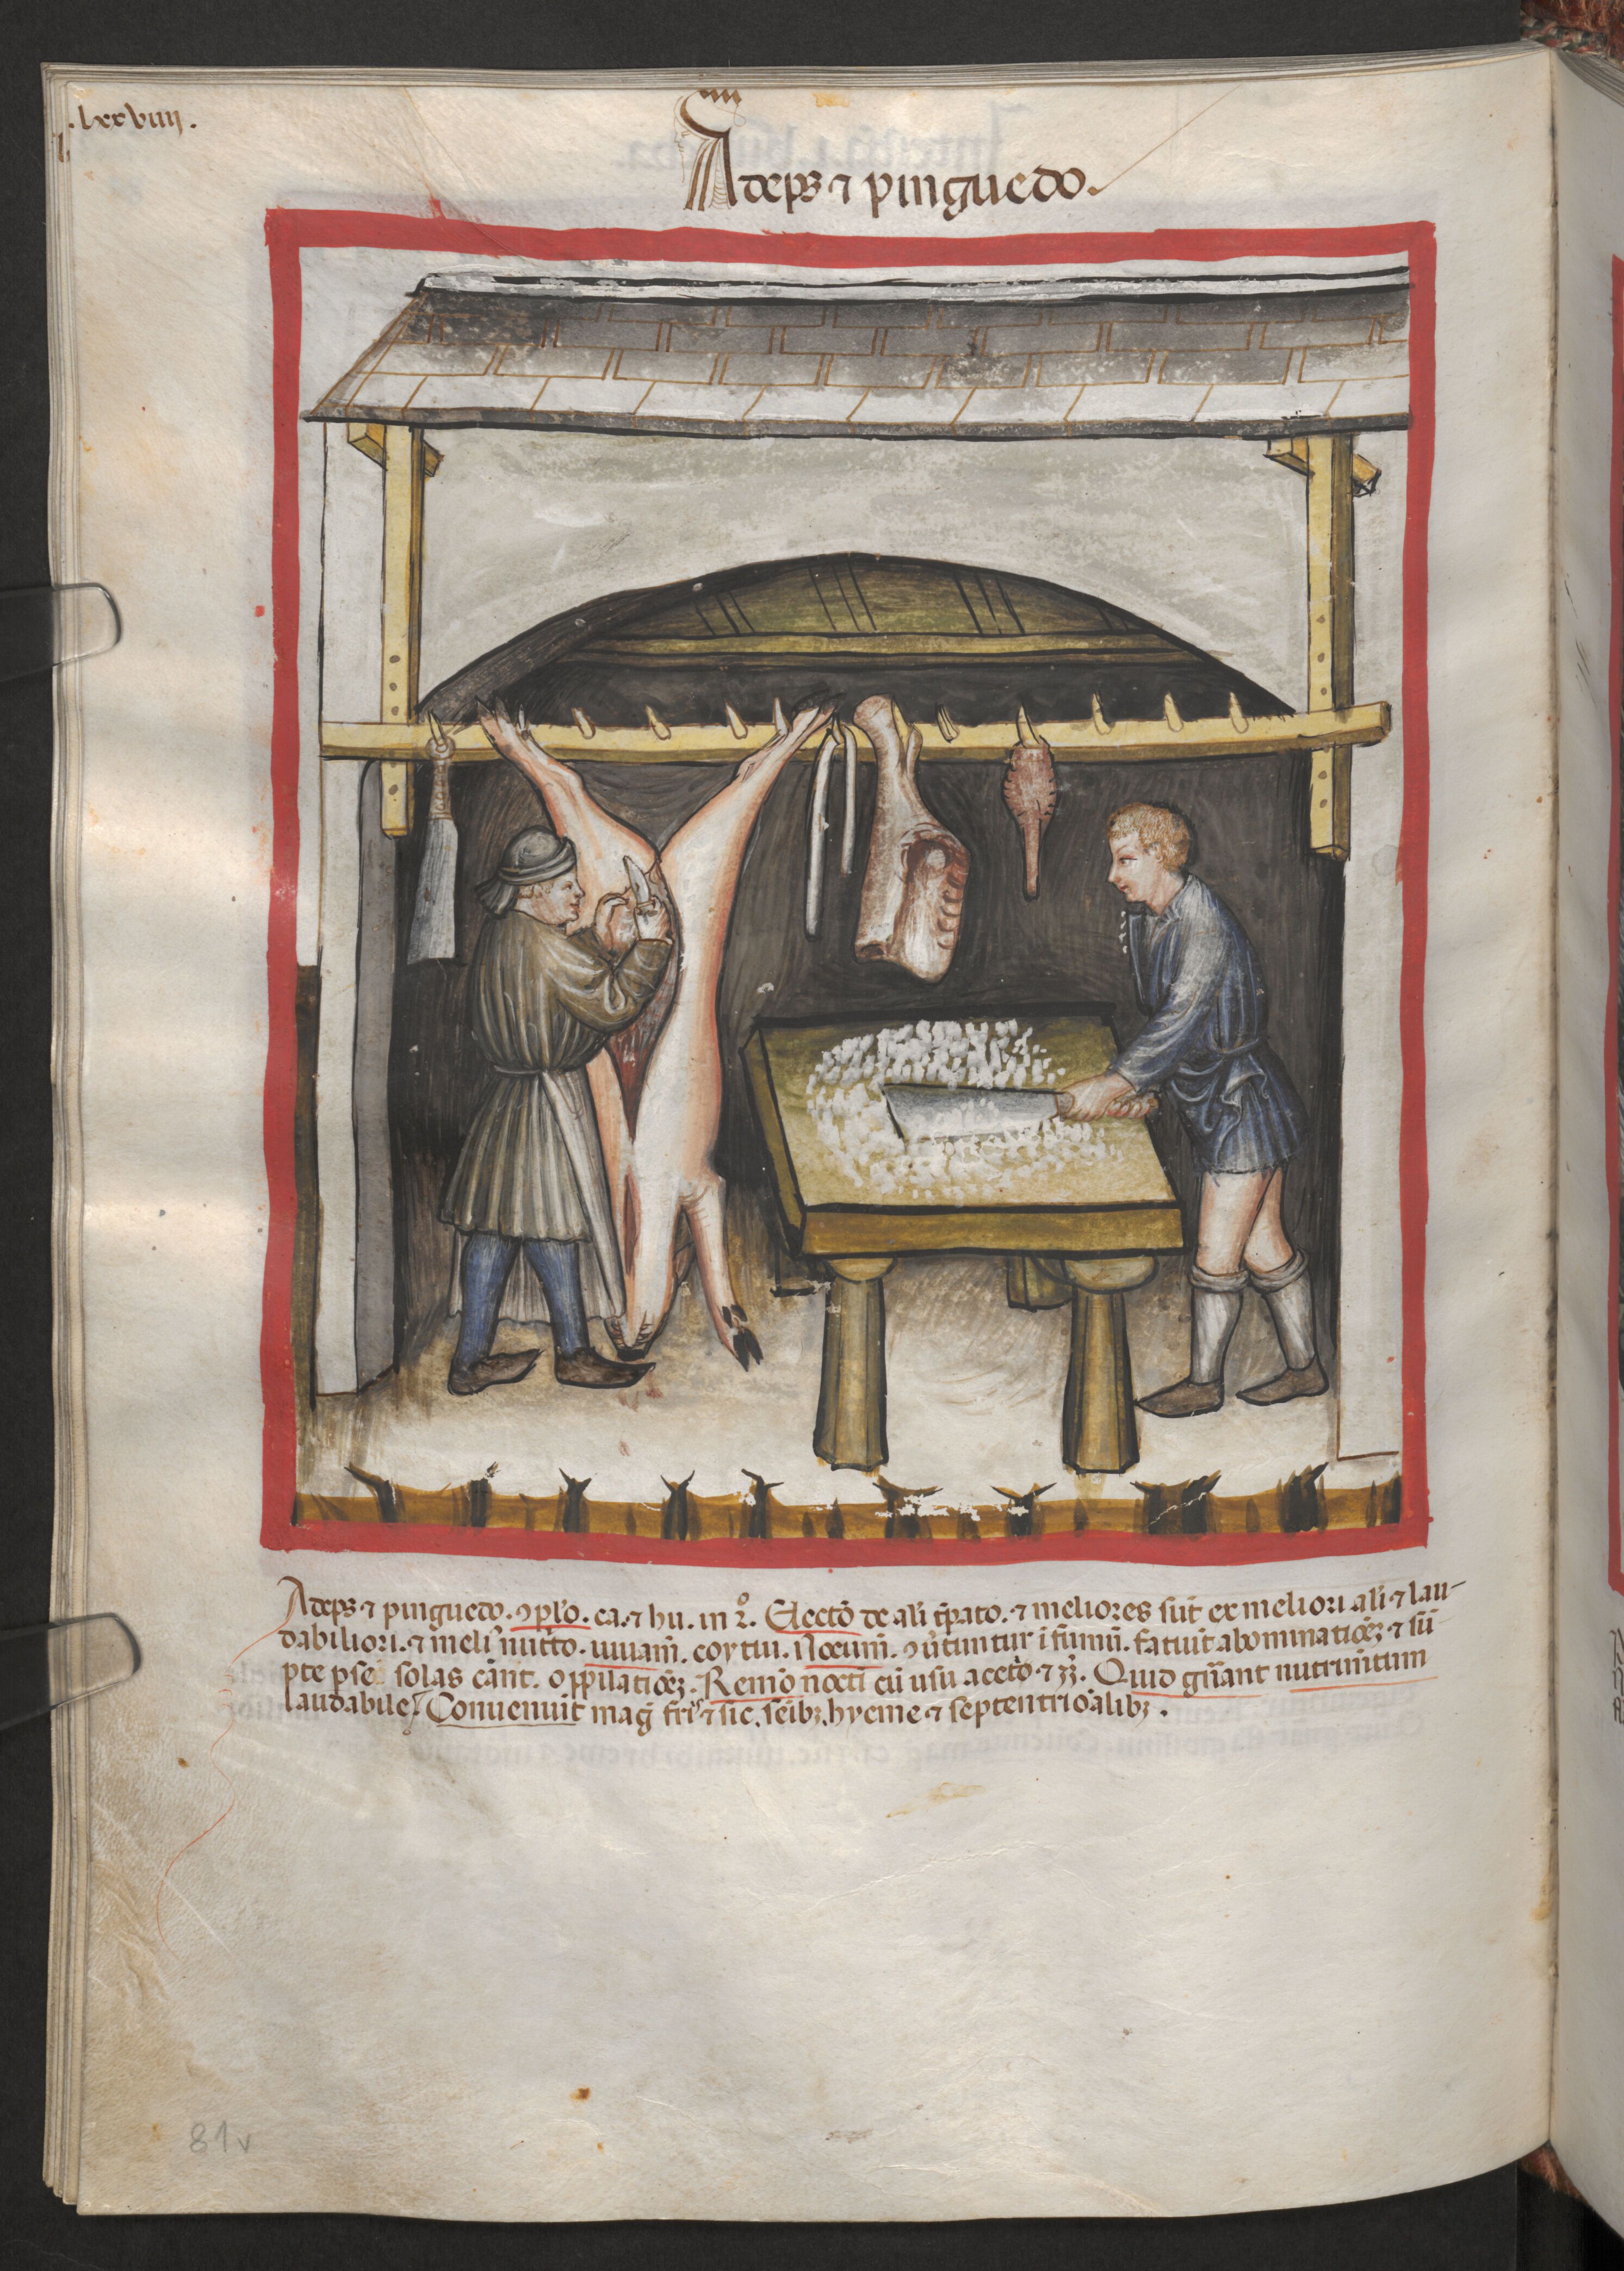
\includegraphics[width=0.9\textwidth]{Figures/Tacuinum_Sanitatis_p82L.png}
 	\caption{Example of Someone chopping meat (for sausage?) German Source and illuminations of translated work.\citep{TacSan}}
 	\label{plot}
 \end{figure}
 
 There is also discussion of beating or pounding the meat to get finer textures when desired. There were a variety of tools used for this. They used hammers/mallets, mortar and pestles, and the sides of large knives(cleavers). 
 
 This example is only for reference to the techniques used and can be used for any sausage recipe requiring fine texture and uniformity in their mixture.
 
 \begin{quote}
 	Take meat from a hot thigh [i.e. freshly slaughtered]. Remove the sinews (abߧb), blood vessels (buråq), and bones. Chop meat into fine pieces and pound it with two mallets (mi'r§b).6 Wash the stone mortar (Èajar) with salt and water and wipe it dry. Put the meat in it along with some coarse salt and pound it into paste. \cite{al2007annals}
 \end{quote}
 
 Another example text from Venice describes the making of mortadella which requires a significant amount of beating/pounding.
 
 \begin{quote}
 	[102v] To make mortadella of meat.
 	First you must take the intestines or bondole [bungs] of pork, and wash them well in many changes of water without taking out the fat that remains in them.  To disentangle/ pinch/ straighten them with salt, flour and wine, rub them with your hands, and beat/shake them very well, and then wash them in many washes of wine, and then wring the wine out of them, and place them in a pot with one pound of salt, and mix them with said salt, and then leave these things alone for four days.  Then take the meat well cleaned of the sinews that are inside it, and accompany the lean meat with fat so that it may be according to the good judgment of the one who wants to make it, and pound all the aforementioned together very thoroughly.  And for every twenty-five pounds of meat throw in two or three times ten ounces of salt, and one ounce of cracked pepper, and four pig’s hearts, six milze*, four sweetbreads, and one pennola** of liver, all from pigs, and I say this for the weight of the dish that you will have with these four types of meat together, each which will give its own liquid.  And punch a hole in the lean meat and fat with your fist, and throw said mixture*** inside, and then mix everything together again for the space of an hour spumegiando, and then add a glass of pure black wine, per the weight of the first meat, several times always spugnegiado, and then let it stand thus kneaded for the space of two or three days, it doesn’t matter. 
 	
 	(Libro novo nel qual s’insegna a’ far d’ogni sorte di vivanda (aka Messisbugo) (1557) Cristoforo Messisbugo (written in Ferrara, published in Venice -- facsimile of 1557 edition by Arnaldo Forni Editore, Bologna 2008). Work in progress translation by Ariane Helou)
 \end{quote}

\FloatBarrier

\subsection{Period stuffing methods and tools} 

The period method of stuffing could involve using a funnel. The funnel can be made of metal(Quote \ref{MetalStuffer}), horn, or ceramic.

This reference is purely for reference that they used funnels to stuff sausages in period even though it is from Arabic regions and cultures and there is no reason or evidence to the contrary for their use in Western Europe as well. In fact there is a decent amount of evidence for influence coming into Western Europe from Arabic regions with respect to cooking and sausage.

\begin{quote}
	A copper stuffer (miÈaê9ê9a) for large and small sausages. (12r) \linebreak
	 \citep[p. 87]{al2007annals}
	\label{MetalStuffer}
\end{quote}

The most complete set of instructions I have found for the actual process of stuffing sausages comes from a German source which still doesn't describe how to do the actual stuffing part but does describe what it should loop like as well as the process.

\begin{quote}
	Take the meat/ and stuff it in the intestines/ and press it firmly/ and when you see that the intestine develops bubbles/ and the meat does not come over each other??/ then tamp the intestine with a needle point or a bodkin/ then it it goes even sooner over each other/ and becomes firm/ Tie the sausage closed/.

	(Max Rumpolt’s Ein new Kuchbuch (1581)
	Palmer, Sharon trans.  Max Rumpolt’s Ein new Kuchbuch.  Self-published, 2012.)
\end{quote}



\subsection{Materials}

In period they would have used the cleaned and scraped intestines of various animals including sheep, pig, cow, rabbit, etc. Natural hog casings are fairly easy to get and should match the period version fairly well. There might be some more inconsistency in thickness do the the manual scraping process of the intestines for the period casings.

The meat used in period varied a lot. They used pig a decent amount across Western Europe but sheep, deer, cow, seafood, etc. were also used. There were some differences to our pigs now than the pigs that they had in period. The main differences between the pigs in period and those today were that the period pigs had longer legs. The other big difference is that they took longer to reach maturity with them taking around two years.

The spices were another category of materials which might have changed throughout the time period and by region. This was because different spices were more readily available in different regions and times. The only spices which were used were those specifically mentioned in either the direct recipe that was referenced, or those found in similar recipes around the same region and time period of the original recipe. The main spices used were black pepper (I used a mixture of long pepper, cubeb pepper, and standard black pepper), fennel, garlic,

Salt was an interesting material as there were different grades of it. I am using a good sea salt for my recipes as of the salts we have today the rock salts like Himalayan salt and similar were more expensive and there are direct references to sea salt in some of the texts specifically the version called "white salt" which was the re-refined version of sea salt to remove impurities. (Cuoco Napoletano: (late 15th century) Scully, Terence.  The Neapolitan Recipe Collection: (New York, Pierpont Morgan Library, MS B{\"u}hler, 19) : a Critical Edition and English Translation.  Ann Arbor, MI: University of Michigan, 2000.  Print.  ISBN 0-472-10972-3. )

\appendix

% Enter appendix text:
\section{Process}\label{a:appendix1}

\subsection{Fresh Sausage Recipe Used}

The recipe that I used for the fresh sausage was a combination of two different recipes. These recipes were from a 15th century Italian manuscript and from a 16th century German manuscript.

\begin{quote}
	When you wish to make good sausage with pork or other meat
	Take some lean meat and some fatty meat trimmed of all its sinew and finely chop.  If you have ten librae of meat, add one libra of salt, two ounces of well-washed fennel seeds, and two ounces of coarsely ground pepper.  Mix well and let set for one day.  Then take some well-washed and trimmed intestines and fill with the meat and then smoke to dry. \citep{martino2005art}
\end{quote}

\begin{quote}
	You can also well make sausages with garlic/ Take no more than fresh Speck and garlic/ cut it into the roast/ pepper it/ and see/ that you do not over salt it.  Take pig intestines/ or from a fallow deer/ clean the slime out/ and make it clean/ stuff the meat in/ thus you have a garlic sausage. \citep{rumpolt1980new}
\end{quote}

In the end I used the following actual measurements as a ratio:

\begin{itemize}
	\item 1000g Pork Shoulder
	\item 75g Garlic
	\item 30g Salt
	\item 12.5g Black Pepper
	\item 10g Fennel
	\item 200g Water
\end{itemize}


This recipe was decided on since it was a relatively simple recipe. I had also made the base recipes themselves before but in terms of flavor they were not very complex.

I also cold smoked the sausage(Figure \ref{SmokingSausage}) in my smoker(Figure \ref{Smoker}). I chose to cold smoke the sausage because of the wording of "smoke to dry" which seems to indicate a slower lower temperature smoking process. The is in comparison to smoking in the chimney or over the fire which is more of a hat smoking/roasting process.

 \begin{figure}[!htb]
	\centering
	\includegraphics[width=0.45\textwidth]{Figures/Messenger_creation_8ca9e75e-8d85-4b6f-bd27-b4976f07179f.png}
	\caption{The outside of my Smokehouse}
	\label{Smoker}
\end{figure}
\begin{figure}[!htb]
	\centering
	\includegraphics[width=0.45\textwidth]{Figures/2024-04-26-11-13-05-315.jpg}
	\caption{Sausages Smoking}
	\label{SmokingSausage}
\end{figure}

\FloatBarrier

\subsection{Cured Sausage Recipe Used}

The recipe that I ended up using was based on a few different examples given in various manuscripts for a dried sausage used in salads. Most of the examples were at the end of the time period i was looking at and were found in a couple different German manuscripts. This example of cured/dried sausage was from a 16th century German manuscript.

\begin{quote}
	 “Italian sausages.  Take several pounds of meat that contains neither skin nor bones.  Also take bacon *, cut it into cubes; chop the meat, then mix the bacon cubes into it and take salt and peppercorns and also mix that in.  Contain it in gut casings and hang these sausages in the chimney so that they become dry.  Boil them with a salad.  (Dat klene Kakeboeck, \#23)  [Hamburg, 1570 -JDF]
	
	“Given the risk of failure, the loss of weight through drying, and the high quality of fresh meat required, these were an expensive pleasure.  They were eaten sliced thin, with bread, cheese, and condiments, most famously by church reform activists in public defiance of the Lenten fast in 1522.”
	
	* The German term “Speck” most likely does not refer to modern, US- or Canadian-style cured and smoked bacon.  Salted, unsmoked fatty pork meat is more likely.  Curing may well be part of the process, but we have not found specific recipes.  Some works distinguish between salted and fresh Speck, and our assumption is that fresh Speck is simply fresh fatty pork meat.
	
	(The Kitchen, Food, and Cooking in Reformation Germany (16th century)
	Bach, Volker.  The Kitchen, Food, and Cooking in Reformation Germany.  
	Lanham: Rowman \& Littlefield, 2016.  Print.  ISBN 1442251271.)
	
\end{quote}

The next example translates the term speck as bacon or salt pork. This does not seem consistent with the other recipes and so probably actually refers to uncured belly or back bacon instead. This would match the other excerpts where speck is included in sausage.

\begin{quote}
	Stuffing sausages, Italian style. 
	Take a few pounds of meat, take out the tendons, skin it, slice it into cubes, add some bacon [salt pork] and salt, black pepper, mix it together and stuff the intestines, afterwards, smoke these, roast it for salads. 
	
	(The Science of Cooking (mid-16th century) Gorsuch, Glenn ed. Kovacs, Bence trans.  Self-published, 2017.)
\end{quote}

The next recipe for salad sausages includes beef as a part of the meat. This was not uncommon and in fact some recipes include other animals like deer.

\begin{quote}
	23.  If you would make a good sausage for a salad
	Then take ten pounds of pork and five pounds of beef, always two parts pork to one part of beef.  That would be fifteen pounds.  To that one should take eight ounces of salt and two and one half ounces of pepper, which should be coarsely ground, and when the meat is chopped, put into it at first two pounds of Speck, diced.  According to how fat the pork is, one can use less or more, take the Speck from the back and not from the belly.  And the sausages should be firmly stuffed.  The sooner they are dried the better.  Hang them in the parlor or in the kitchen, but not in the smoke and not near the oven, so that the Speck does not melt.  This should be done during the crescent moon, and fill with the minced meat well and firmly, then the sausages will remain good for a long while.  Each sausage should be tied above and below and also fasten a ribbon on both ends with which they should be hung up, and every two days they should be turned, upside down, and when they are fully dried out, wrap them in a cloth and lay them in a box.
	
	(Sabina Welserin’s cookbook (1553) Armstrong, Valoise, trans.  Sabina Welserin’s cookbook.  Self-published, 2001.)
\end{quote}

The actual recipe that I used/will use for making these sausages will be the following ratios:

\begin{itemize}
	\item 1000g Pork Shoulder
	\item 150g Pork Belly (1/4in Cubed)
	\item 35g Salt (Sea Salt)
	\item 10.5g Black Pepper (Very Coarsely ground/cracked)
	\item 100g Water
\end{itemize}

I chose to use pork belly because I am unable to get fatty pork loin/back without much difficulty. I am very roughly cracking the black pepper that I am using as a nice middle ground between whole peppercorns and coarsely ground. The other ratios are based off of the last excerpt where I used the 15lbs of meat to determine the other ratios.

\subsection{Bacon Recipe}

The bacon that i decided to make was process described in a 16th century German Manuscript.

\begin{quote}
	And when bacon is to be had in the towns and country the same should be kept provisioned at all time. And if it were the case that this bacon should hang too long and there was concern that it was growing too old and spoiling, the same should be fed to and sold among the troops over time and replaced with new. That way, you will always have a good supply. But there must be good care in this regard that the bacon be hung up in such places and kept with smoke and air drying as it should be. Where it is not treated this way, it spoils, that is why these measures must be taken. The same should also be done with other meat, be it of cows, oxen, and so forth, when a garrison can have them they should be slaughtered and nicely and cleanly laid in salt and lay up in store. When such meat is kept clean, it will keep an entire year. When it is slaughtered, it must be chopped to pieces and the blood washed out and the meat allowed to cool. Then it is laid into casks with salt and salted well, and when one wishes to eat of it, it should be hung up in the smoke for a day or more and then cooked. But because it has lain in the salt, it has taken on much salt to itself and one must not use as much salt in cooking as one would with meat cooked fresh.
	
	(Besatzung (Garrison) (1563) Fronsperger, Leonhart.  Besatzung (Garrison).  Volker Bach trans.  Frankfurt am Main, 1564.)
\end{quote}

This excerpt is interesting because it includes the instruction to smoke the bacon for a short period before eating. This was actually an uncommon practice but obviously one which is considered. This might be one of the earlier mentions of bacon being smoked as around the same time period it is mentioned in France that it the most desirable bacon is that which has fat that is firm and white (not smoked). For this reason I will include both smoked and non-smoked bacon as well as dry cured.

\subsection{Process of making the sausage}

I first broke the meat up into two 2kg batches, one for each recipe, and the measured out each of their respective salt and spices. I then chopped the meat until i grew tired and stopped noticing a difference, chilled that one, and then chopped the other batch. Once each batch was chopped I moved on to the mortar and pestle for the pounding/beating and mixing in of the spices. After each mixture was made i then used the funnel to stuff them into the natural casings that I had. I then cold smoked them for a couple of hours. Finally, for safety I then vacuum sealed the fresh sausage and cooked them at 150F\textdegree in a water bath for a few hours to essentially can them. This also mimics the process of boiling them for a couple of hours as some recipes direct while ensuring the product is safe for the couple of weeks of storage required for prepared food at Pennsic.


\subsubsection{Chopping, Beating, and Mixing}

I first broke down the pork shoulder, removing the bone first then making thumb sized pieces(Figure \ref{Breakdown}). Once I had reasonably sized pieces I would then use my cleaver to chop the meat until it resembled roughly ground meat(Figure \ref{Chopping}). I could also get a general idea on the progress by the stickiness of the meat as it should get somewhat sticky as it gets processed and the cell walls start to break down. 

Once I wasn't making much progress with the knife(and I was getting a sore wrist) I moved on to the large Mortar and Pestle(Figure \ref{MortarPestle}). The mortar and pestle was similar in size and shape to the on found in Figure \ref{MortarIlumination}. I added the various dry ingredients(along with the garlic) and mixed/pounded the sausage mix for a bit. I then added in the required water in a couple of batches and beat until incorporated and back to sticky and not watery/wet. once all of the water was beat in I then beat/pounded it until it had the tackiness that I recognized and could stick to my hand upside down (Figure \ref{sticking}).

 \begin{figure}[!htb]
	\centering
	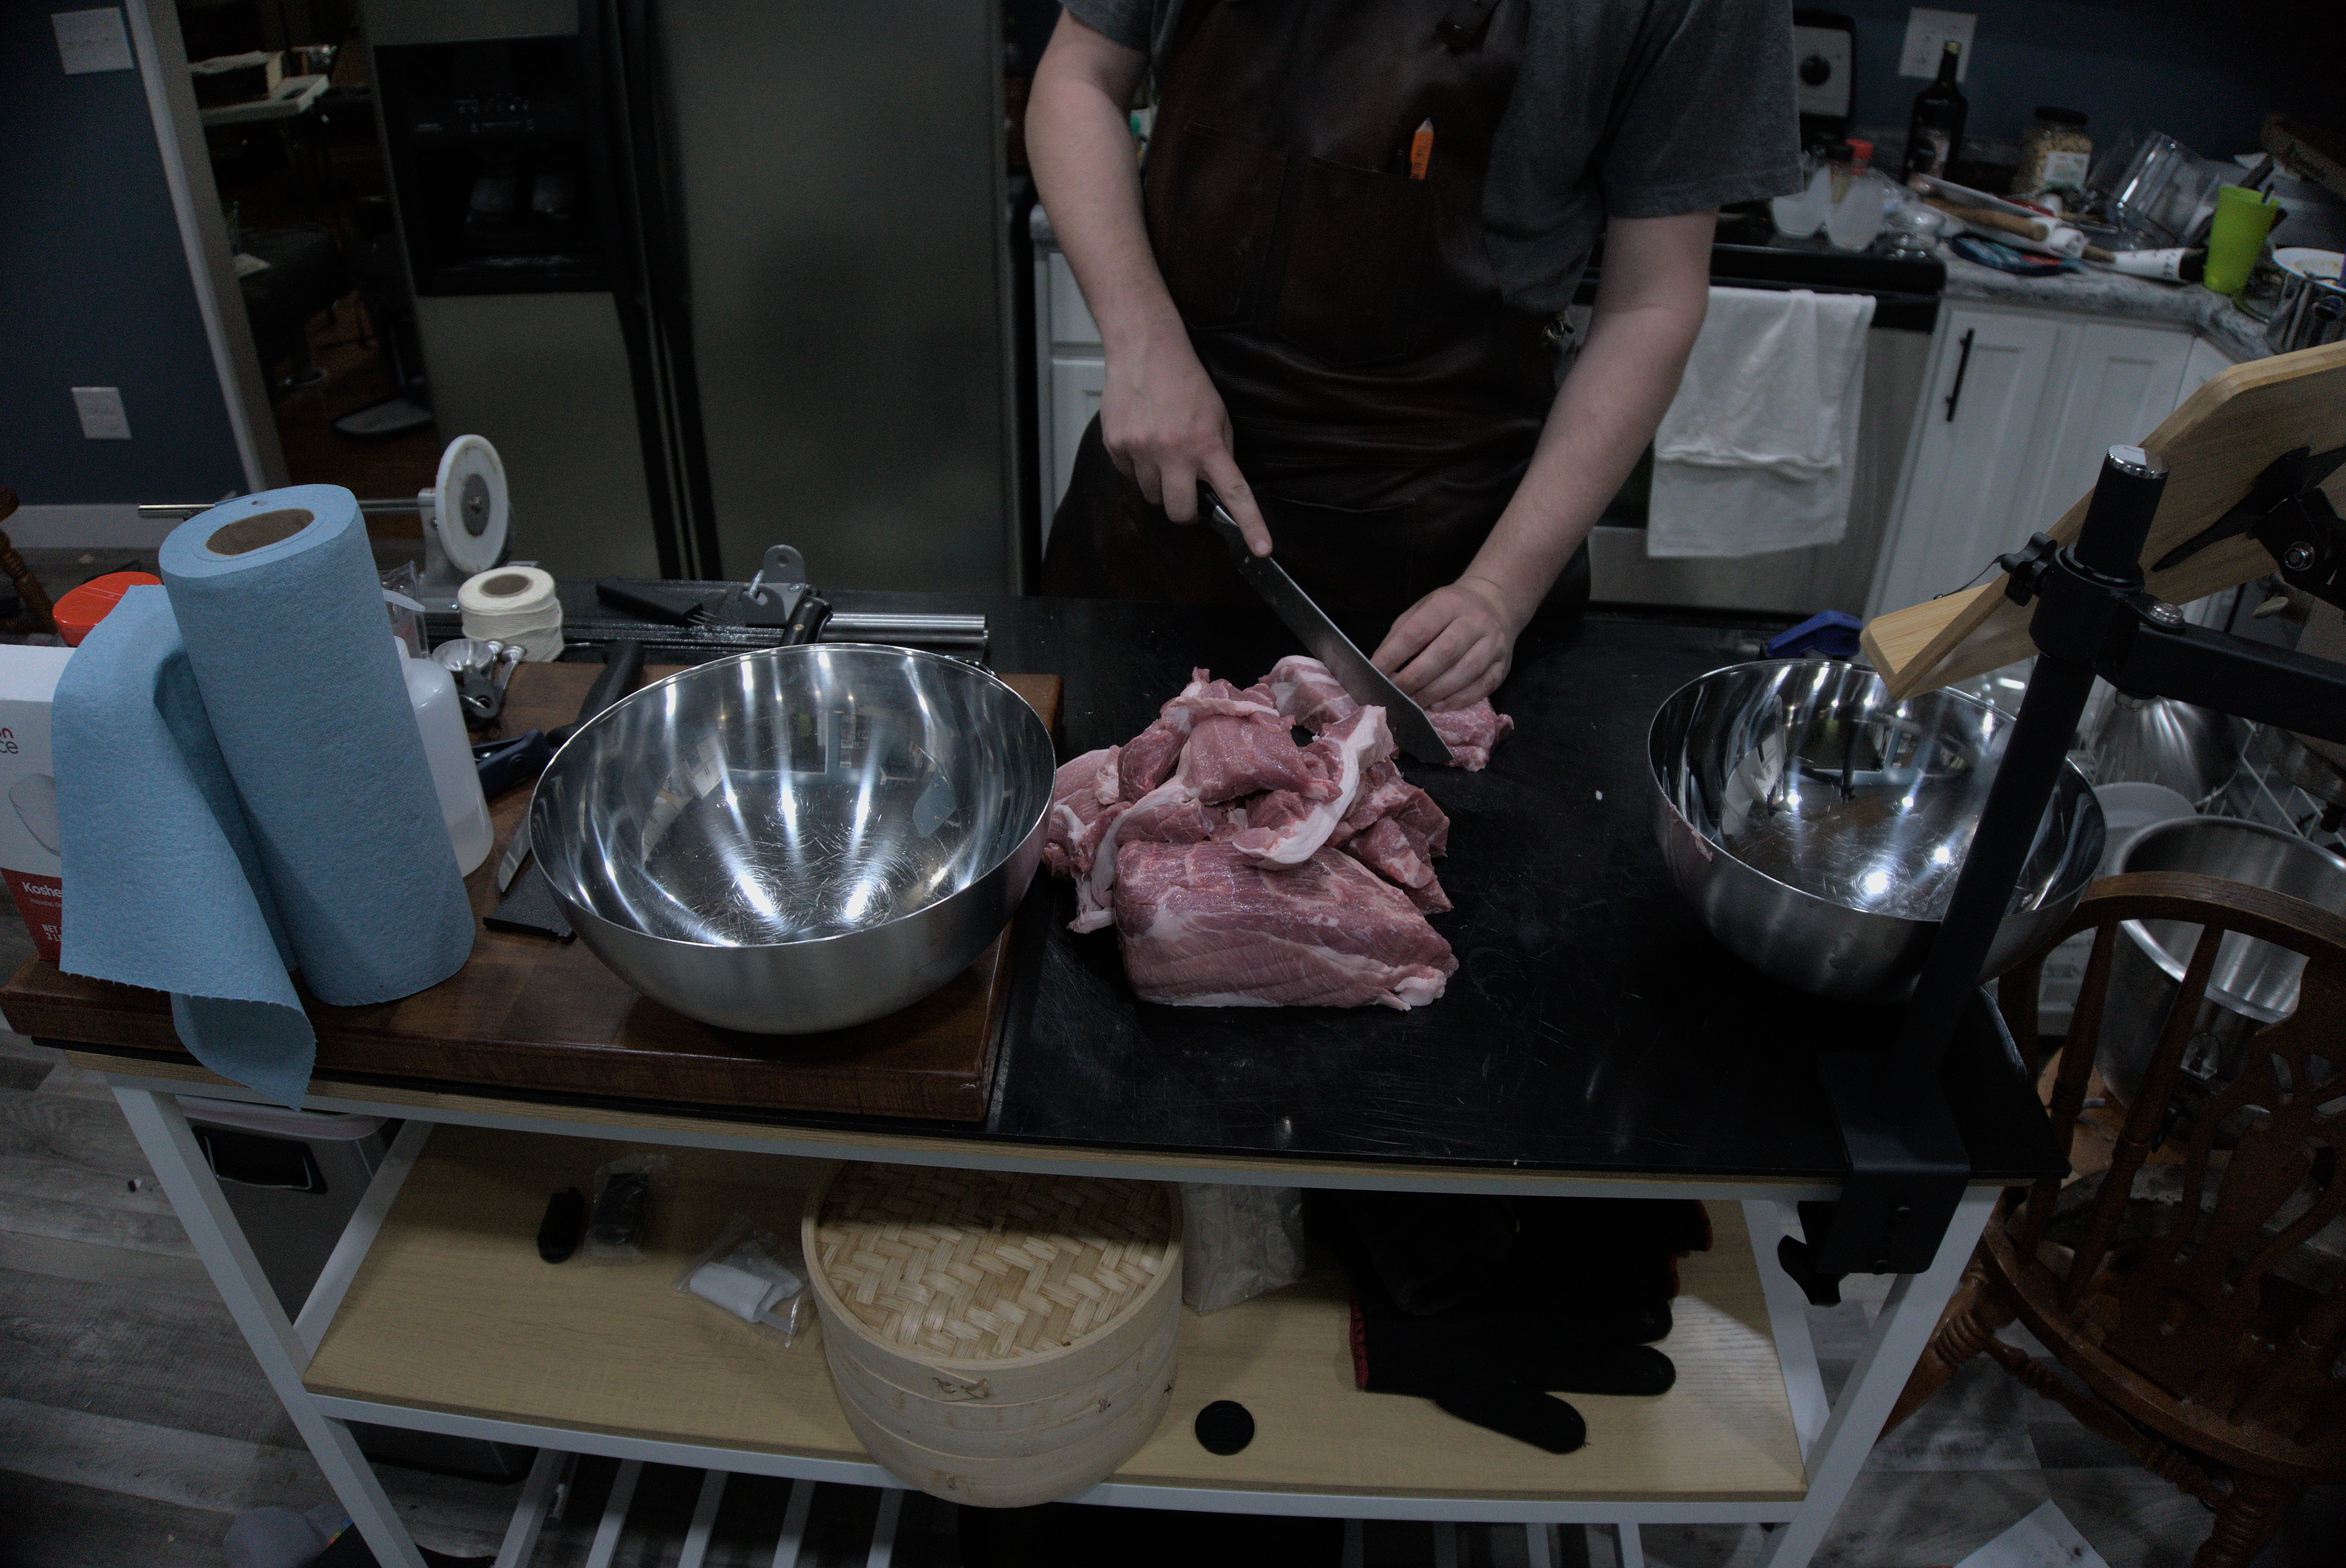
\includegraphics[width=0.9\textwidth]{Figures/20240524_0088.jpg}
	\caption{Breaking down the pork shoulder}
	\label{Breakdown}
\end{figure}
 \begin{figure}[!htb]
	\centering
	\includegraphics[width=0.9\textwidth]{Figures/20240524\_0097.jpg}
	\caption{Chopping the meat with a cleaver}
	\label{Chopping}
\end{figure}
 \begin{figure}[!htb]
	\centering
	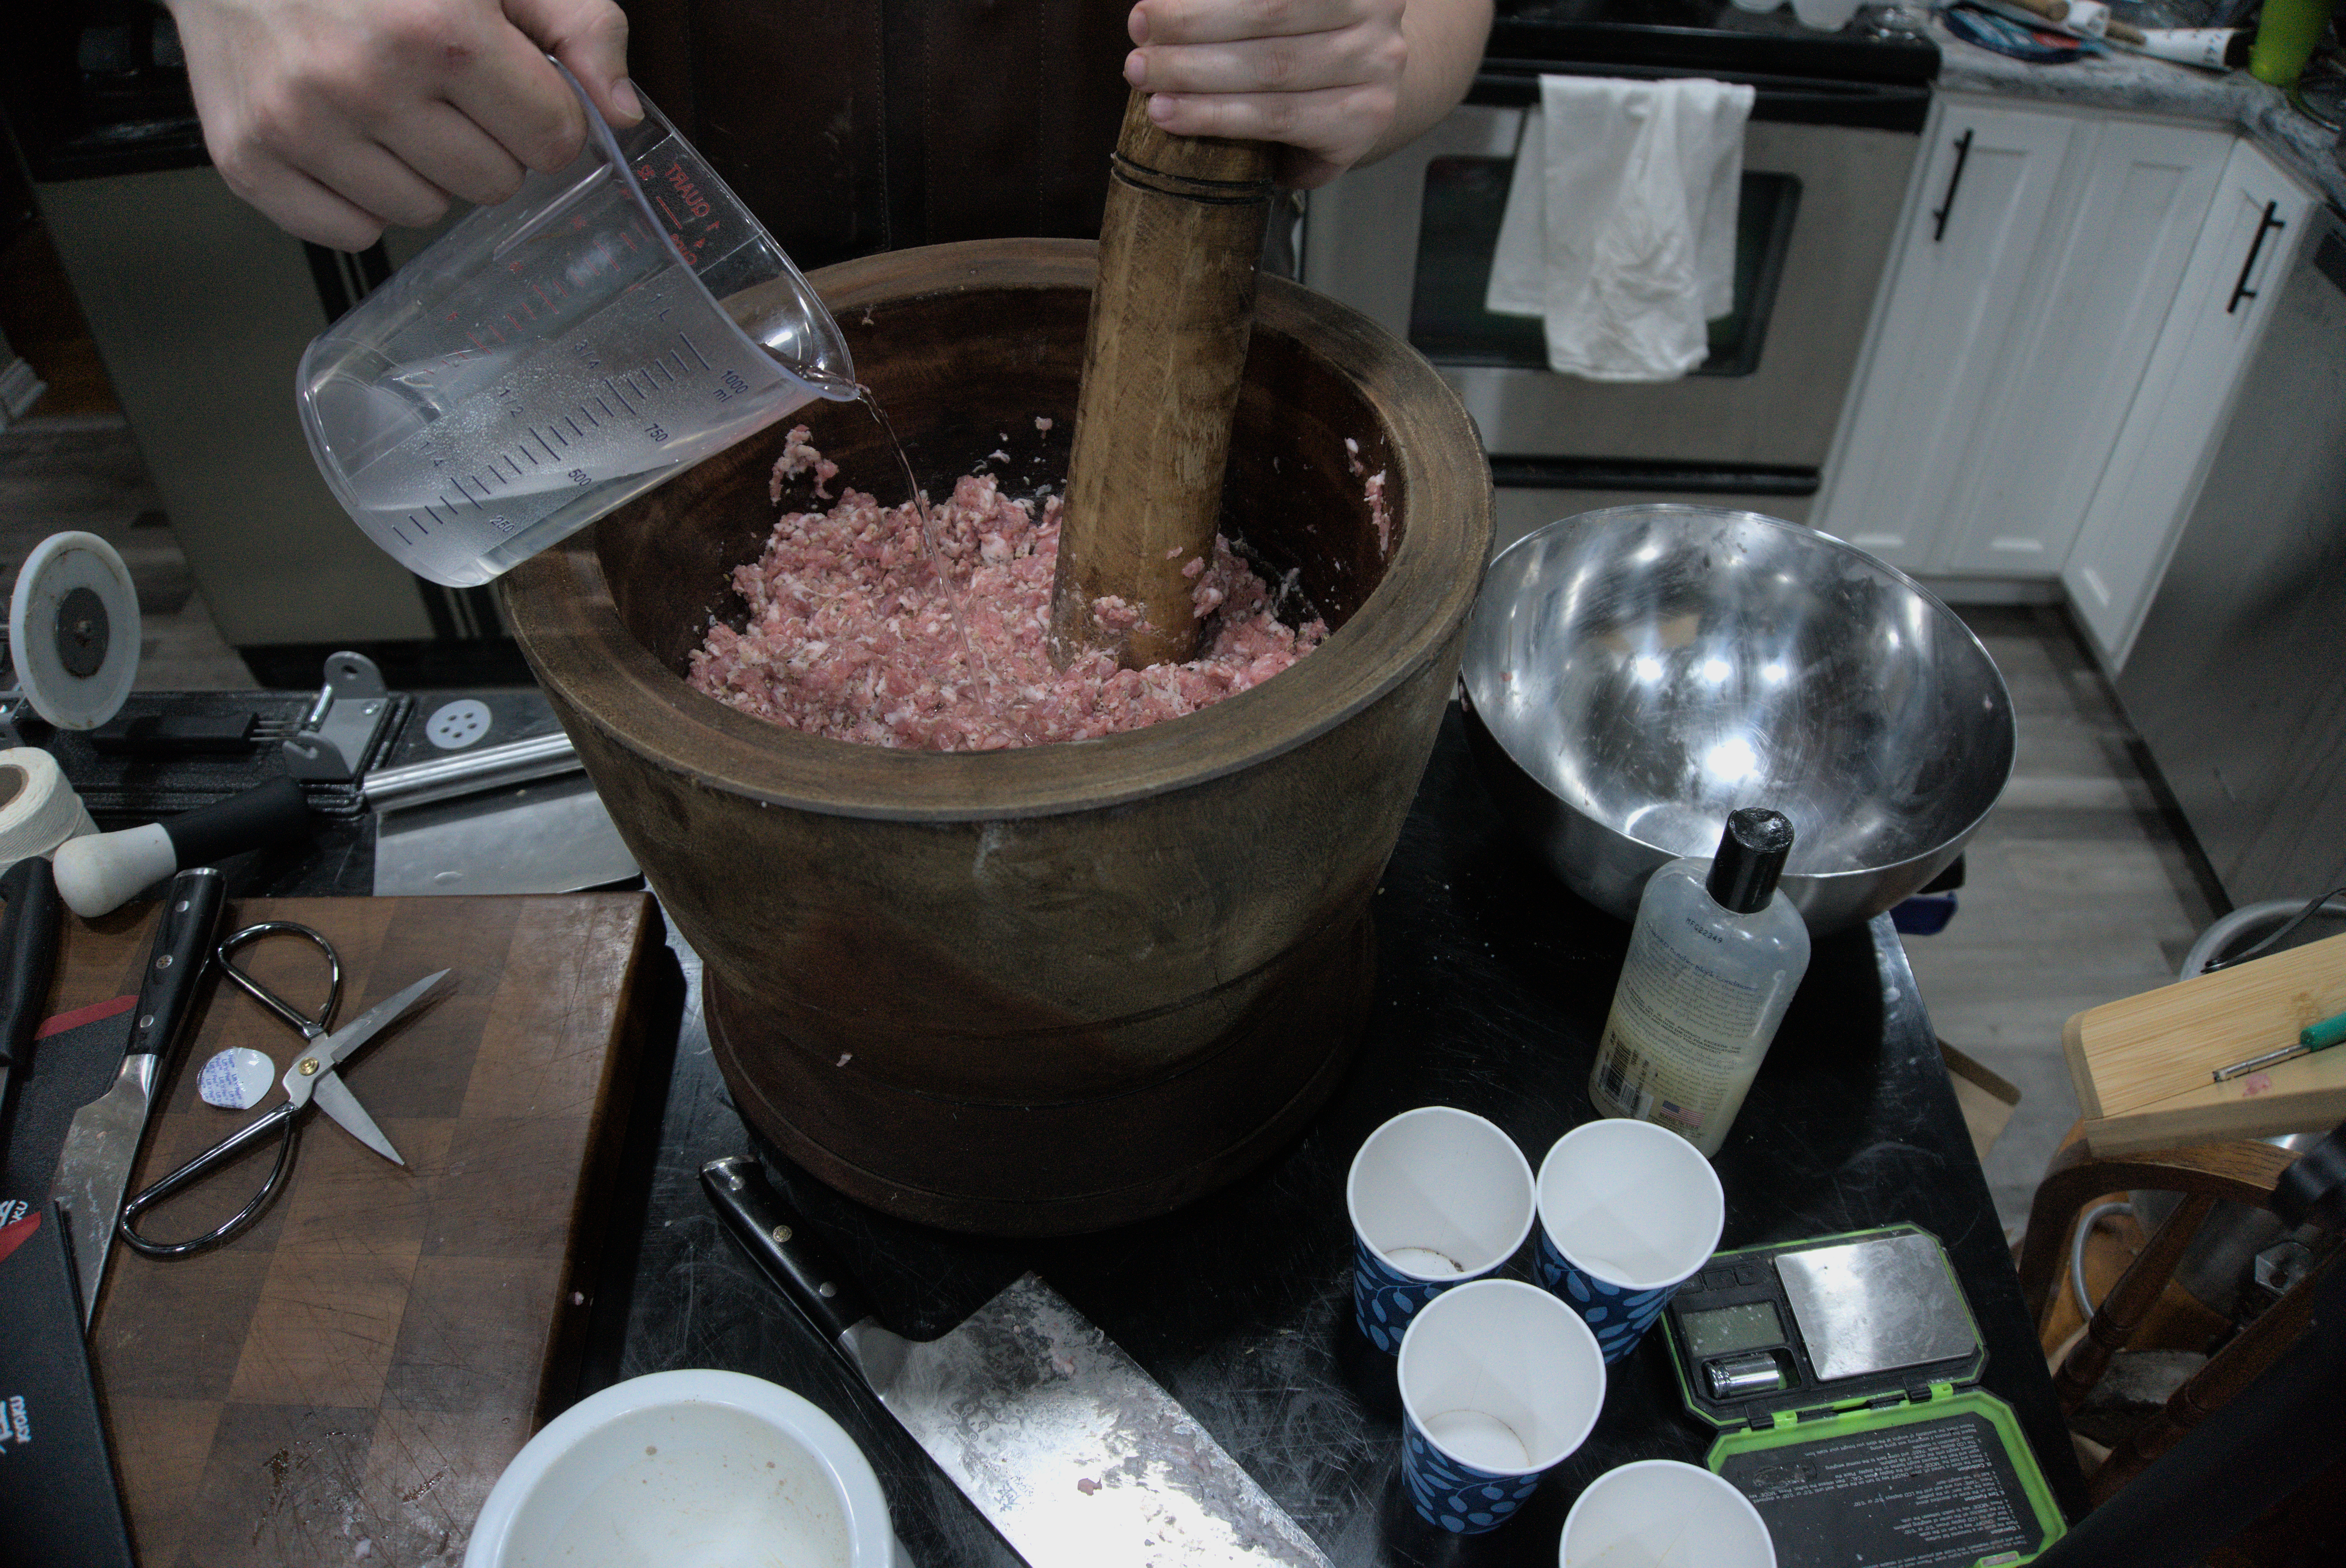
\includegraphics[width=0.9\textwidth]{Figures/20240524_0108.jpg}
	\caption{Pounding the meat with a large Mortar and Pestle}
	\label{MortarPestle}
\end{figure}
\begin{figure}[!htb]
\centering
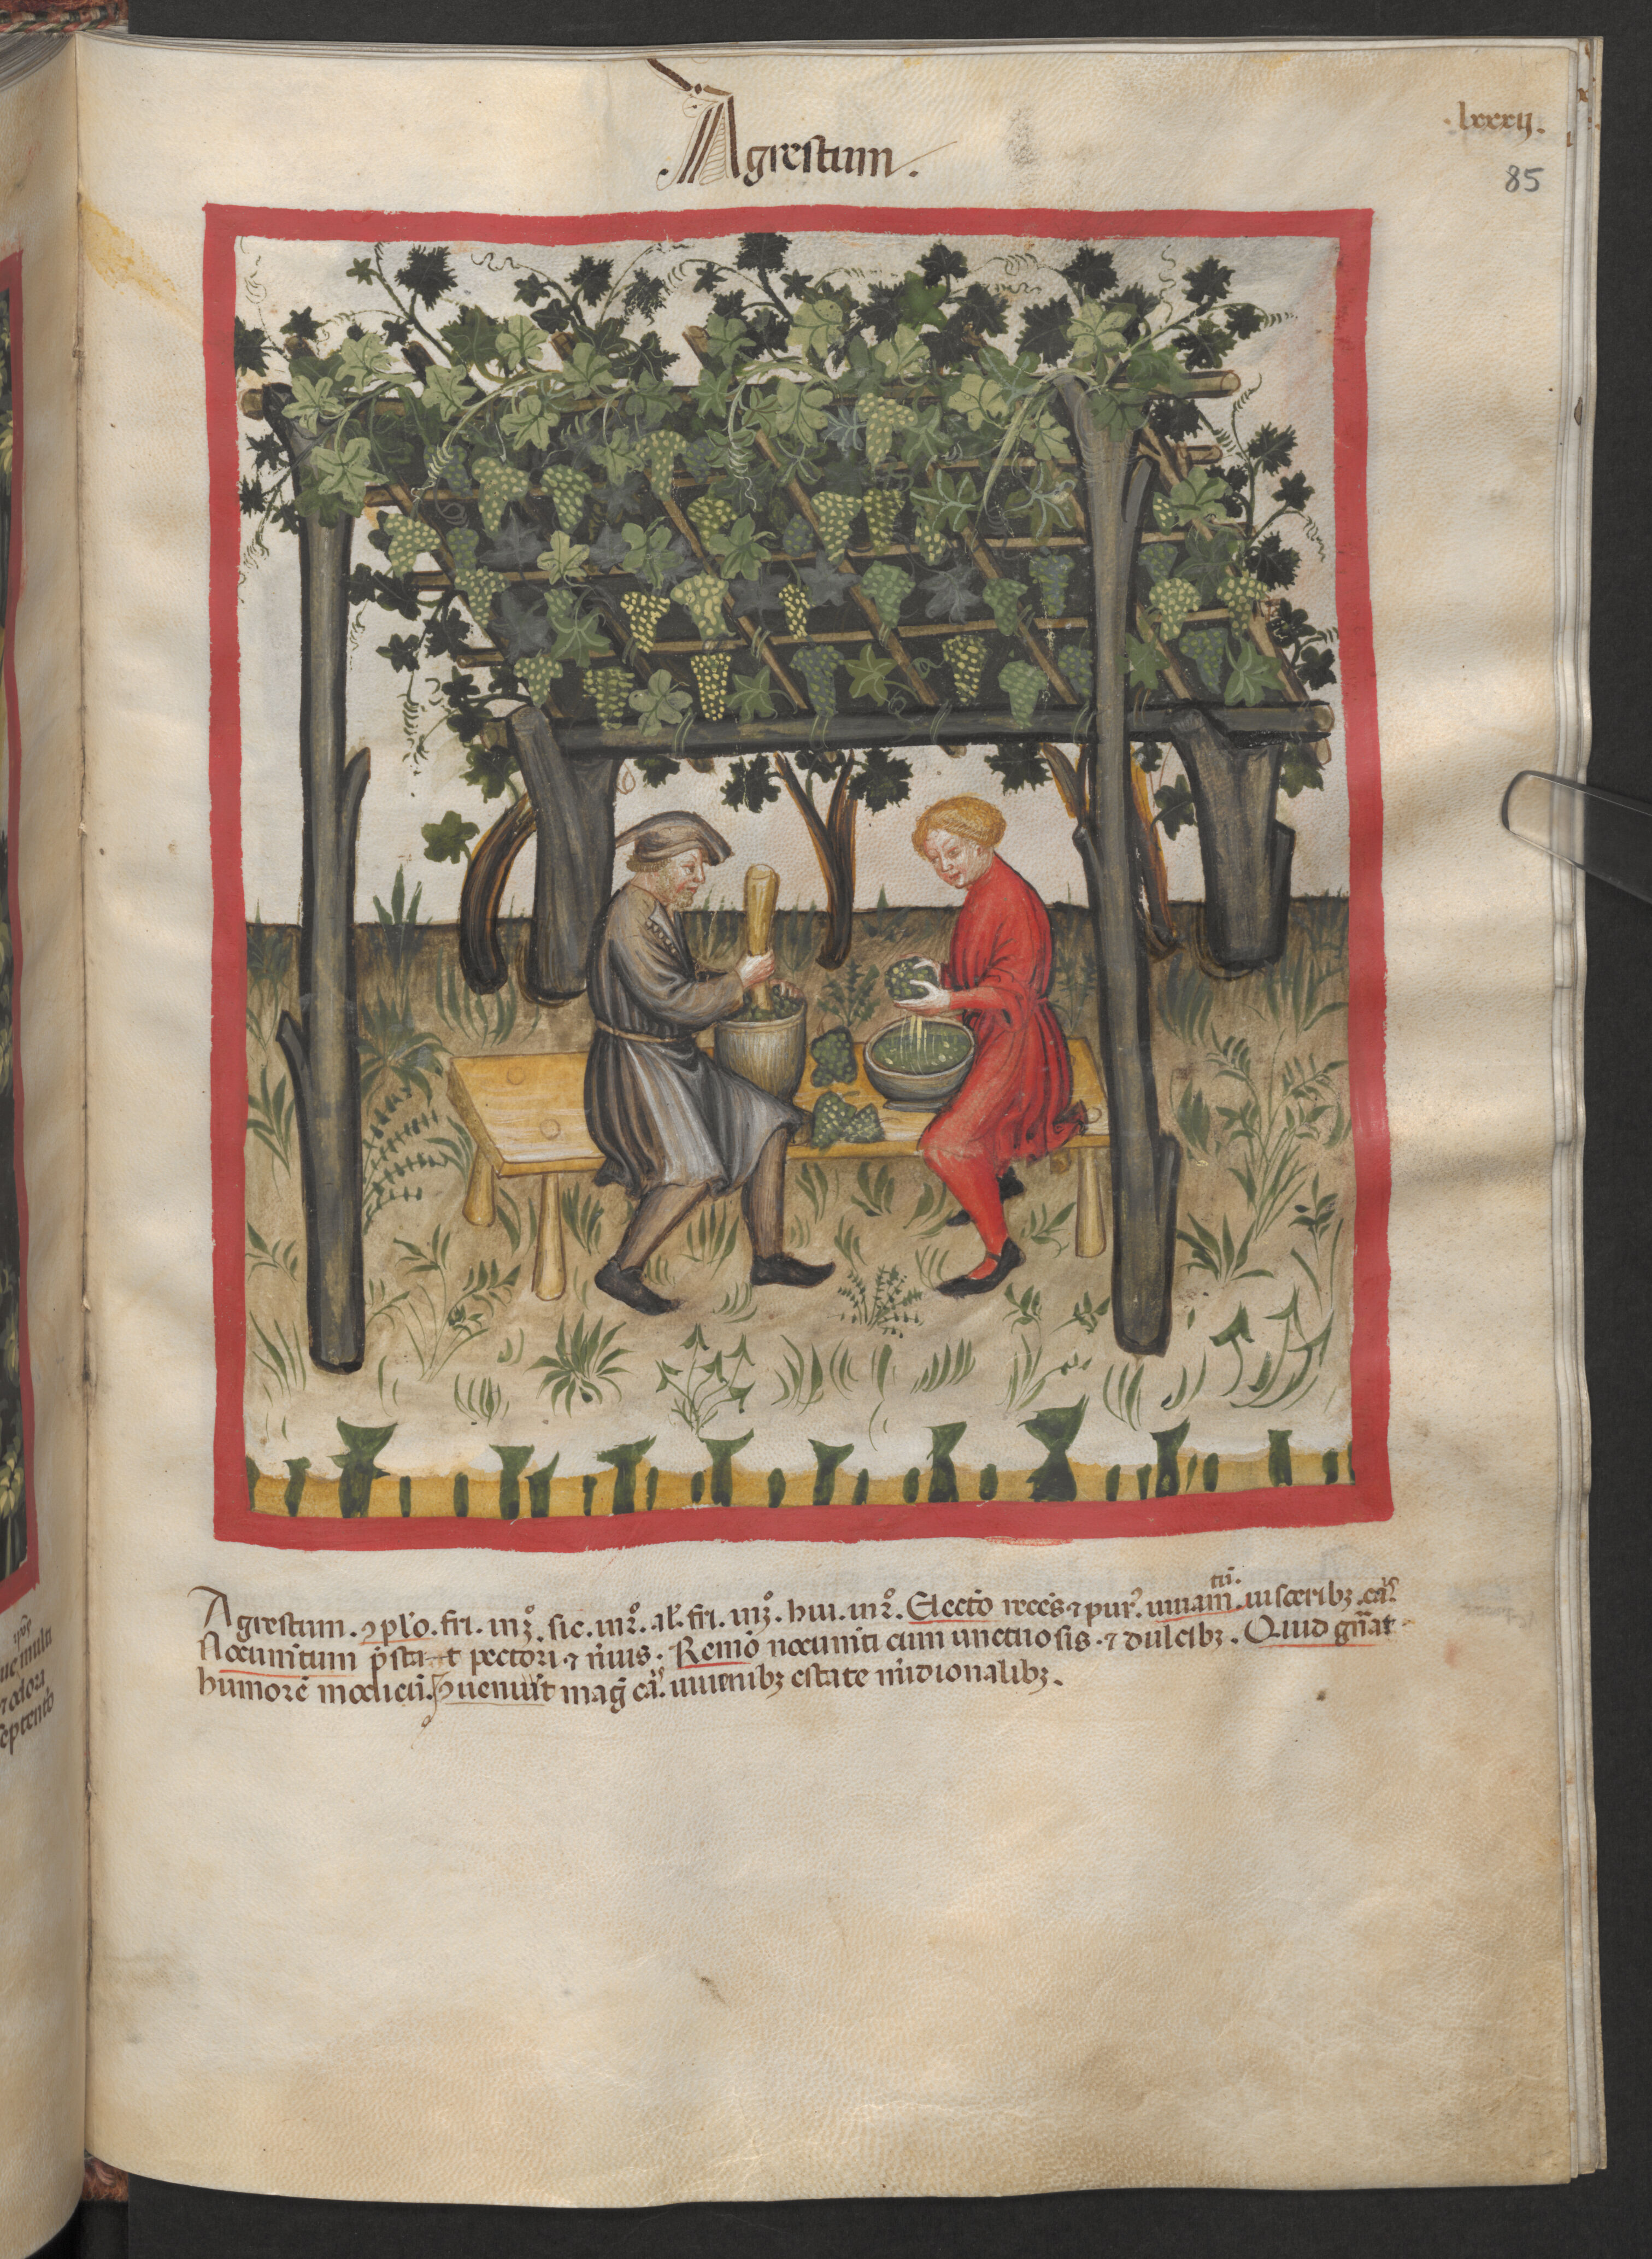
\includegraphics[width=0.9\textwidth]{Figures/Tacuinum_Sanitatis_p85R.png}
\caption{Example of a mortar and pestle used in period \citep{TacSan}}
\label{MortarIlumination}
\end{figure}
 \begin{figure}[!htb]
	\centering
	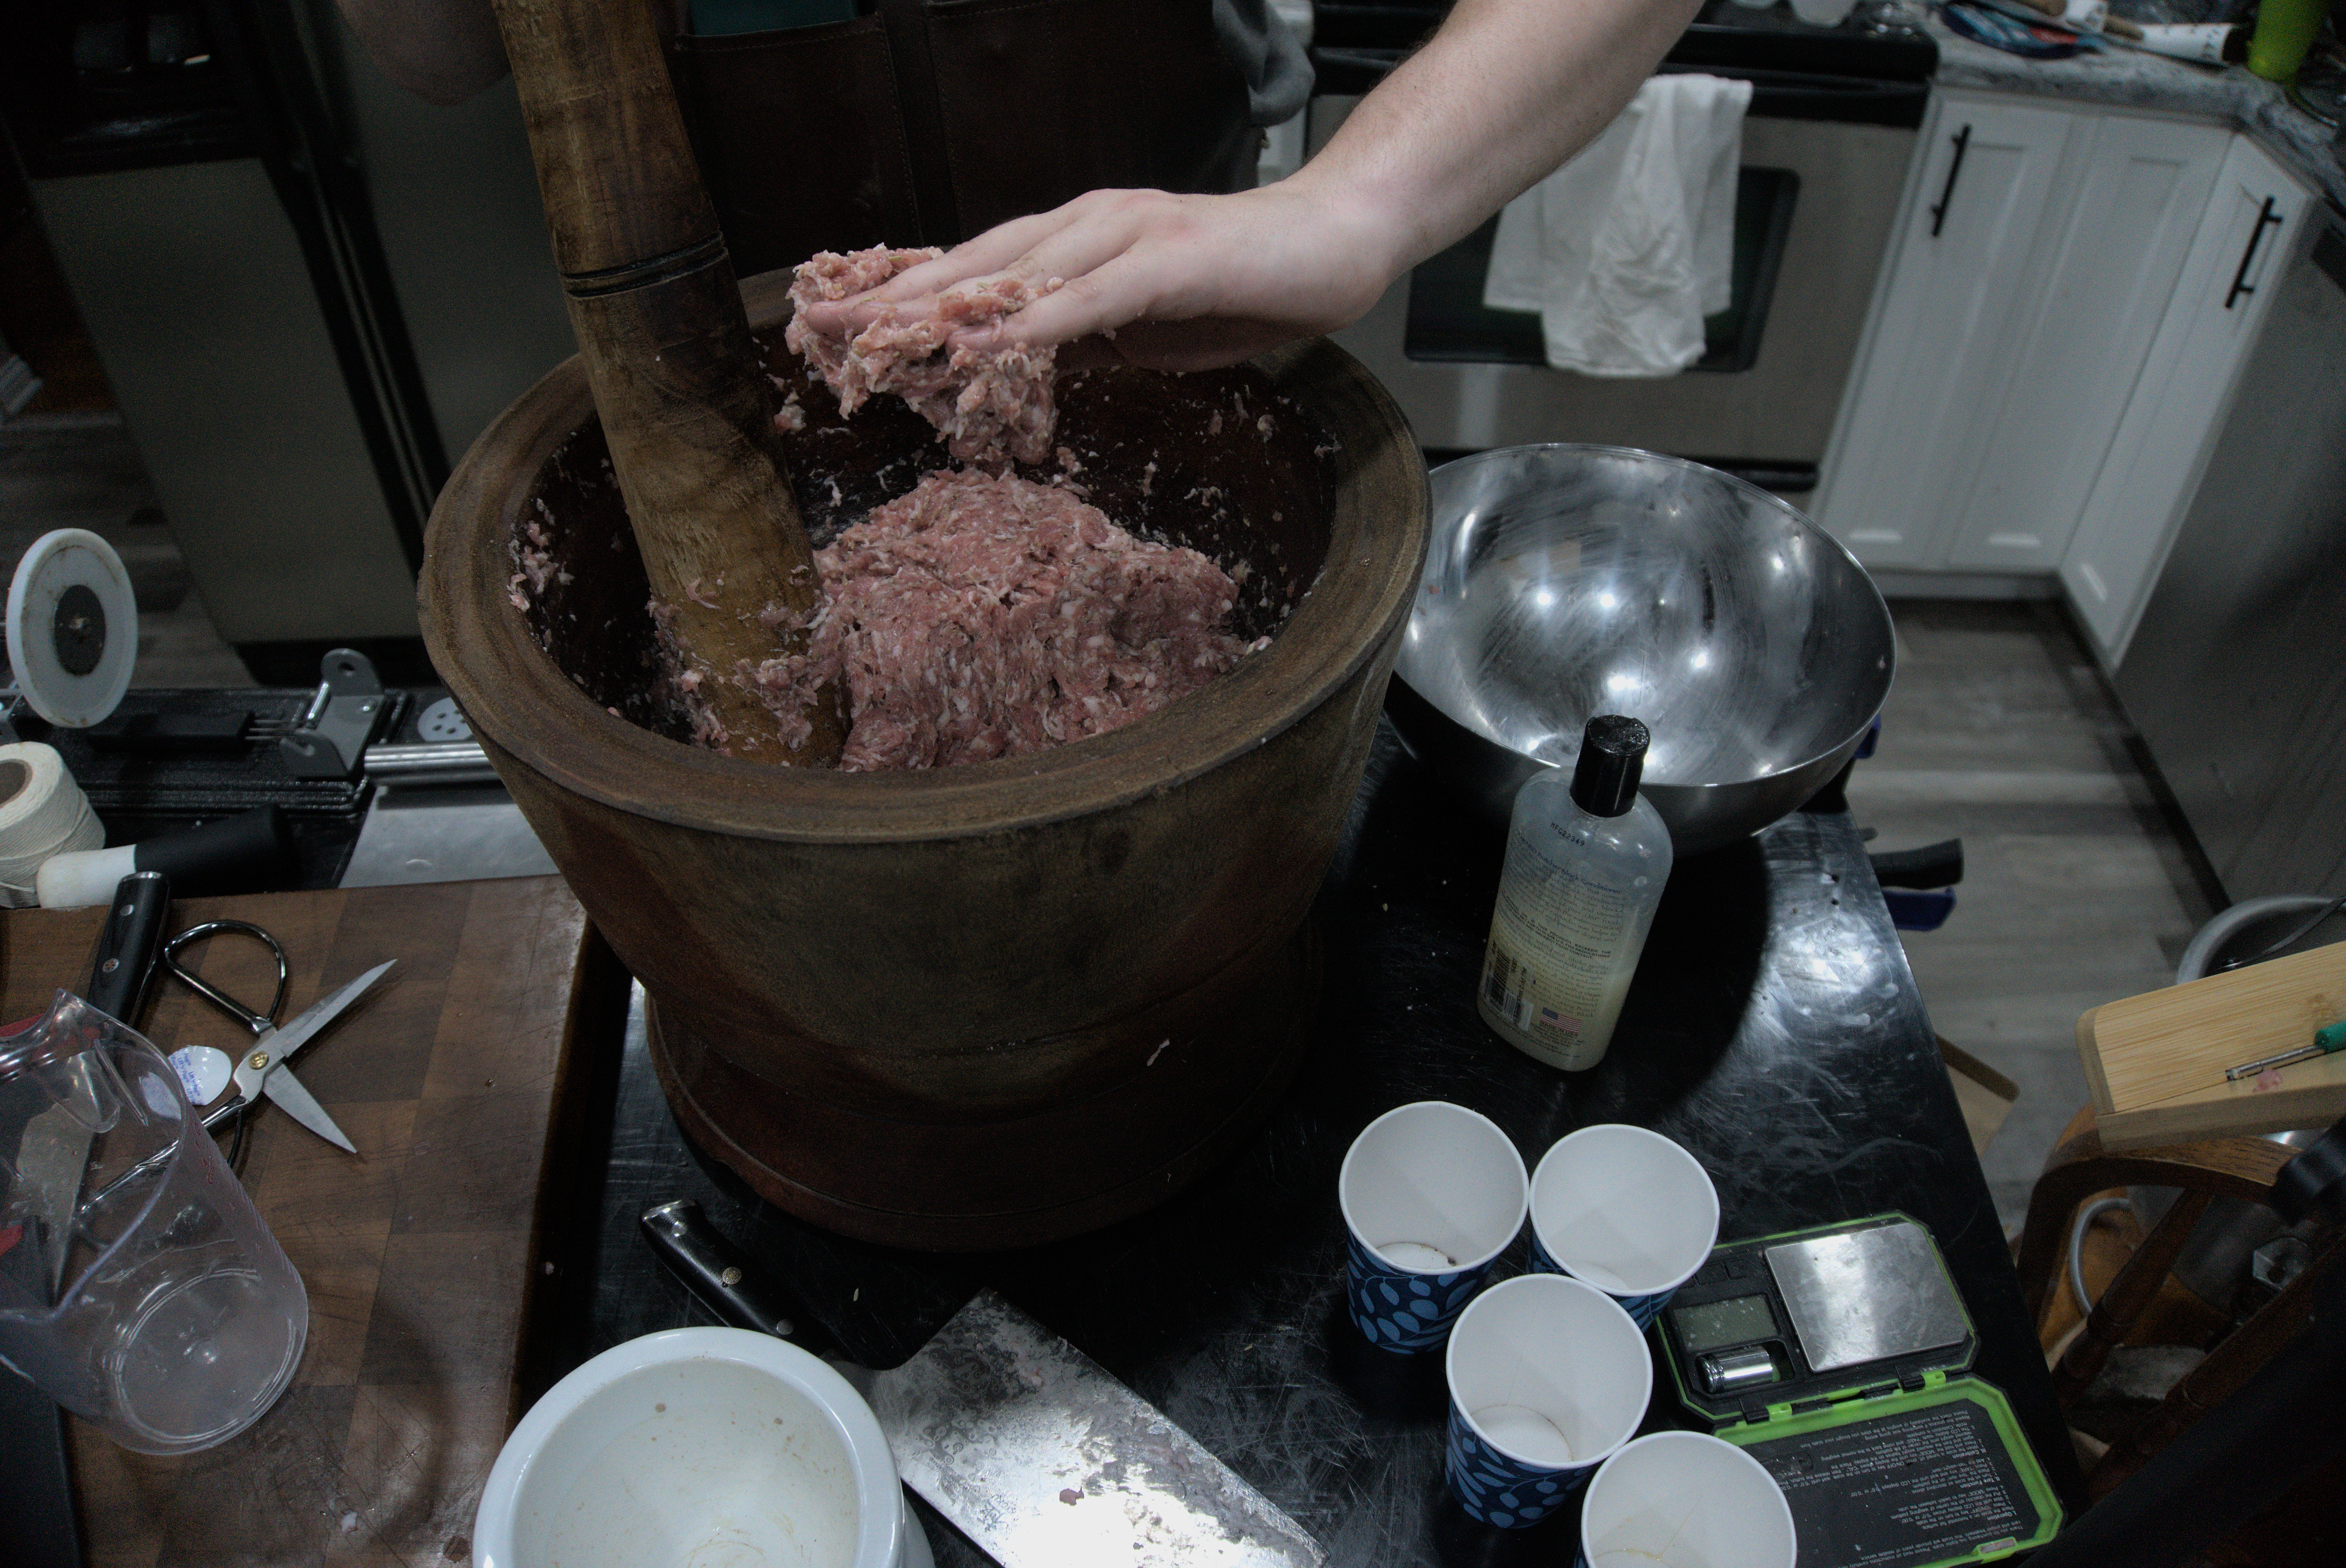
\includegraphics[width=0.9\textwidth]{Figures/20240524_0113.jpg}
	\caption{Meat Sticking to upside down hand}
	\label{sticking}
\end{figure}

\FloatBarrier

\subsubsection{Stuffing Funnels}

For stuffing the sausage I used a funnel (Figure \ref{stuffer}) to match a possible period method. The size of the neck of the funnel is a fairly important size to get right. If it is too small it is very difficult to actually stuff the sausage while a larger neck allows for easier stuffing it needs to be able to have the casings fed onto the outside of the neck. It worked but was definitely not a speedy or very easy method. The funnel  took about [Replace with actual time when made] to stuff the sausages.

\begin{figure}[!htb]
	\centering
	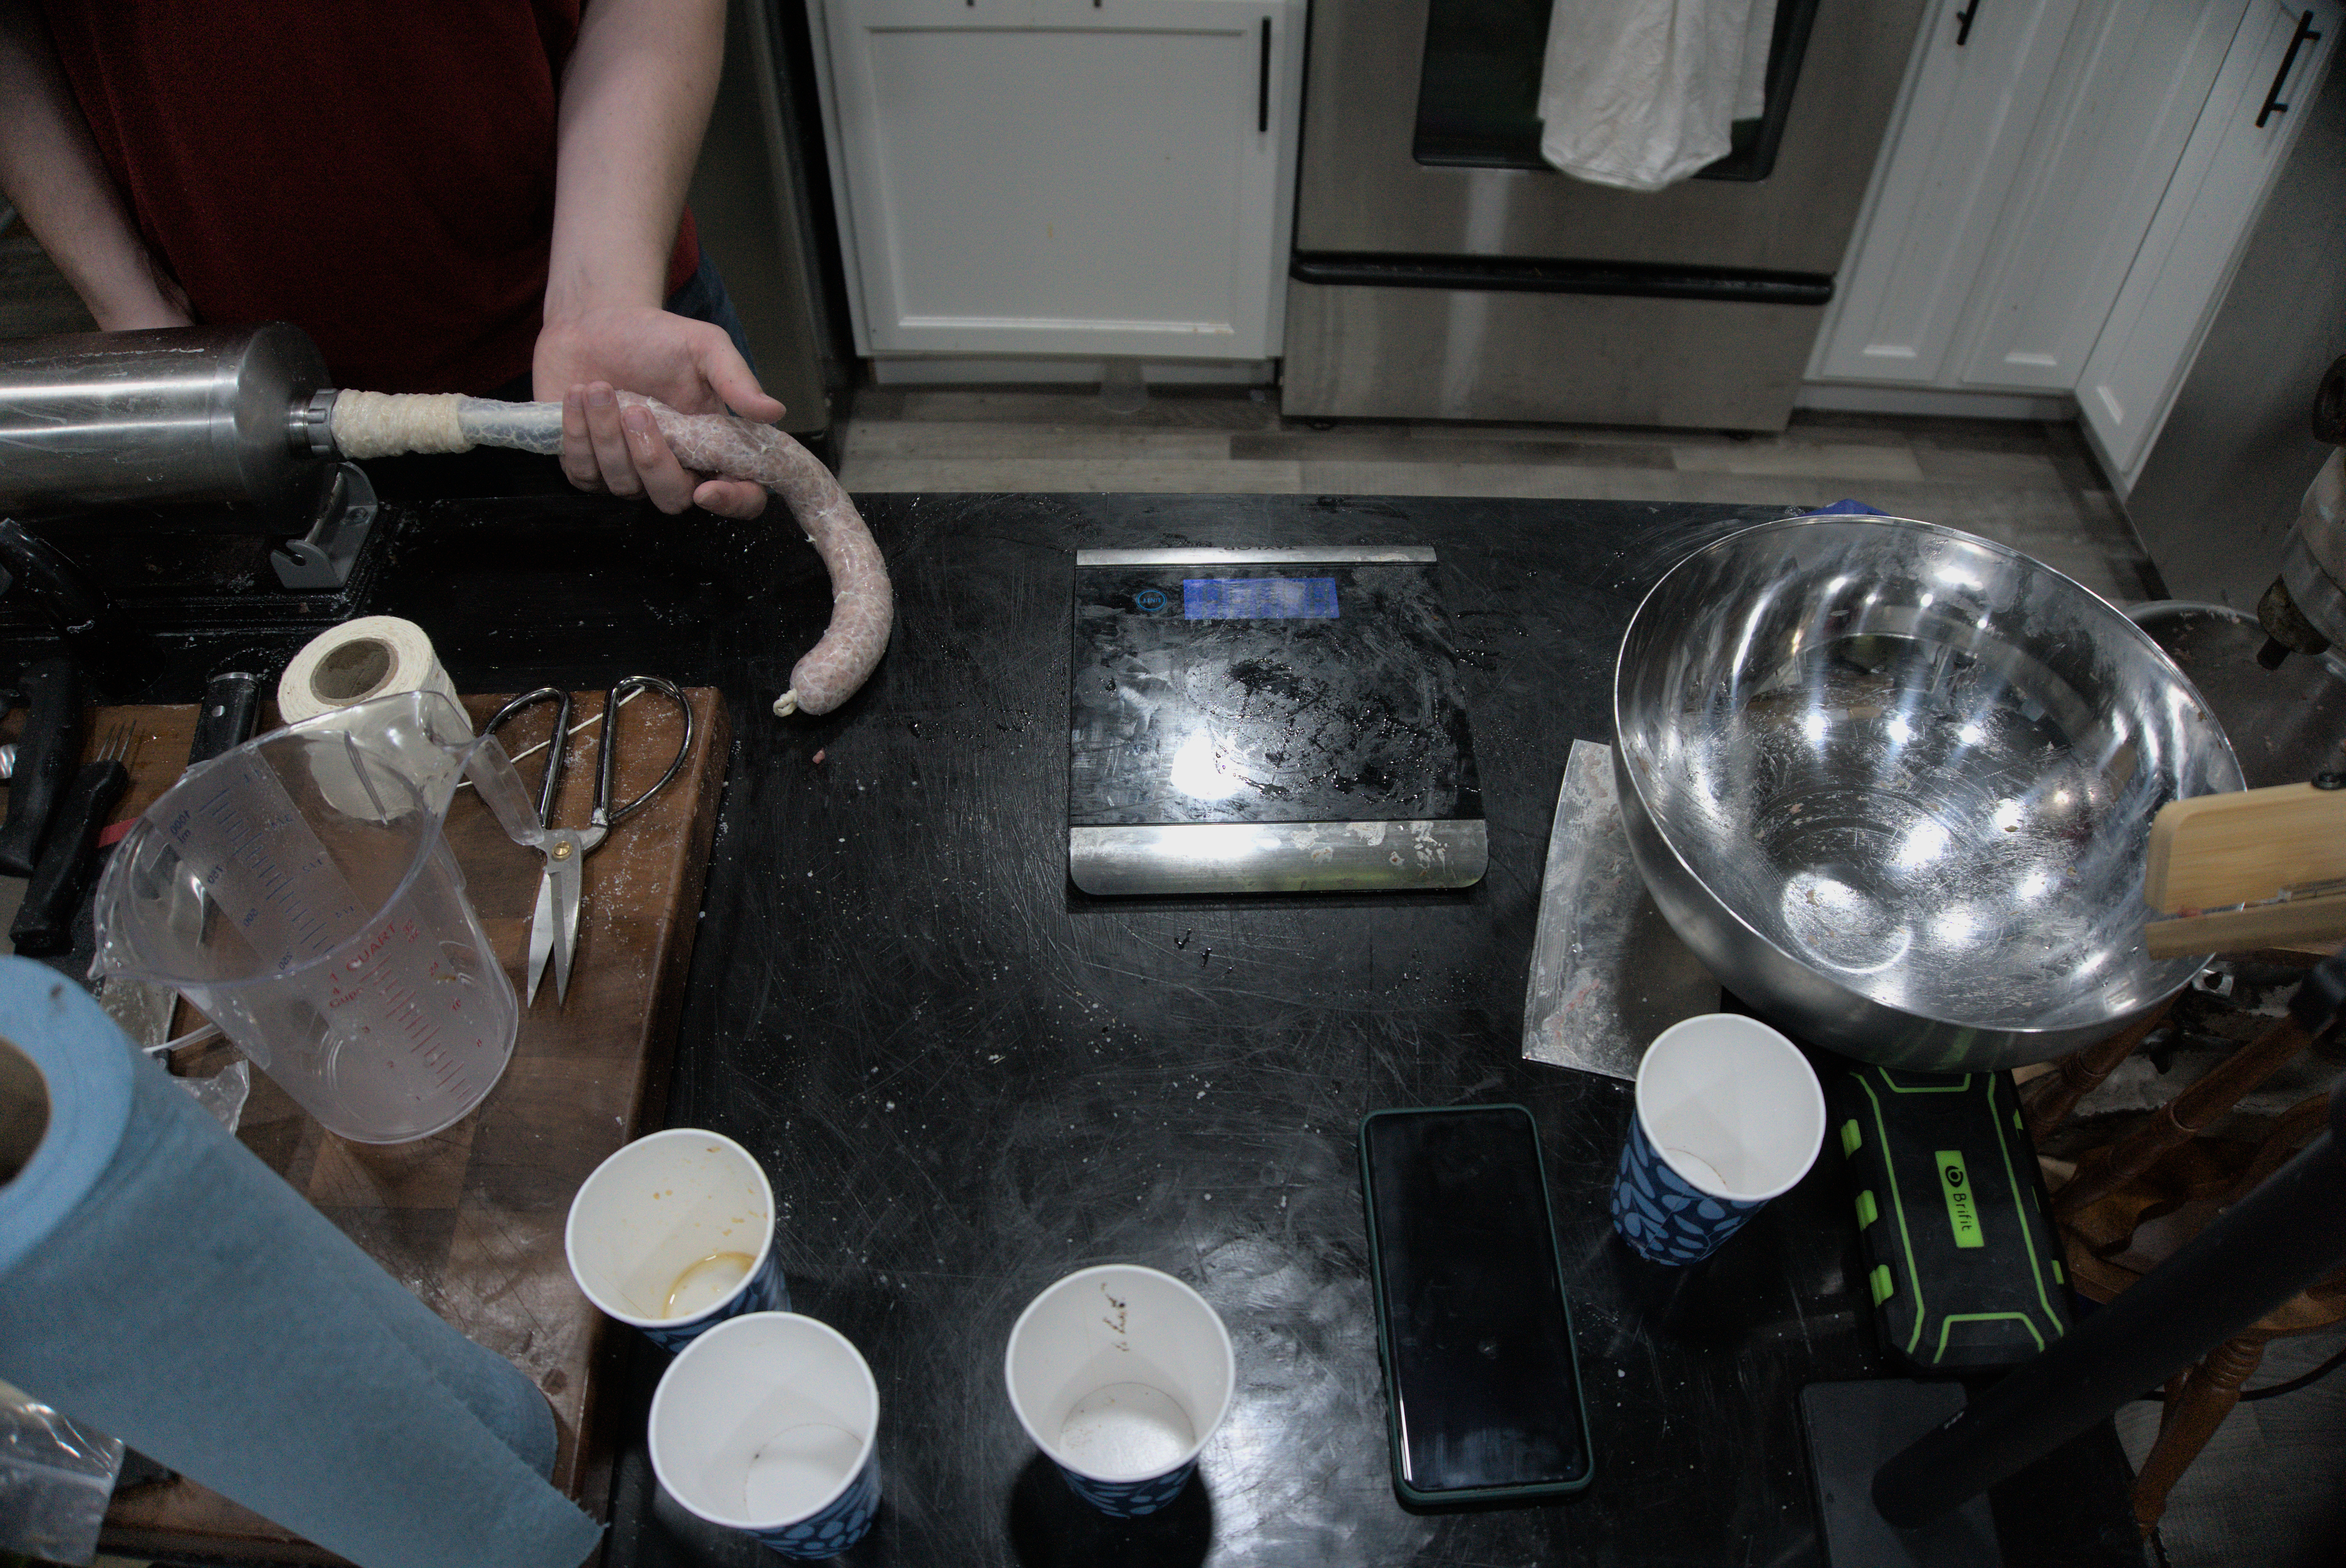
\includegraphics[width=0.9\textwidth]{Figures/20240524_0124.jpg}
	\caption{[Replace with funnel picture]}
	\label{stuffer}
\end{figure}

\subsubsection{Casings}

The casings that I used were both from the the Sausage Maker company. The Natural casings I used were hog casings\footnote{https://www.sausagemaker.com/product/natural-hog-casings-29-32mm/}.

\subsubsection{Drying}

For the dried sausage I hung them in my curing chamber. This chamber is designed to mimic the conditions found in cellars and storage rooms used in period. It is a converted old upright freezer which had humidifiers and dehumidifiers to maintain a relatively consistent 50-55F\textdegree and 75-80\% humidity. At the beginning of the process I measured the weight of each sausage and labeled them. Once they reached 30\% weight loss from their initial marked weight they are considered done.

\FloatBarrier

\subsection{Making Bacon}

The main process that was used for making the bacon was salt curing. I then split the pork belly in half after five days, left half in the salt and moved the other half into the curing/drying chamber. Finally, I took half of each version right before Pennsic and cold smoked them with the sausages for a couple hours.

\subsubsection{Salt Curing}
I used sea salt to cure the pork belly with the salt box method. I poured ~25lbs of salt into the bottom a food safe container, added the pork belly, and then added 50lbs of salt on top of it to both cover it and add weight. After 2 days i removed the salt from on top of it, flipped it while checking the progress, and re-buried it in the salt. After 5 days it has gotten firm to the touch (a marker described in period manuscripts). At this point I split the belly in half on its widest axis leaving two squarish sections. One section was re-buried in the salt and the other was transferred into the curing chamber.

\subsubsection{Dry Curing}

The half that was transferred to the curing chamber was left until it was time for Pennsic (~1 month) and then split again where half was smoked and then both were vacuum sealed to maintain moisture content.

\subsubsection{Smoking}

Half of each salt cured and dry cured halves of the pork belly were cold smoked with the smoked sausages right before Pennsic in the smokehouse.

\subsection{Differences from Period}

\subsubsection{Safety} In order to make sure that the sausages were safe I had to make a couple of changes that decreased risk of food poisoning and botulism. The main difference was that the recipes included a small amount of Curing salt \#1 which contains nitrates/ites which inhibit/reduce the growth of bad bacterial and fungi. In a previous A\&S competition i did some comparisons between using curing salt and not using it and there was no noticeable flavor difference. Especially with strongly flavored and smoke sausages. 

I also sous vide the fresh sausage in vacuum sealed bags to essentially pasteurize the sausage in the bags. This was done at 150F\textdegree for over two hours to ensure the sausages were at temperature for more than 30 minutes (the required time to ensure all bacteria are killed at 140F\textdegree).

For the dry cured sausages I used Curing salt \#2 since they will be hanging for a bit longer. I also brushed their casings with a starter culture of a safe mold used in sausage making to ensure only that grew on them. This should reduce the chances of bad mold growing on them.

\subsubsection{Pork} I used modern pork for these recipes. There was some difference in the pigs of period to our modern pigs today. The main difference being that pigs today have been bred with Asian pigs around the 1800s. This introduced a higher resistance to parasites as well as shorter legs. The fat content might also be a bit different today since most modern pigs are bred to be a bit more on the lean side.

\subsubsection{Smoking} I was smoking in a smokehouse. The Smokehouse used had an offset firebox which allowed for smoke to pass through without excess heat. This matches some historic designs. Either for smokehouses or a similar effect to the modified chimney smokers found in some European homes. However the exact design of the smokehouse is a bit more modern in materials.

\bibliography{bibliography.bib}

\FloatBarrier

\section{Illuminations}\label{b:appendix2}

\begin{figure}[!htb]
	\centering
	\includegraphics[width=0.45\textwidth]{Figures/Amb. 317.2° Folio 59 verso (Mendel I).jpeg}
	\caption{\citep[page 59 Left]{Mendel}}
\end{figure}

\begin{figure}[!htb]
	\centering
	\includegraphics[width=0.45\textwidth]{Figures/Amb. 317.2° Folio 83 verso (Mendel I).jpeg}
	\caption{\citep[page 83 Left]{Mendel}}
\end{figure}

\begin{figure}[!htb]
	\centering
	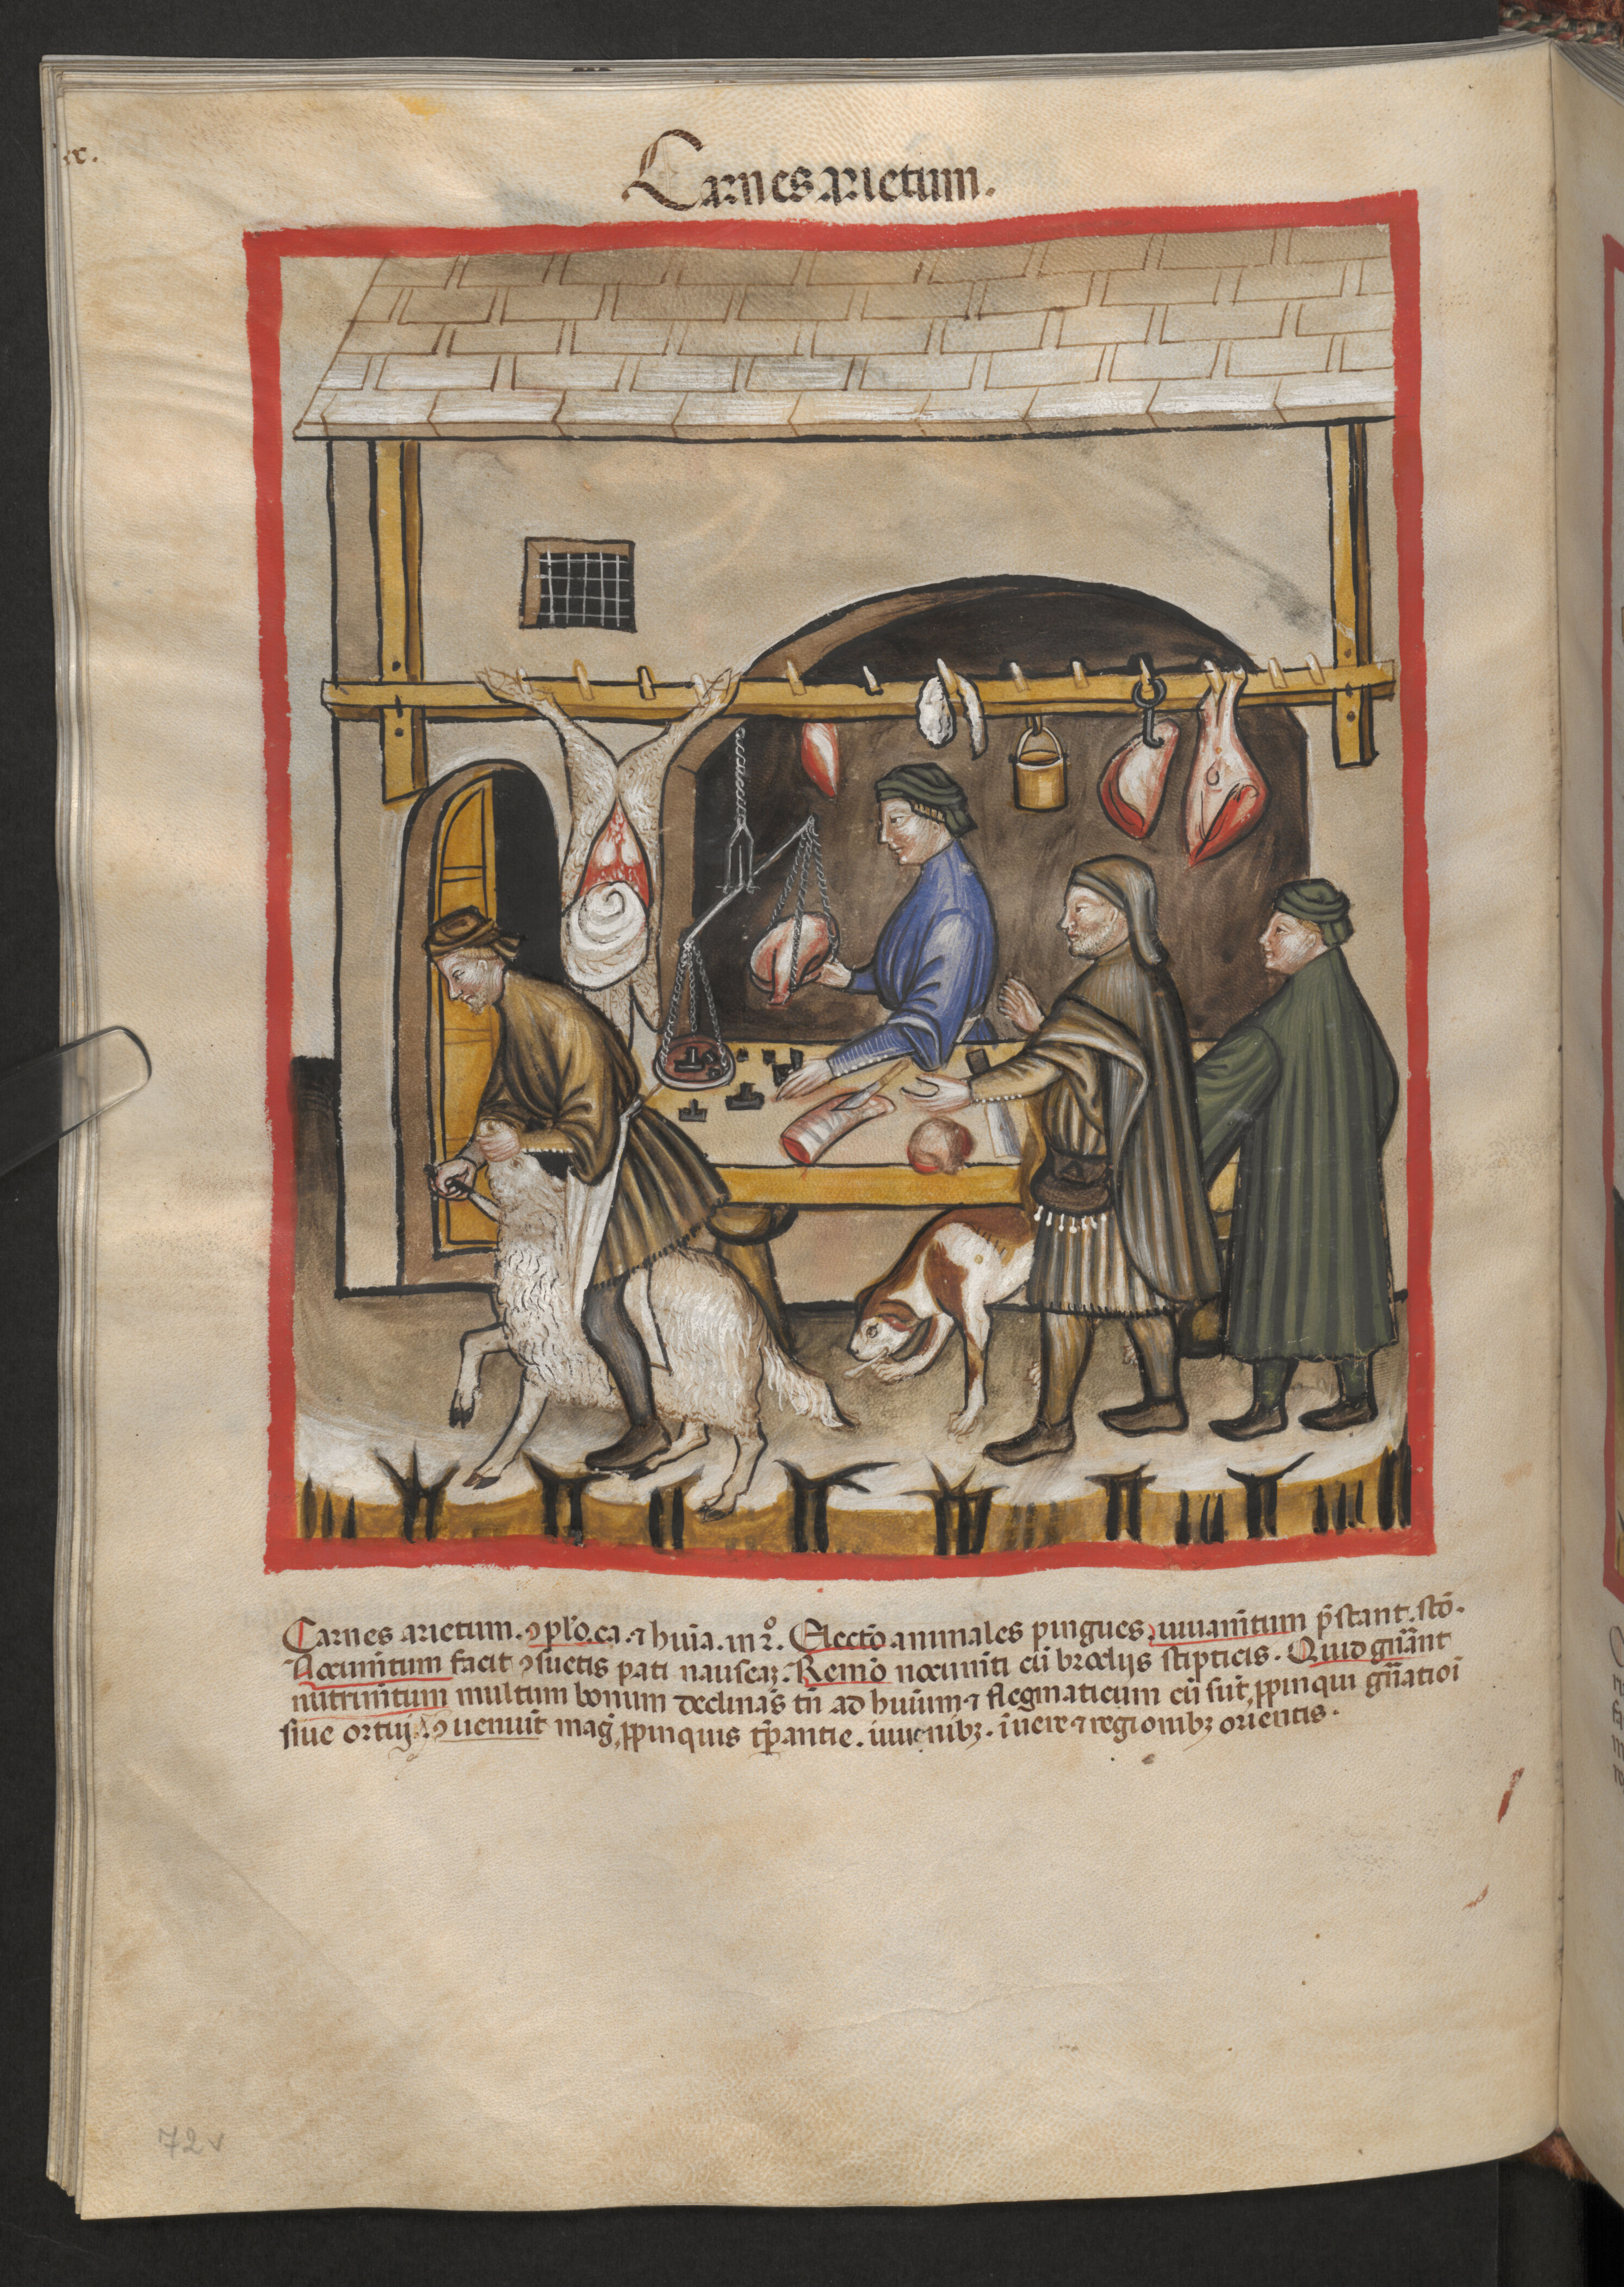
\includegraphics[width=0.45\textwidth]{Figures/Tacuinum_Sanitatis_p73L.png}
	\caption{\citep[page 73 Left]{TacSan}}
\end{figure}

\begin{figure}[!htb]
	\centering
	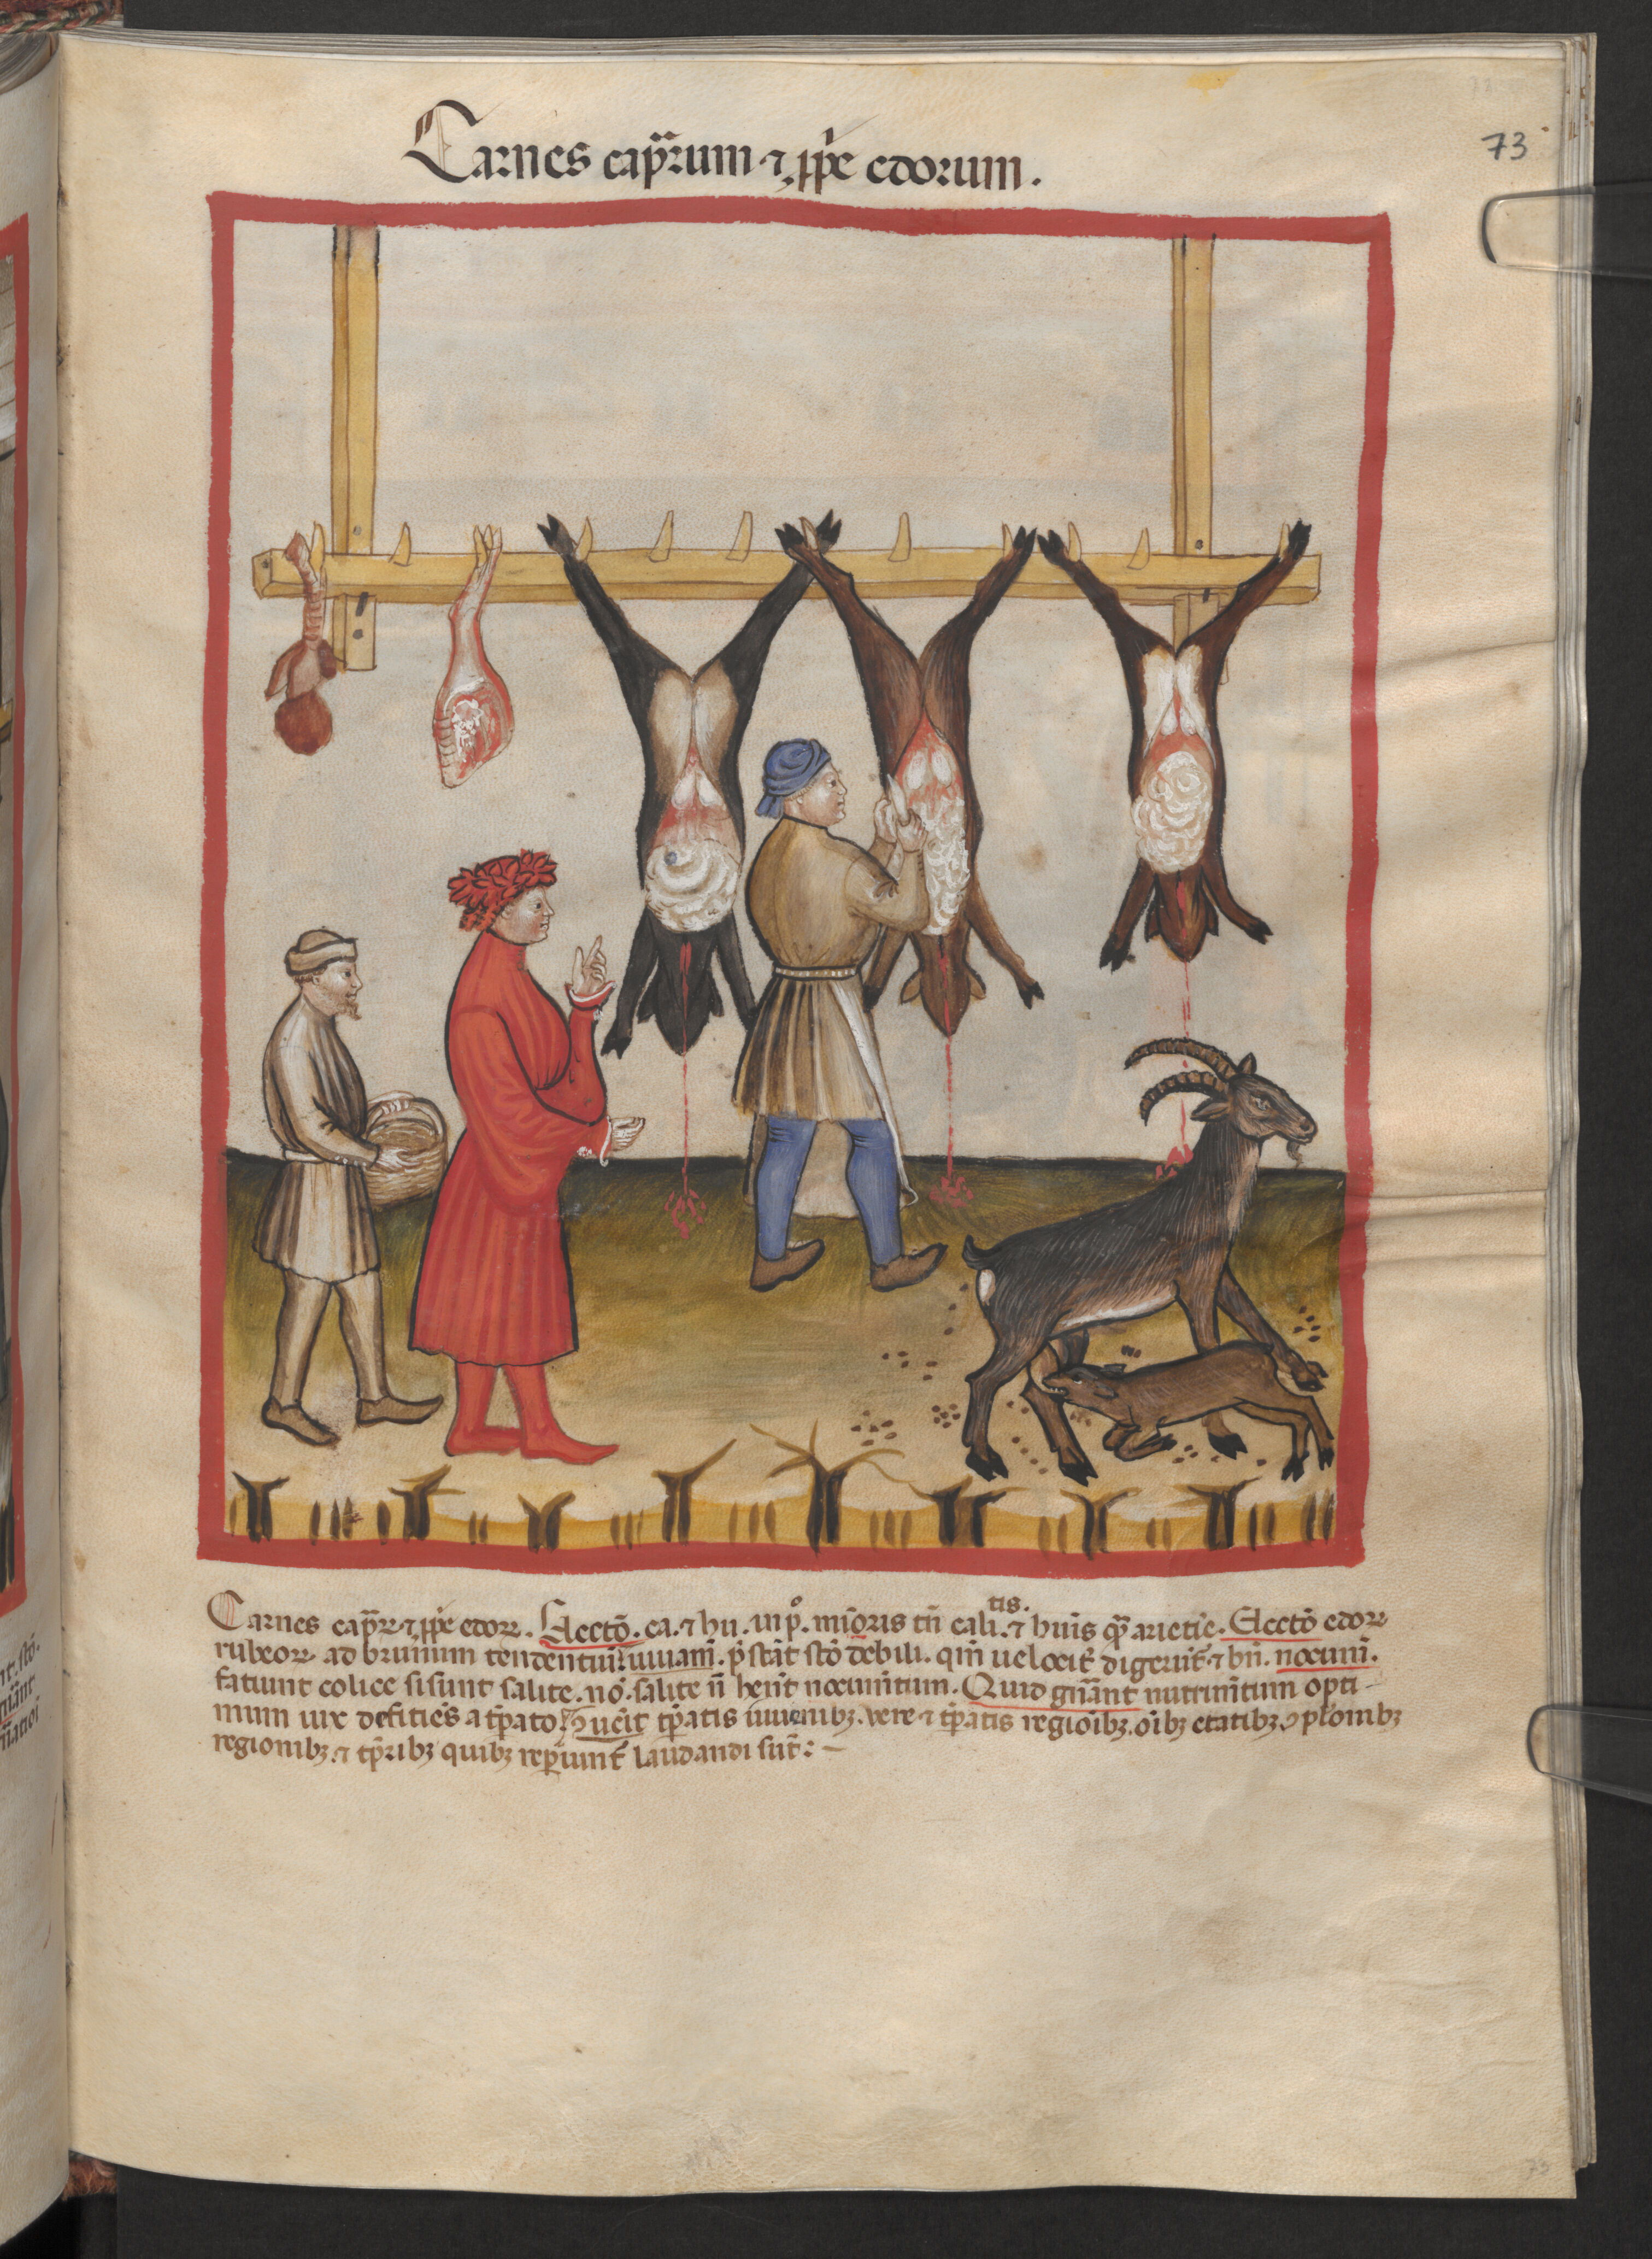
\includegraphics[width=0.45\textwidth]{Figures/Tacuinum_Sanitatis_p73R.png}
	\caption{\citep[page 73 Right]{TacSan}}
\end{figure}

\begin{figure}[!htb]
	\centering
	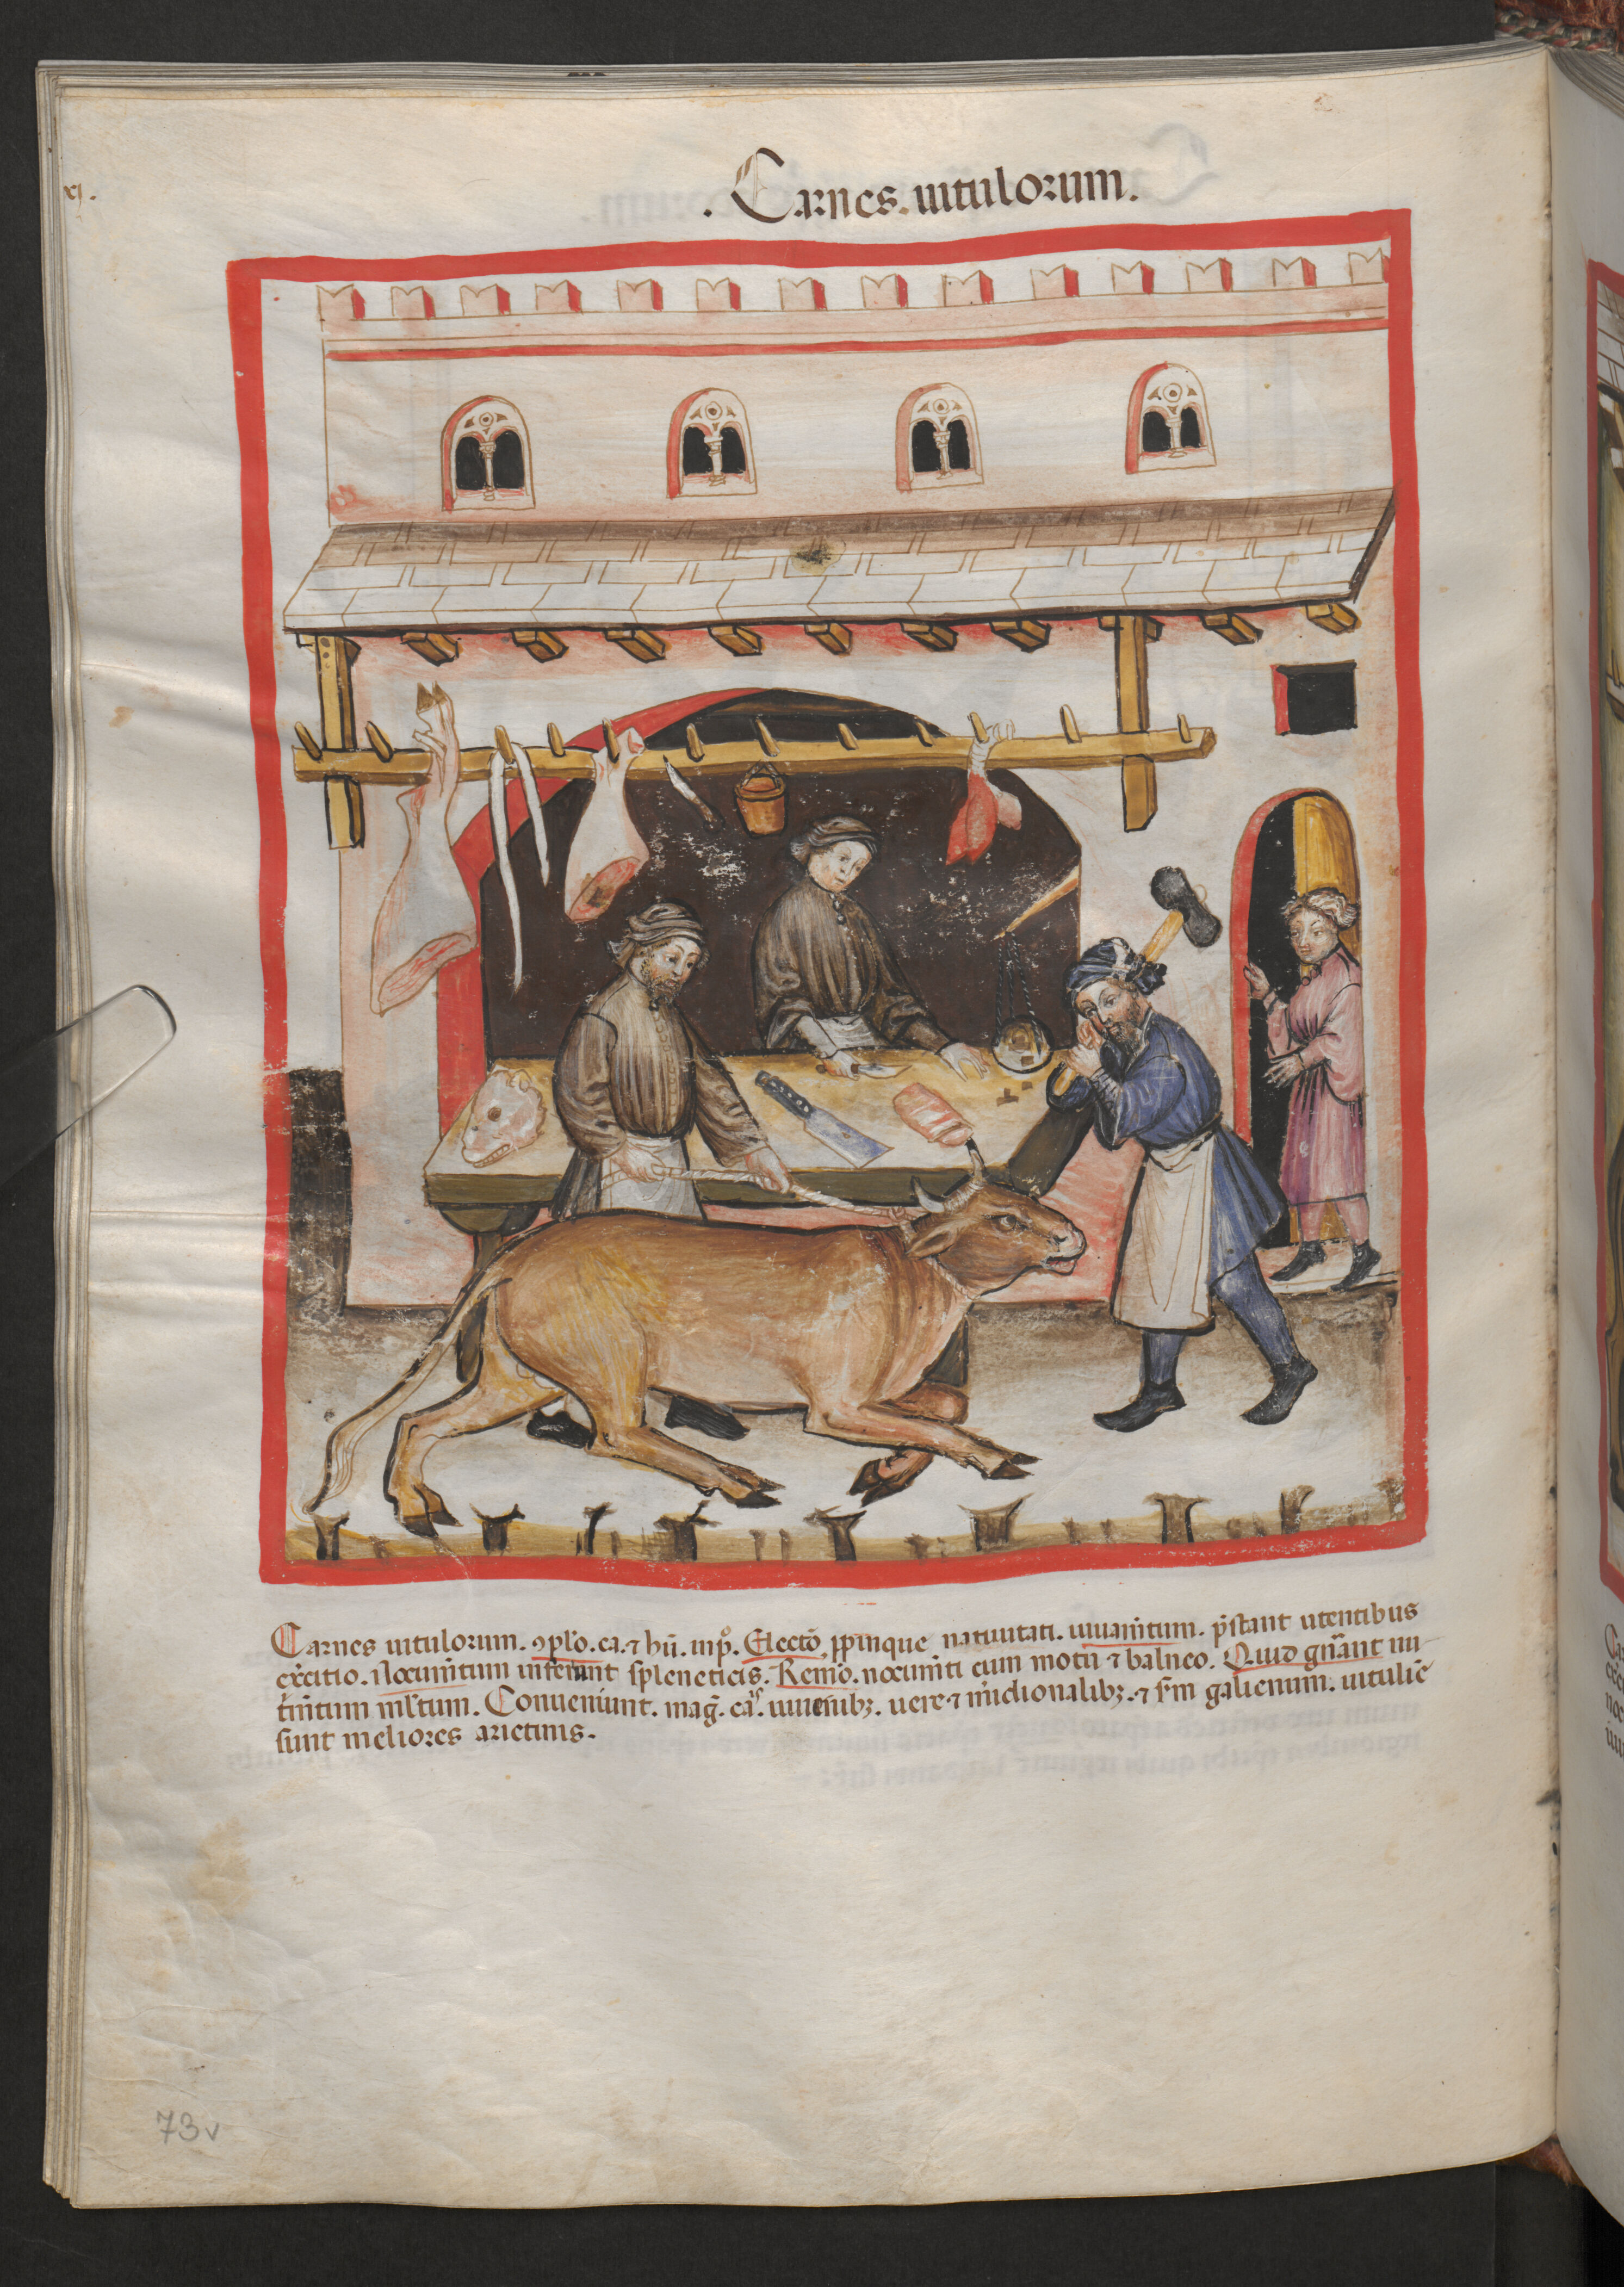
\includegraphics[width=0.45\textwidth]{Figures/Tacuinum_Sanitatis_p74L.png}
	\caption{\citep[page 74 Left]{TacSan}}
\end{figure}

\begin{figure}[!htb]
	\centering
	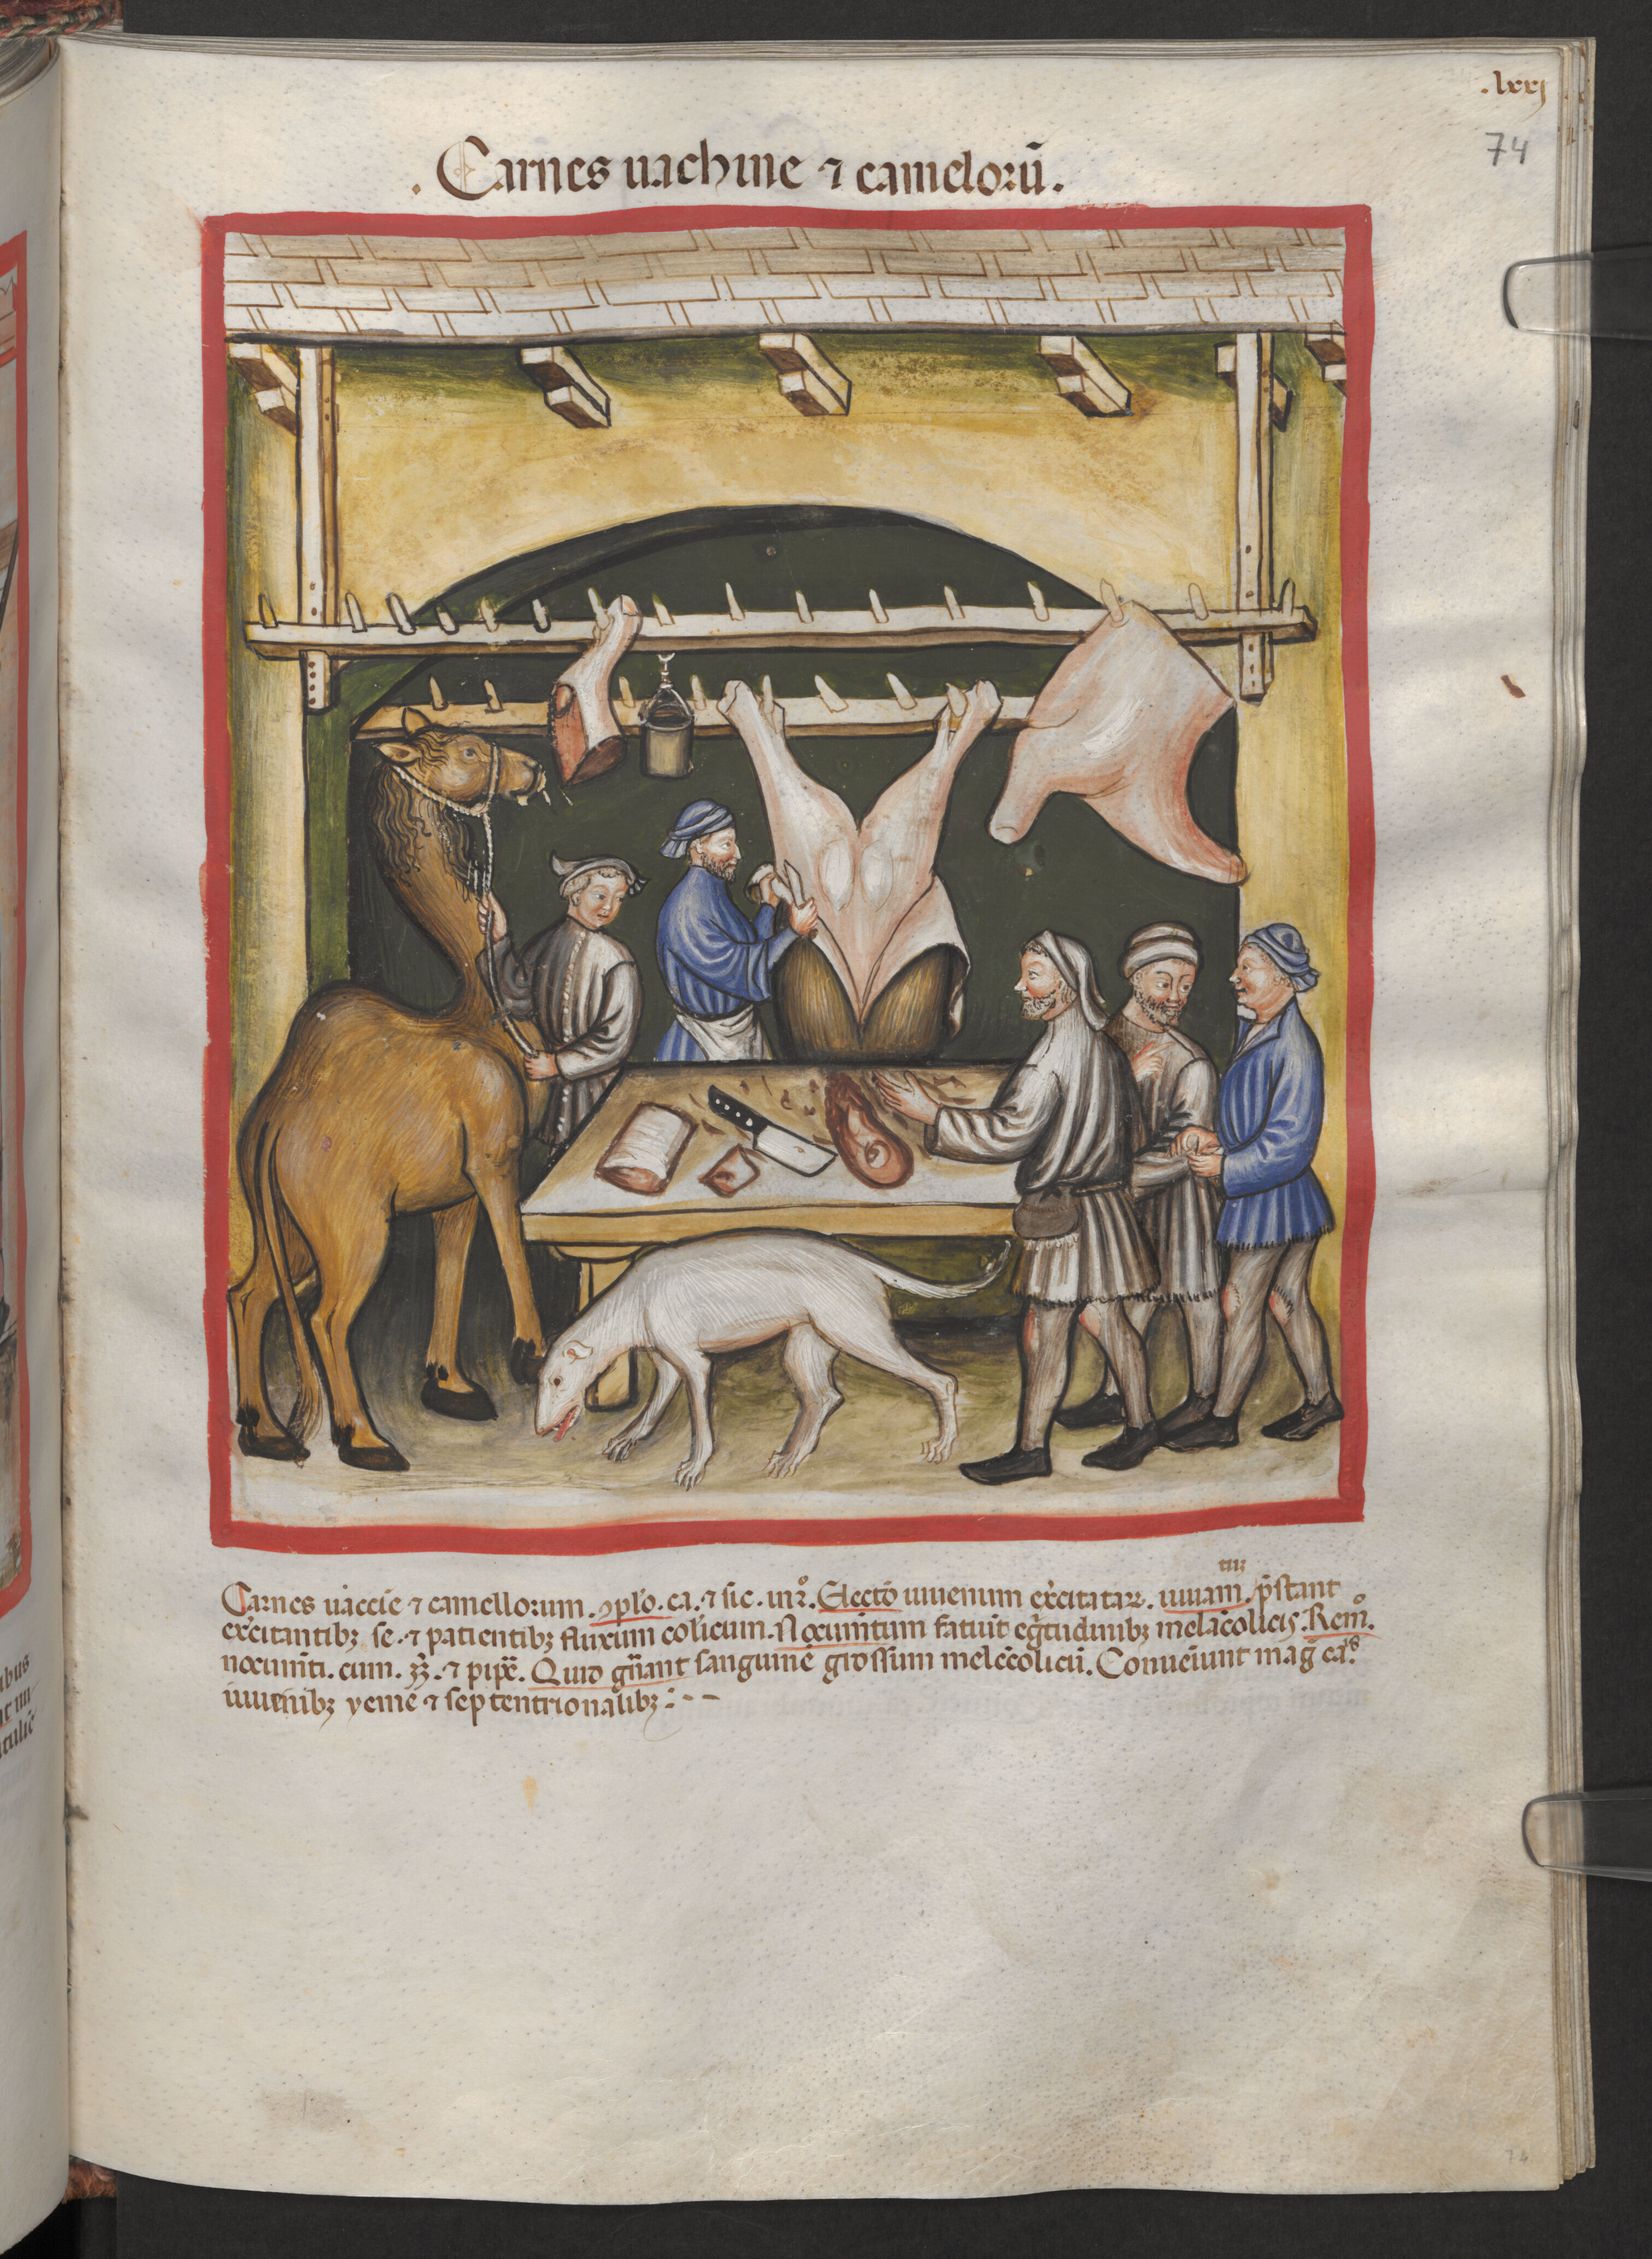
\includegraphics[width=0.45\textwidth]{Figures/Tacuinum_Sanitatis_p74R.png}
	\caption{\citep[page 74 Right]{TacSan}}
\end{figure}

\begin{figure}[!htb]
	\centering
	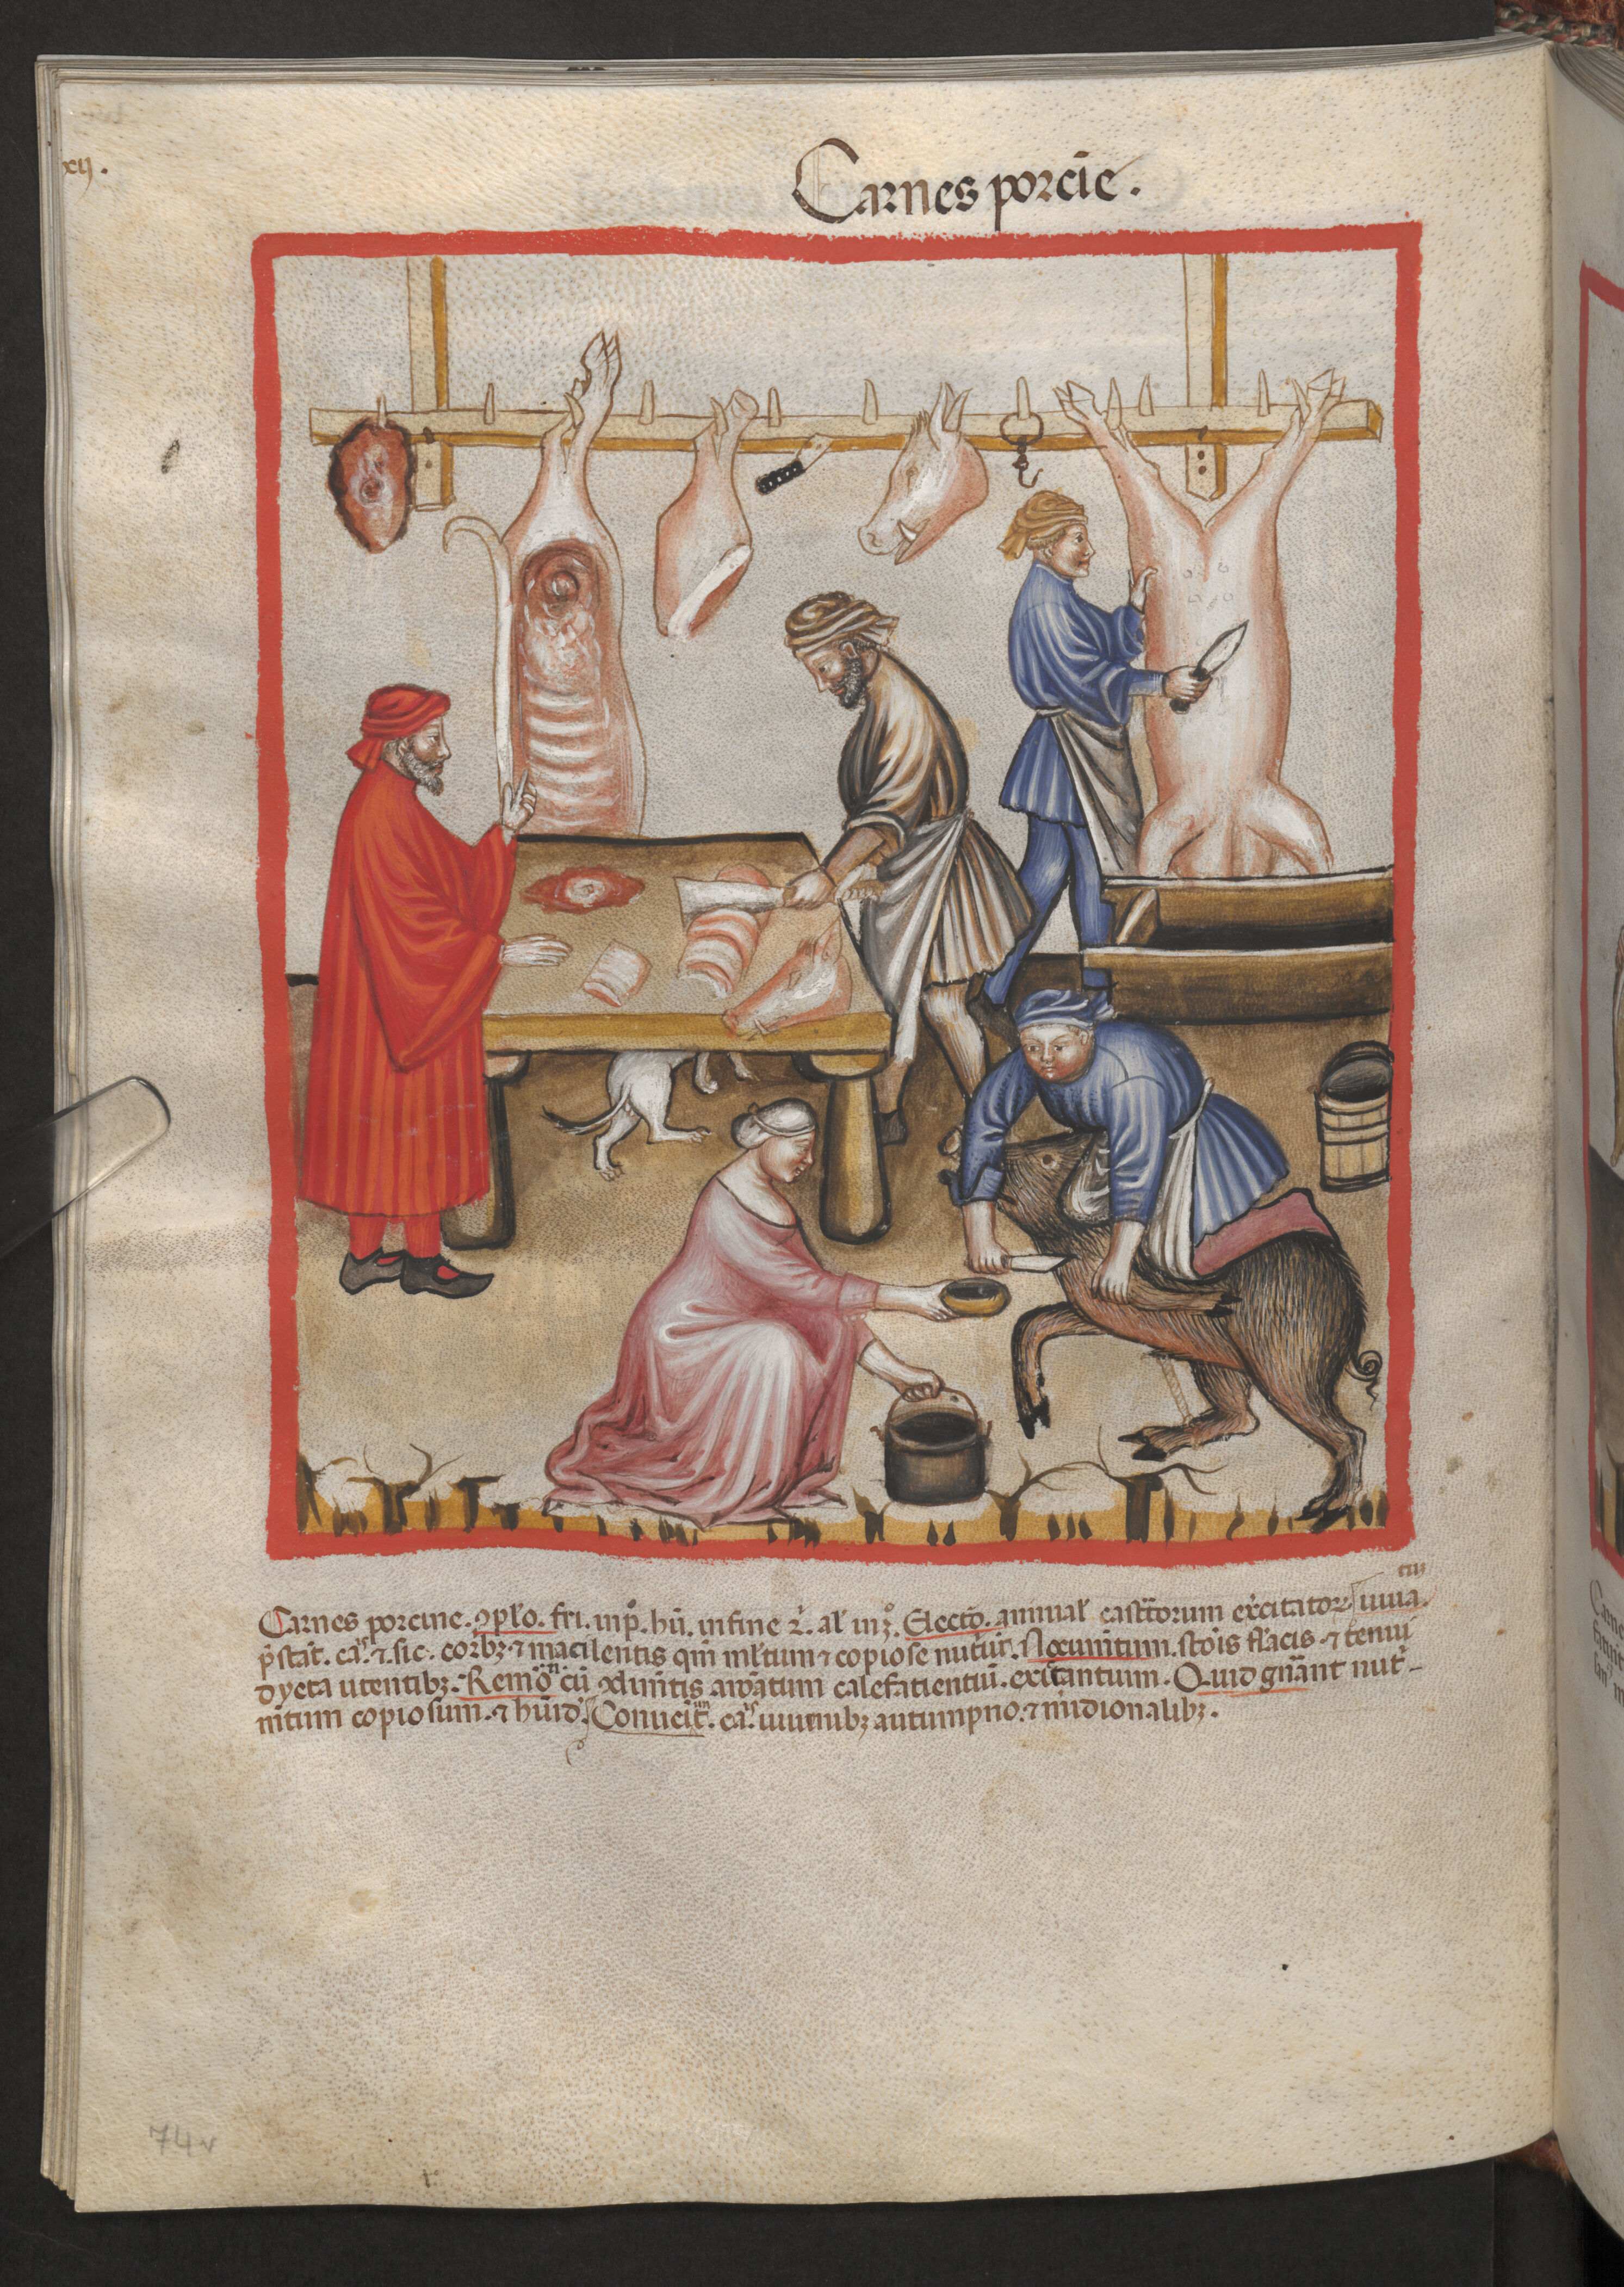
\includegraphics[width=0.45\textwidth]{Figures/Tacuinum_Sanitatis_p75L.png}
	\caption{\citep[page 75 Left]{TacSan}}
\end{figure}

\begin{figure}[!htb]
	\centering
	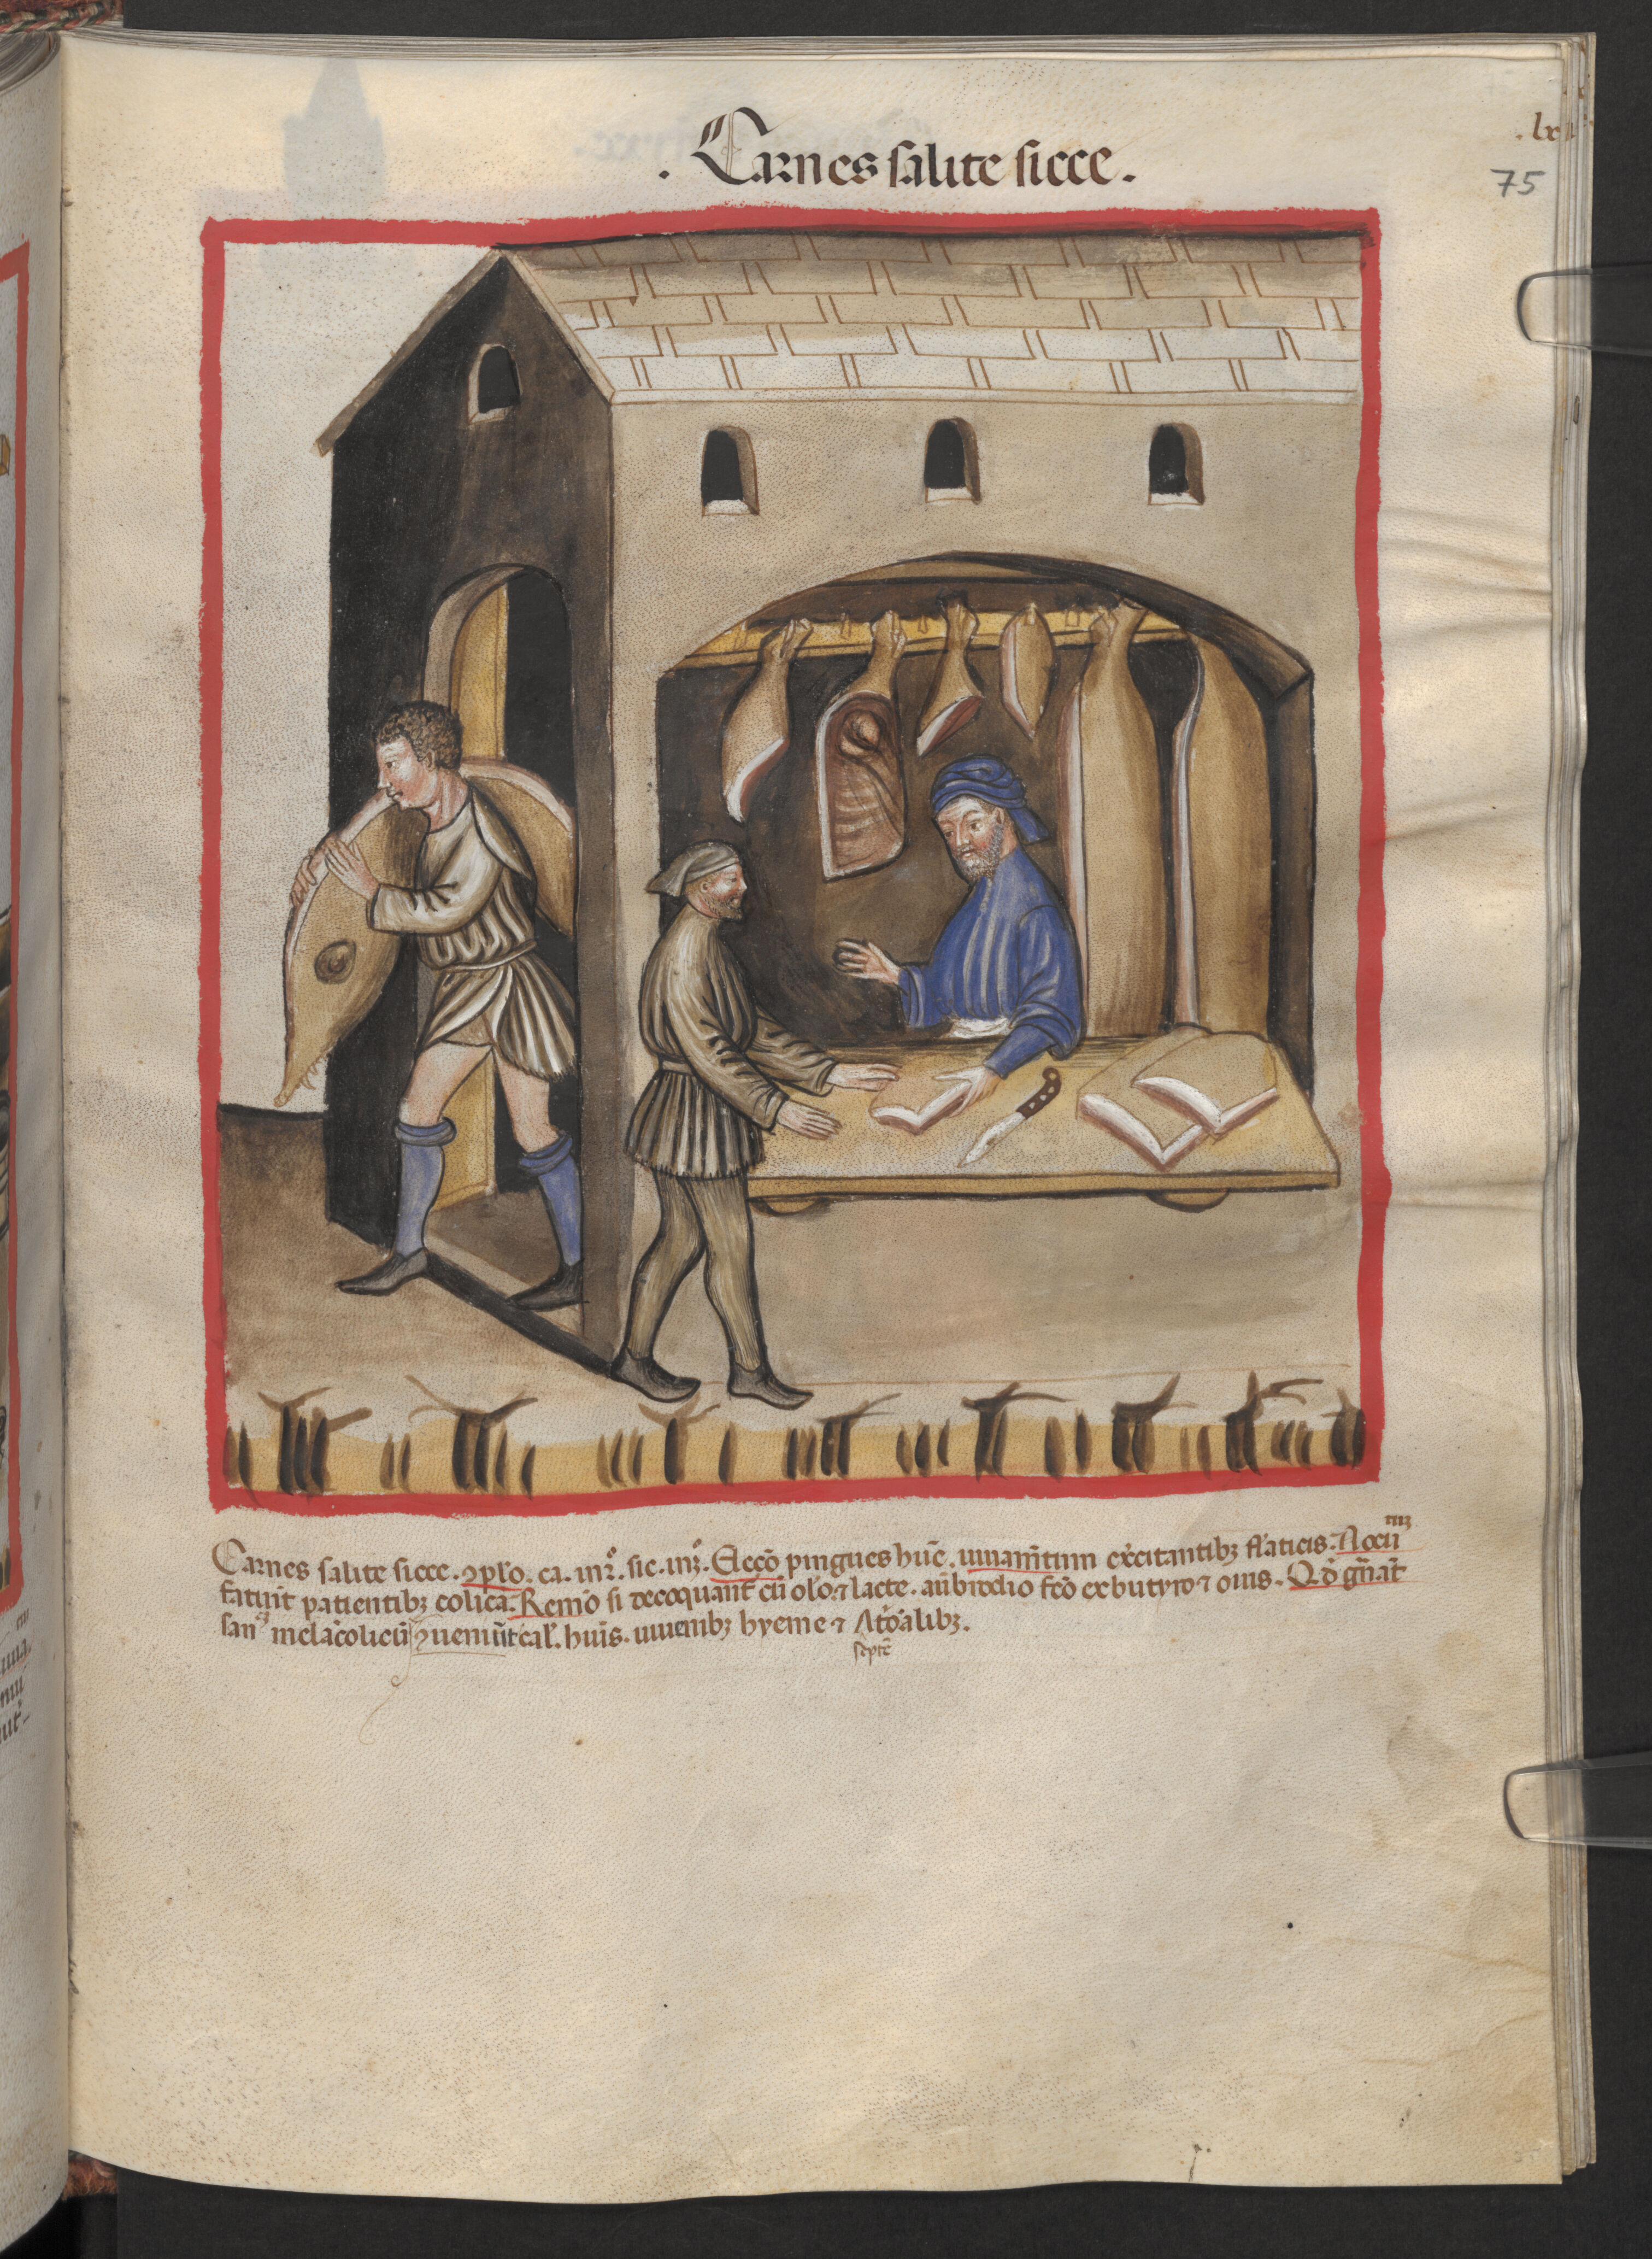
\includegraphics[width=0.45\textwidth]{Figures/Tacuinum_Sanitatis_p75R.png}
	\caption{\citep[page 75 Right]{TacSan}}
\end{figure}

\begin{figure}[!htb]
	\centering
	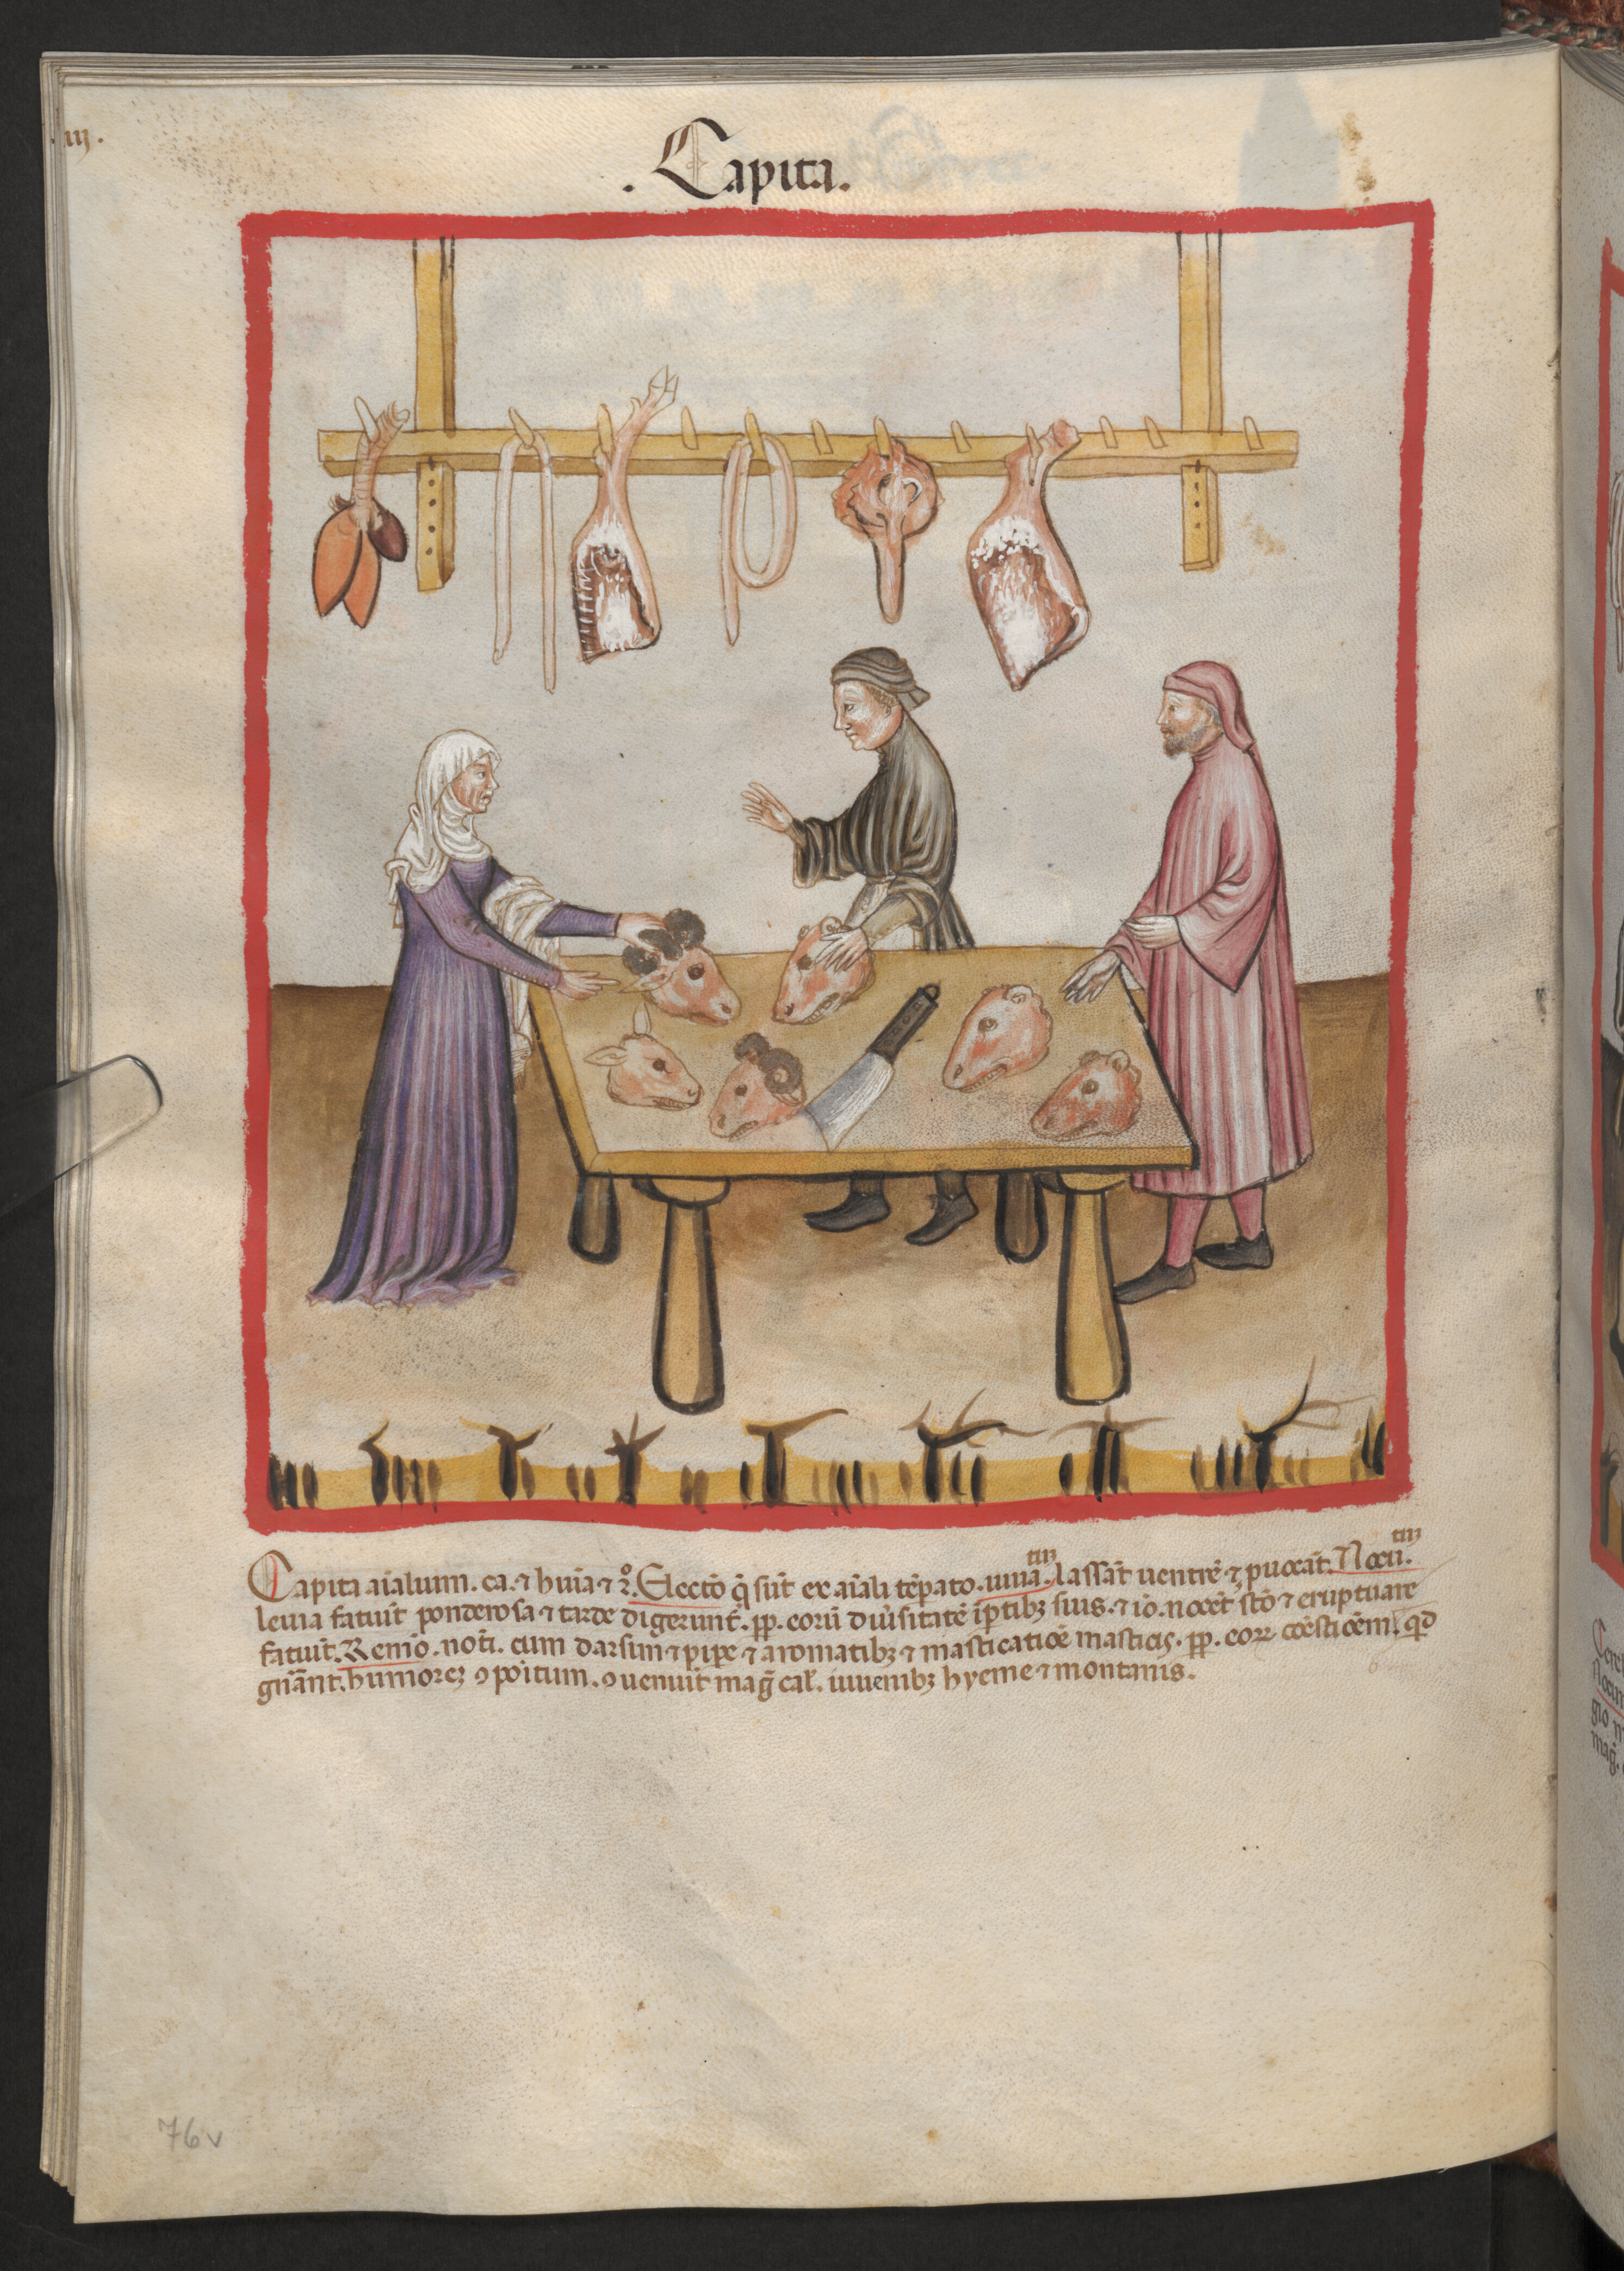
\includegraphics[width=0.45\textwidth]{Figures/Tacuinum_Sanitatis_p77L.png}
	\caption{\citep[page 77 Left]{TacSan}}
\end{figure}

\begin{figure}[!htb]
	\centering
	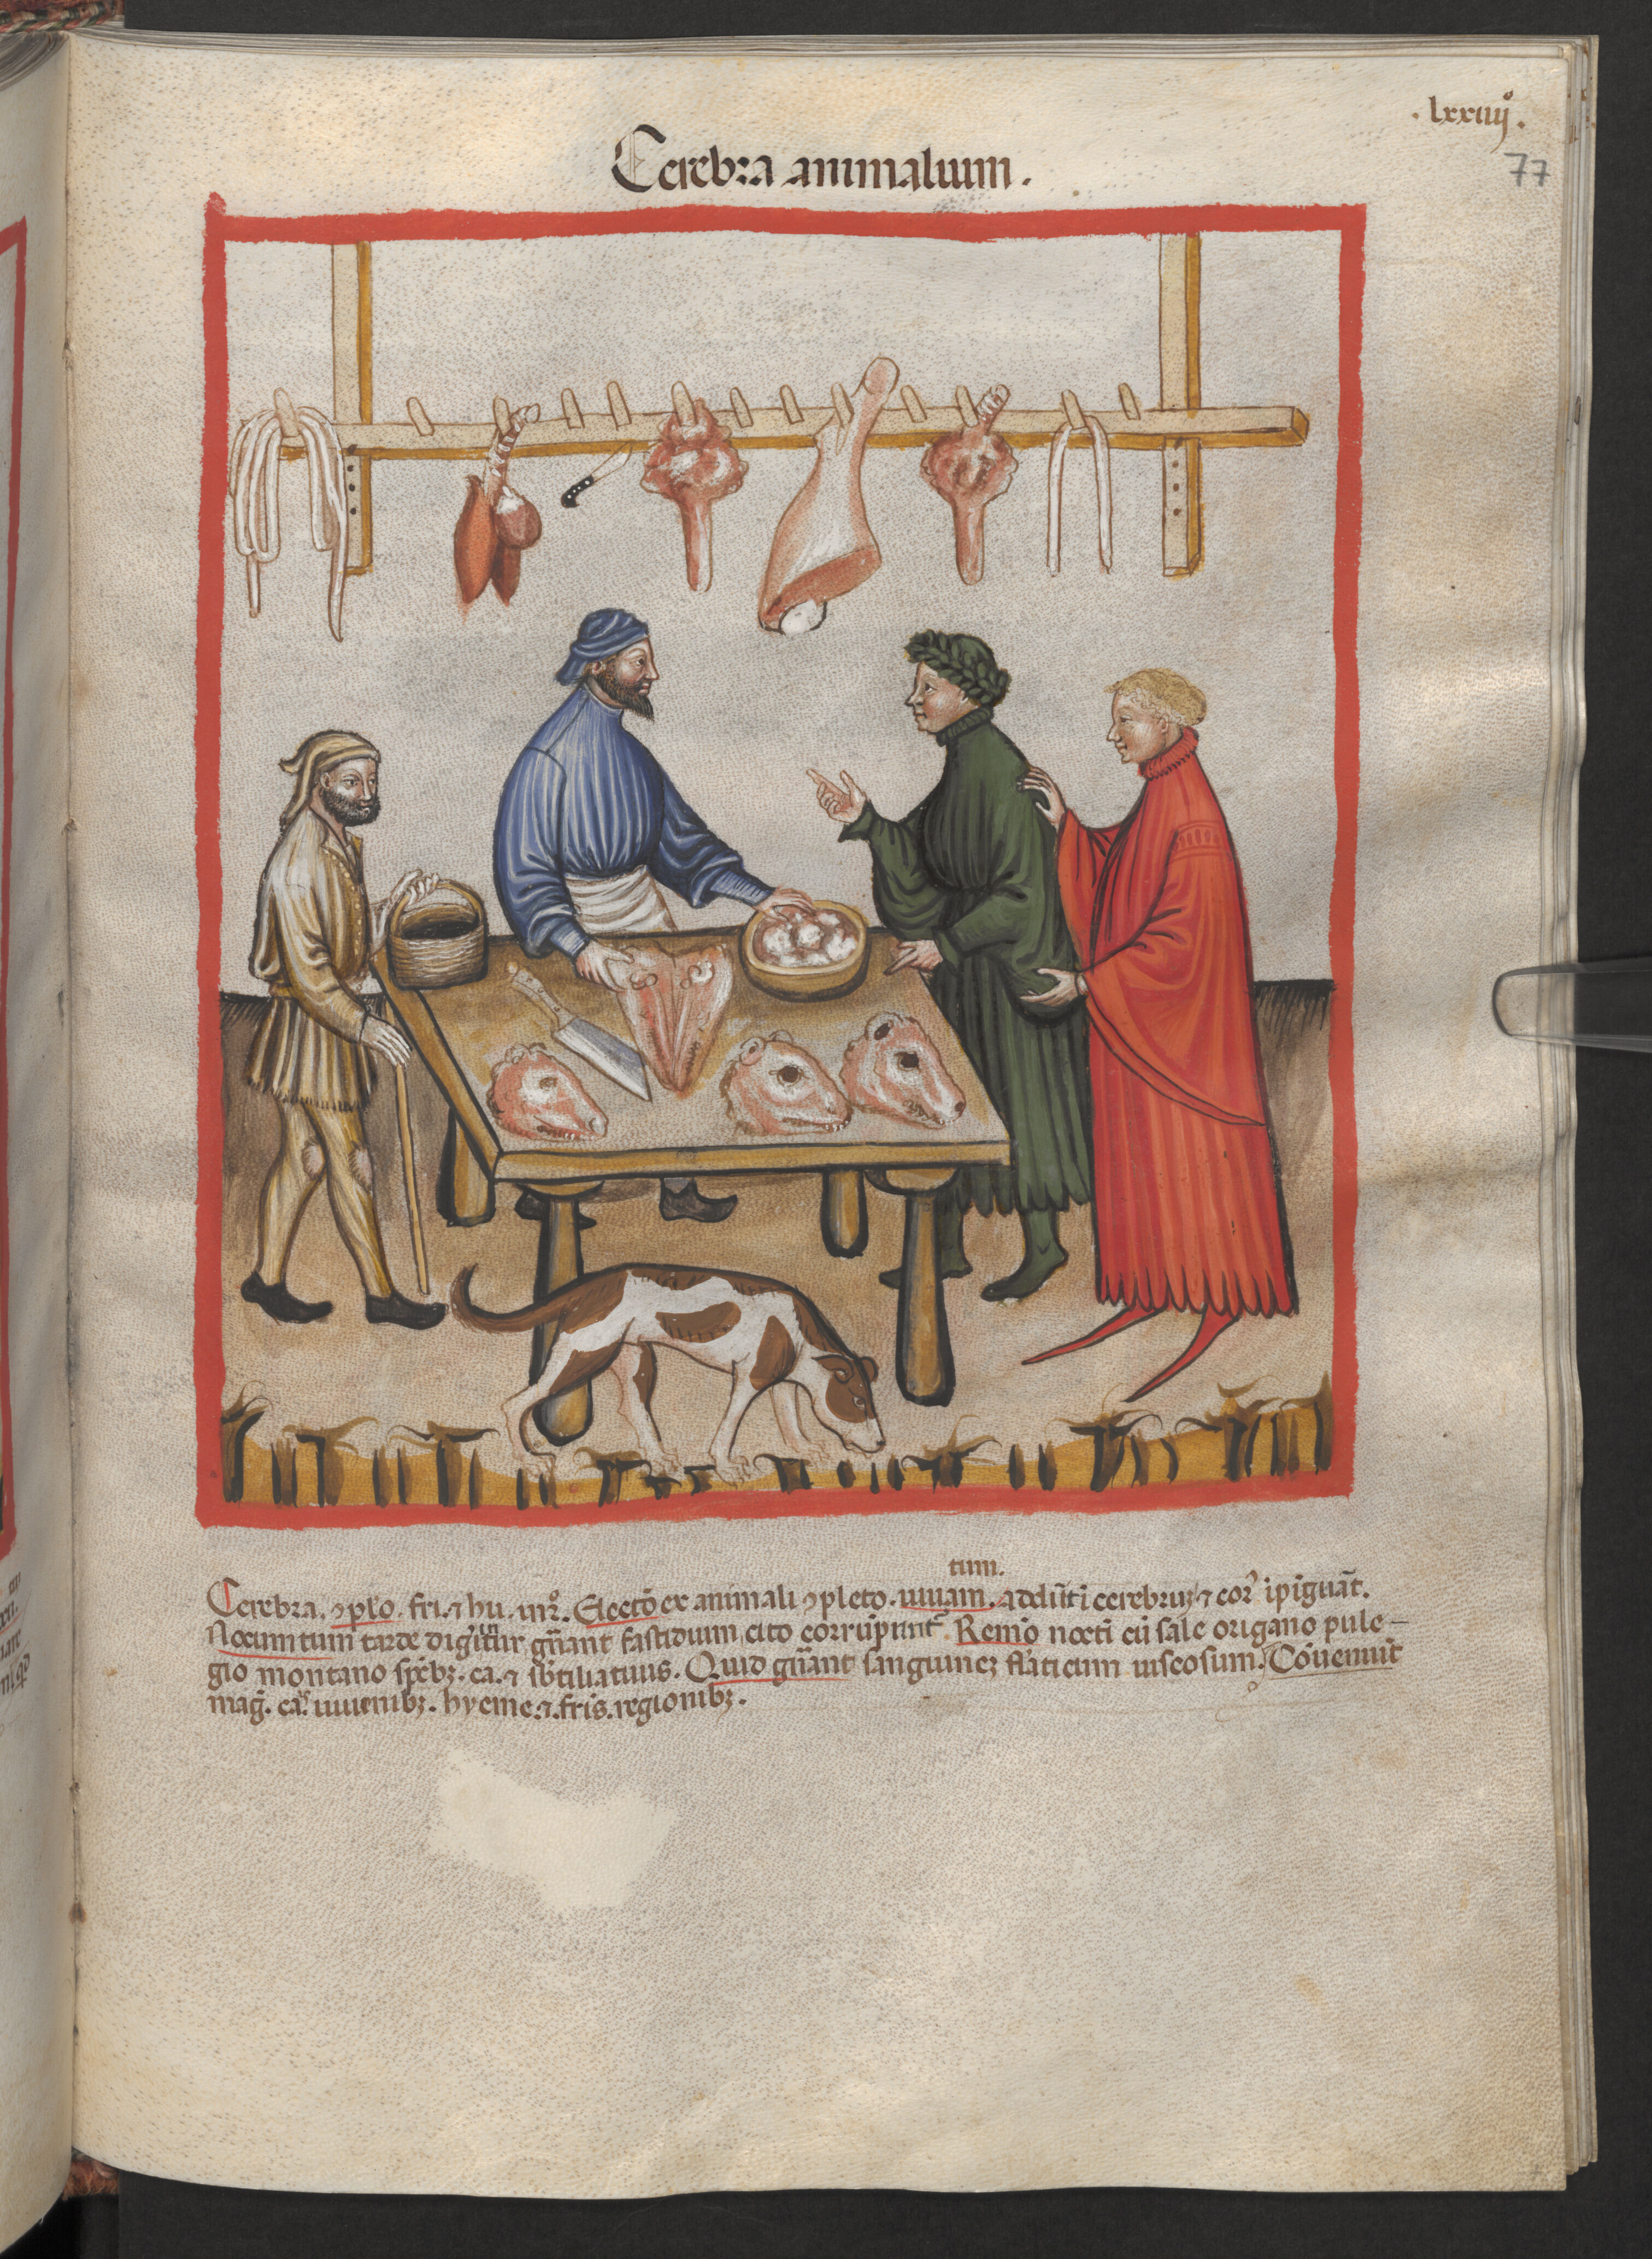
\includegraphics[width=0.45\textwidth]{Figures/Tacuinum_Sanitatis_p77R.png}
	\caption{\citep[page 77 Right]{TacSan}}
\end{figure}

\begin{figure}[!htb]
	\centering
	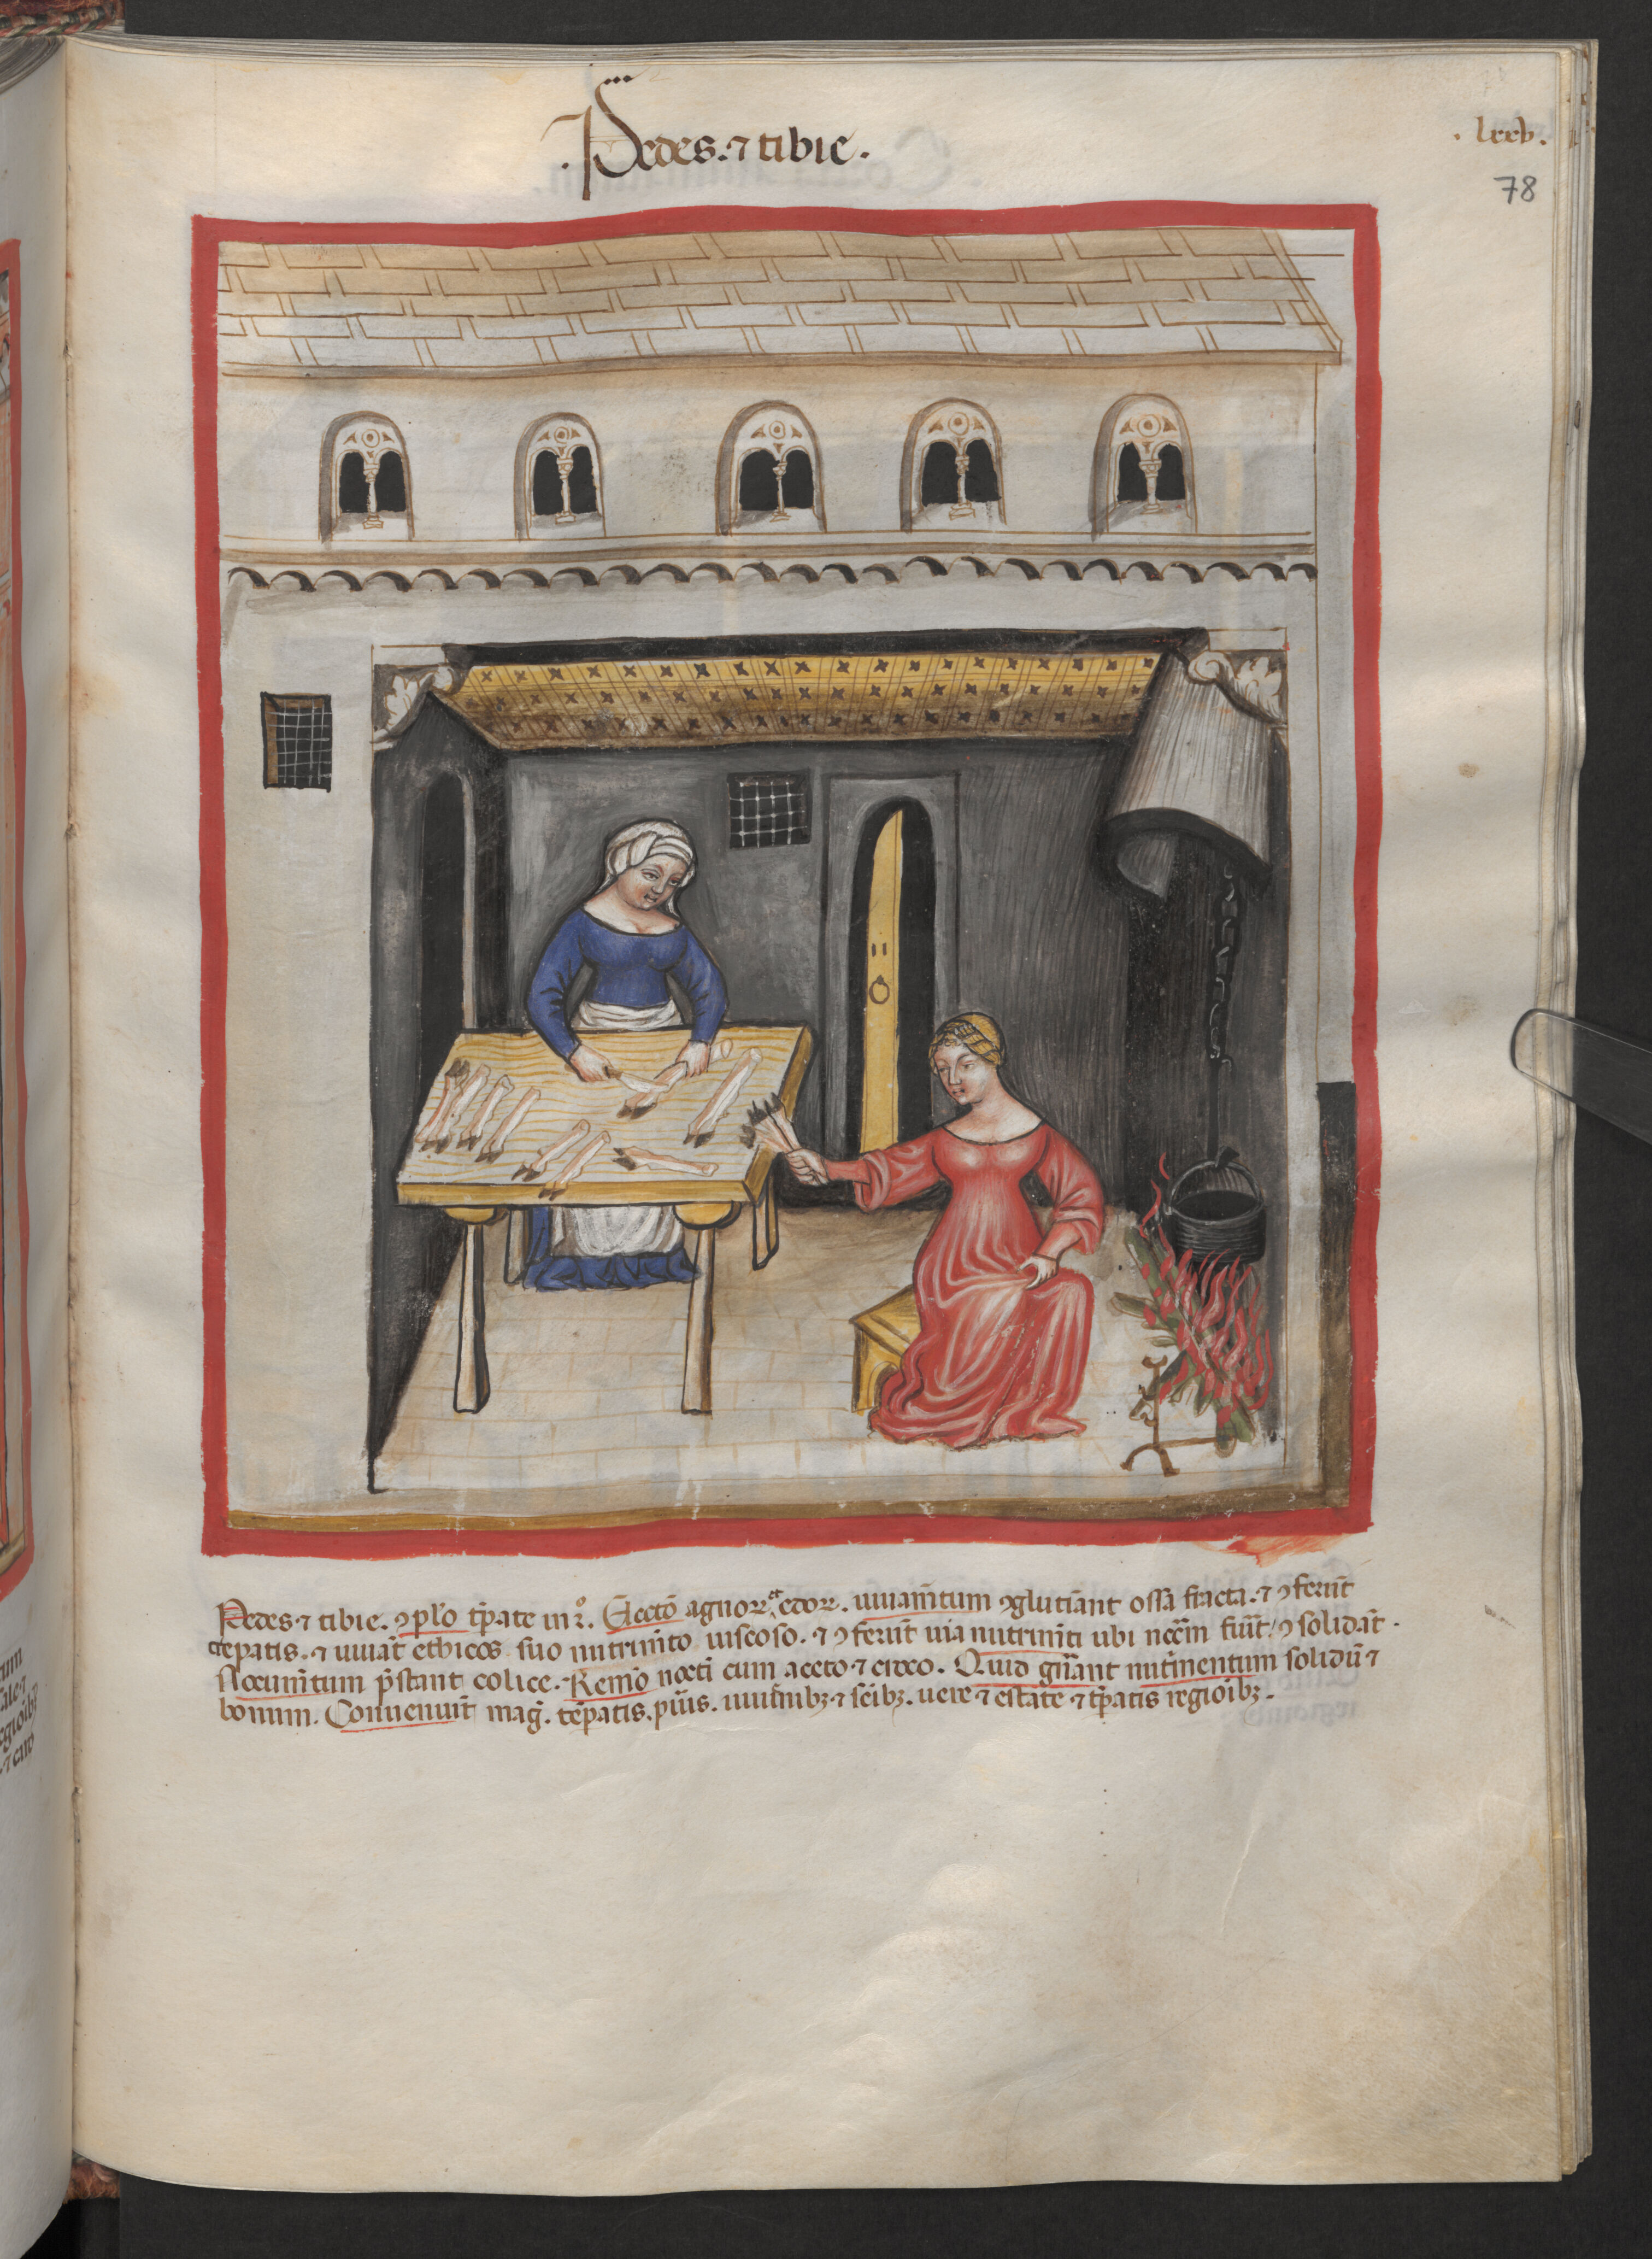
\includegraphics[width=0.45\textwidth]{Figures/Tacuinum_Sanitatis_p78R.png}
	\caption{\citep[page 78 Right]{TacSan}}
\end{figure}

\begin{figure}[!htb]
	\centering
	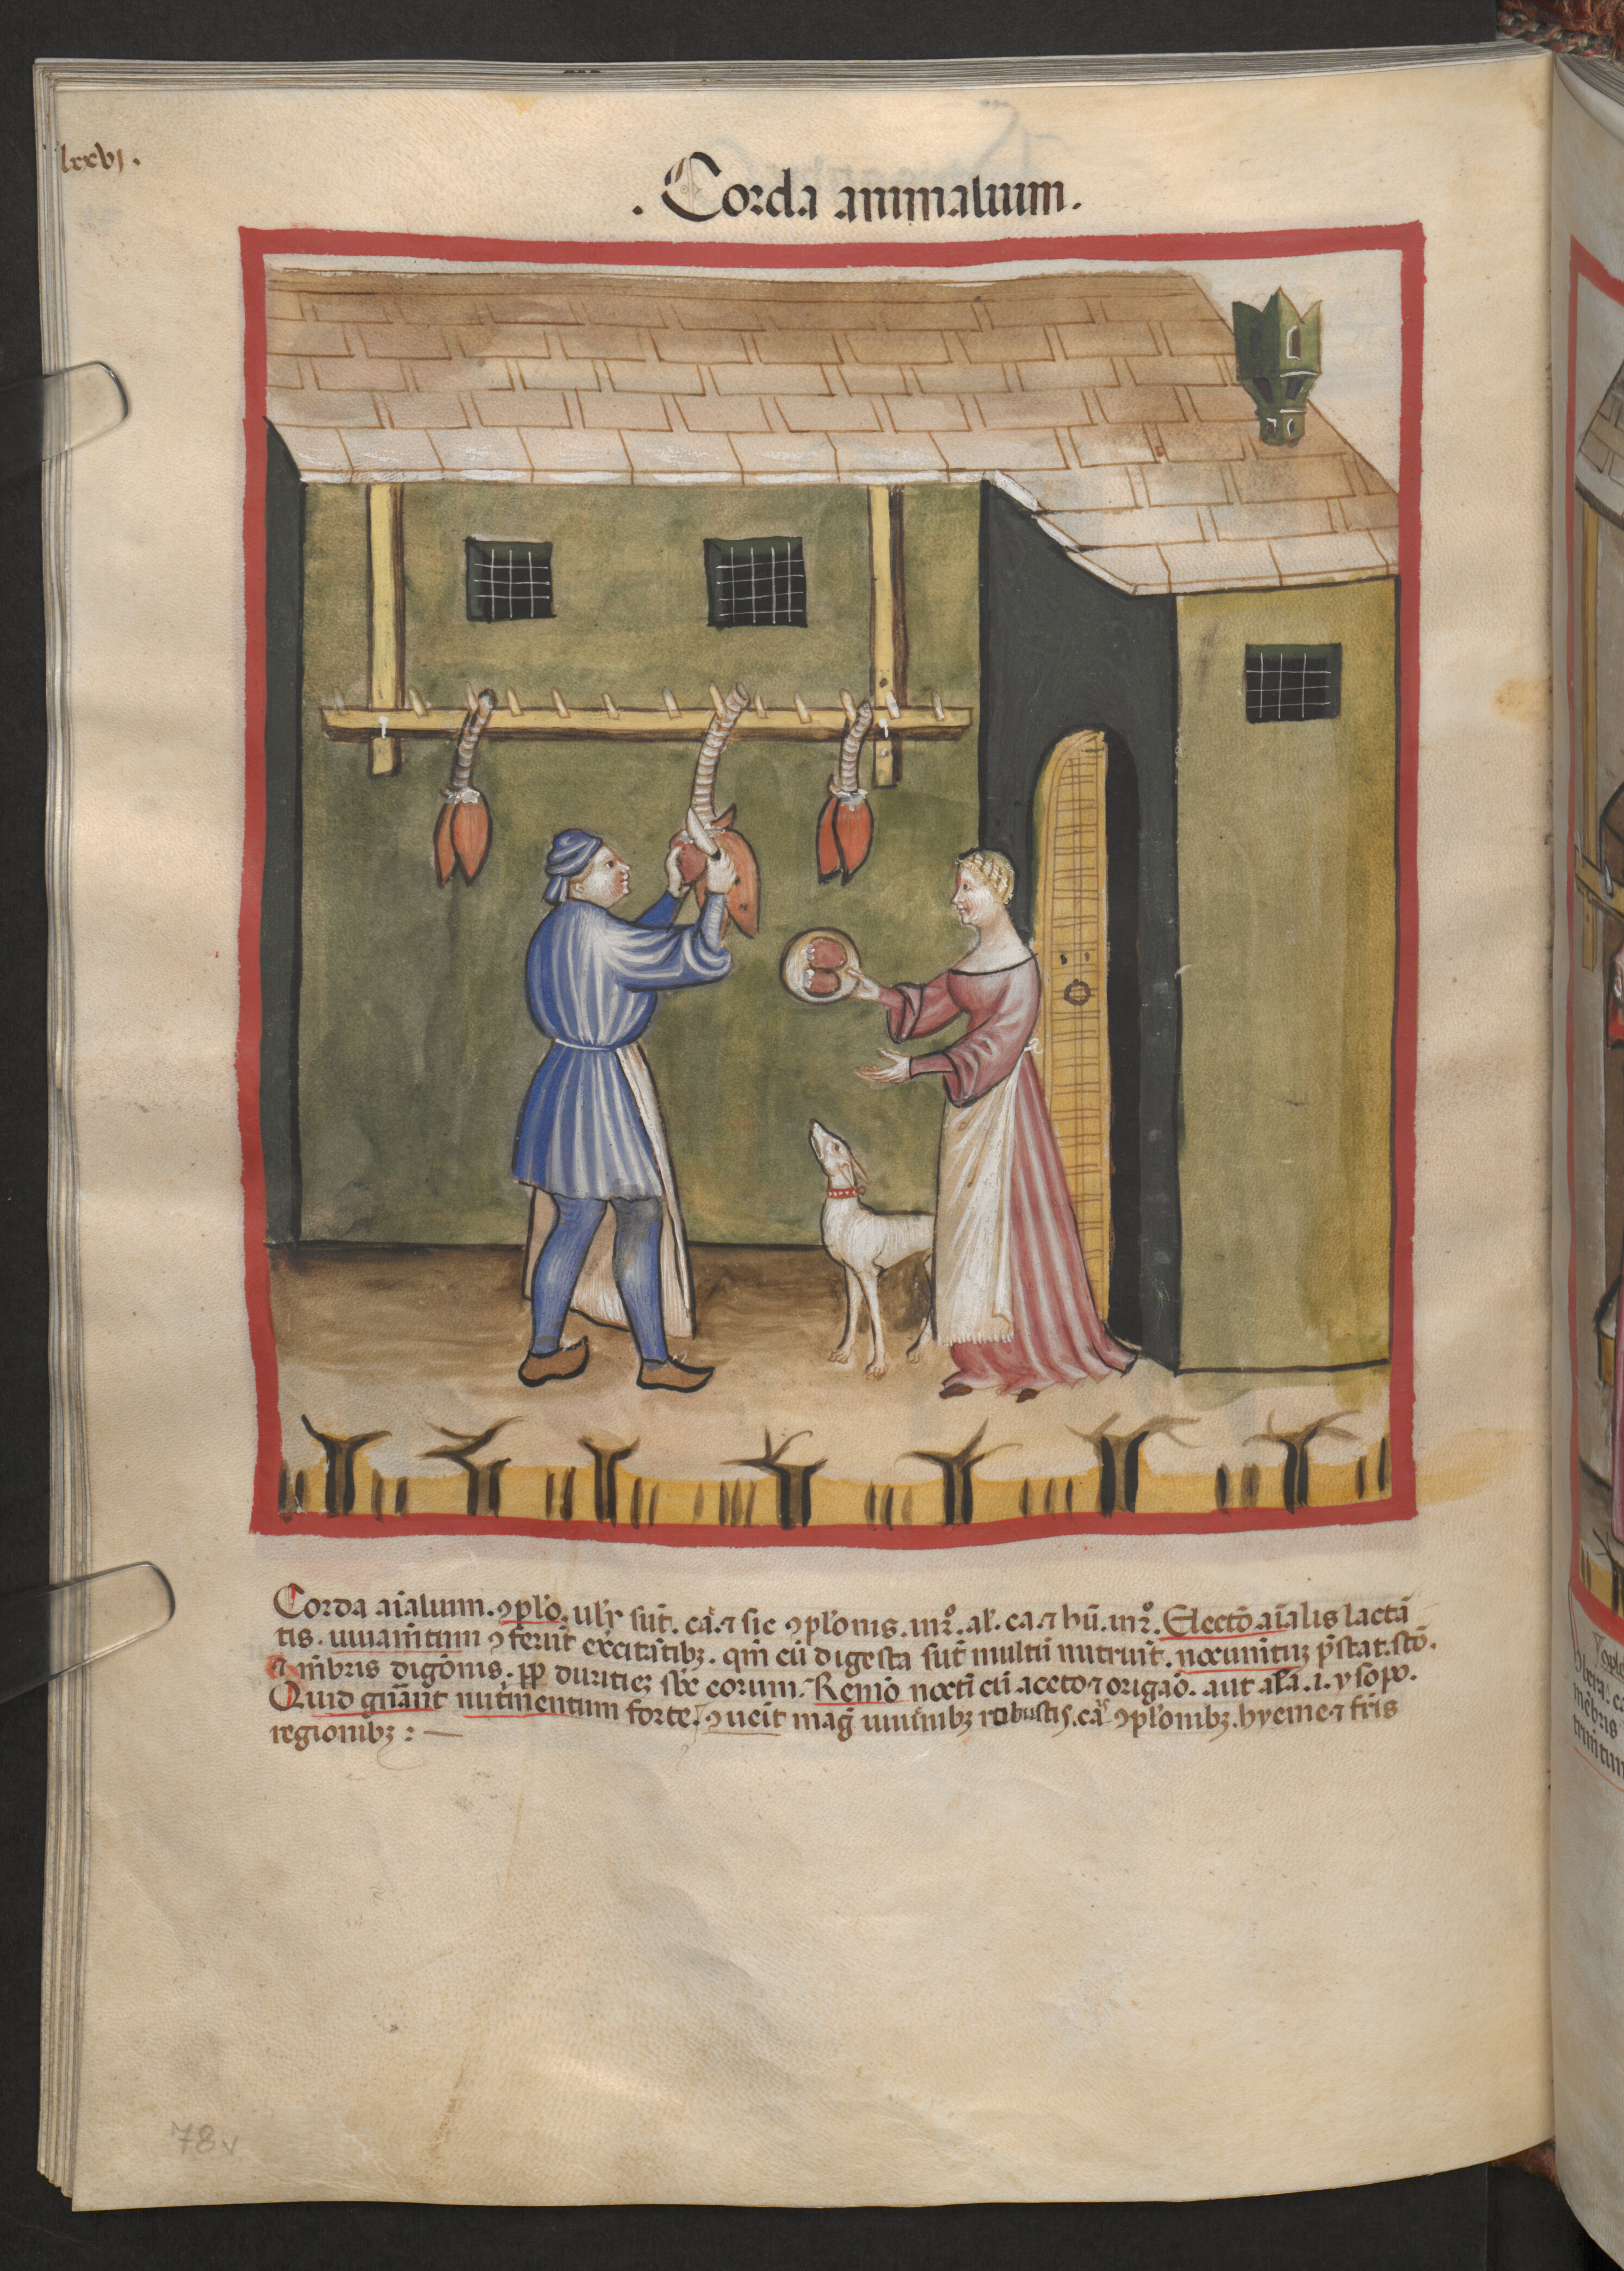
\includegraphics[width=0.45\textwidth]{Figures/Tacuinum_Sanitatis_p79L.png}
	\caption{\citep[page 79 Left]{TacSan}}
\end{figure}

\begin{figure}[!htb]
	\centering
	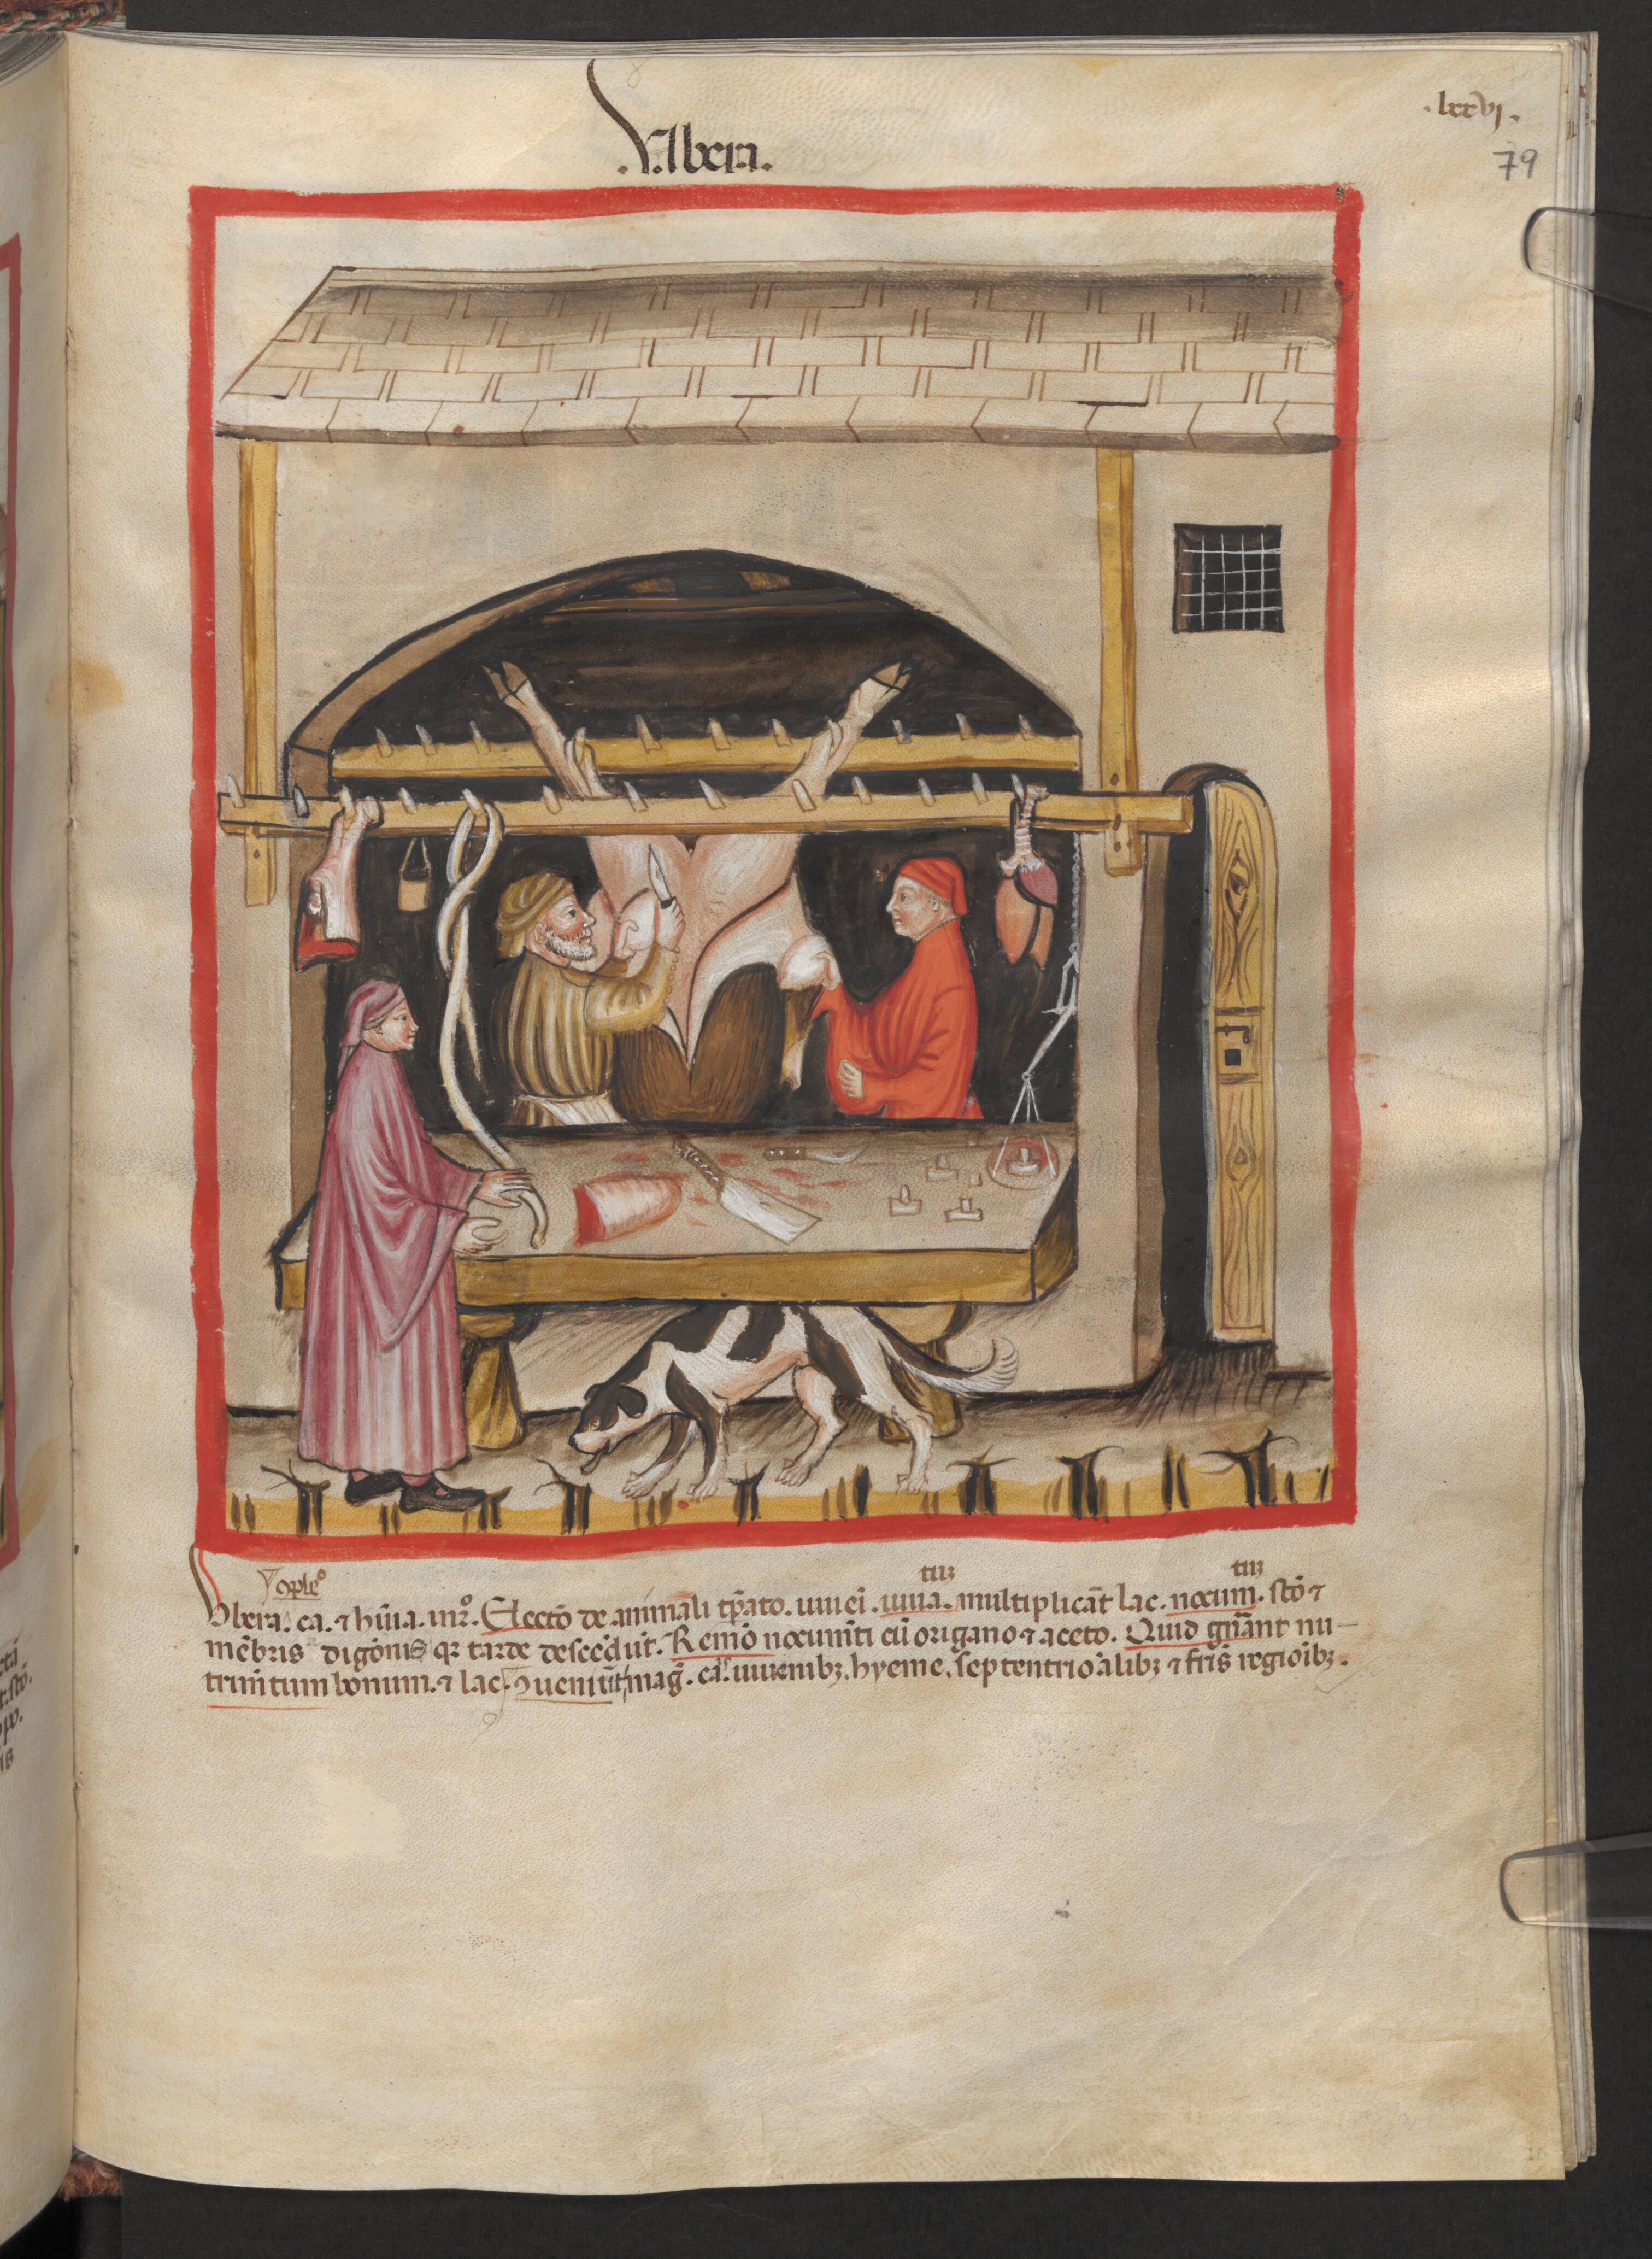
\includegraphics[width=0.45\textwidth]{Figures/Tacuinum_Sanitatis_p79R.png}
	\caption{\citep[page 79 Right]{TacSan}}
\end{figure}

\begin{figure}[!htb]
	\centering
	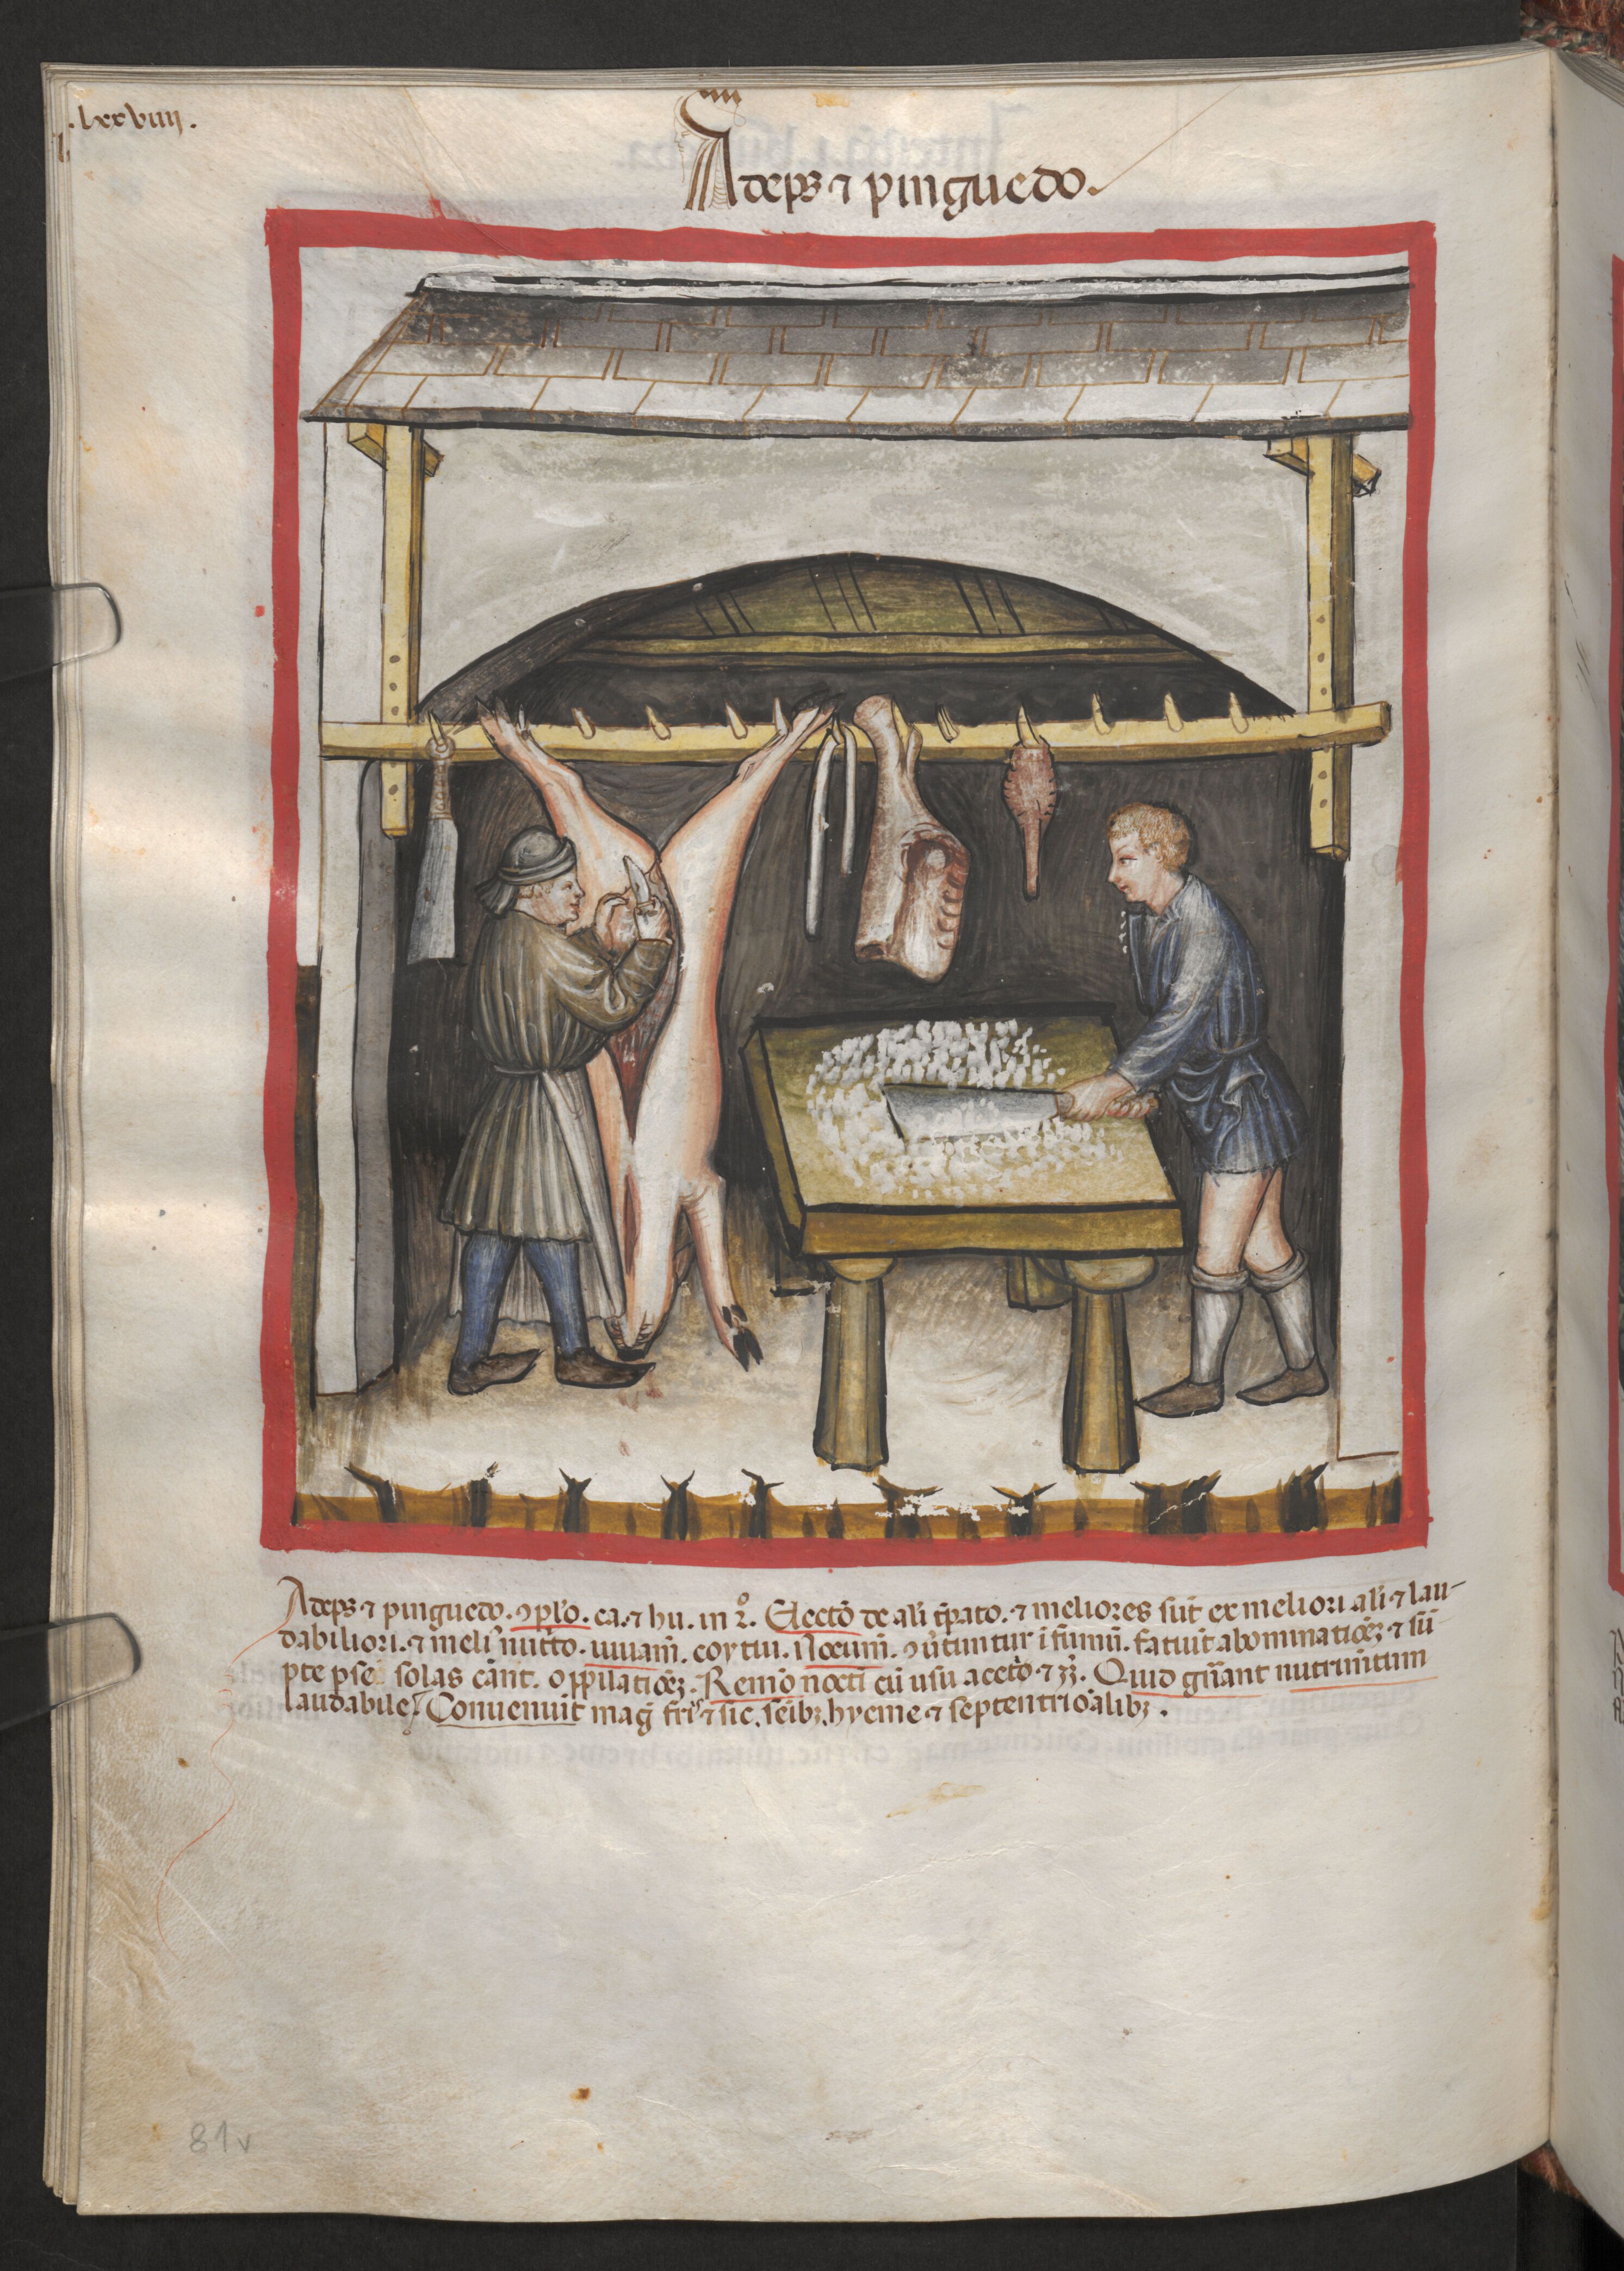
\includegraphics[width=0.45\textwidth]{Figures/Tacuinum_Sanitatis_p82L.png}
	\caption{\citep[page 82 Left]{TacSan}}
\end{figure}

\begin{figure}[!htb]
	\centering
	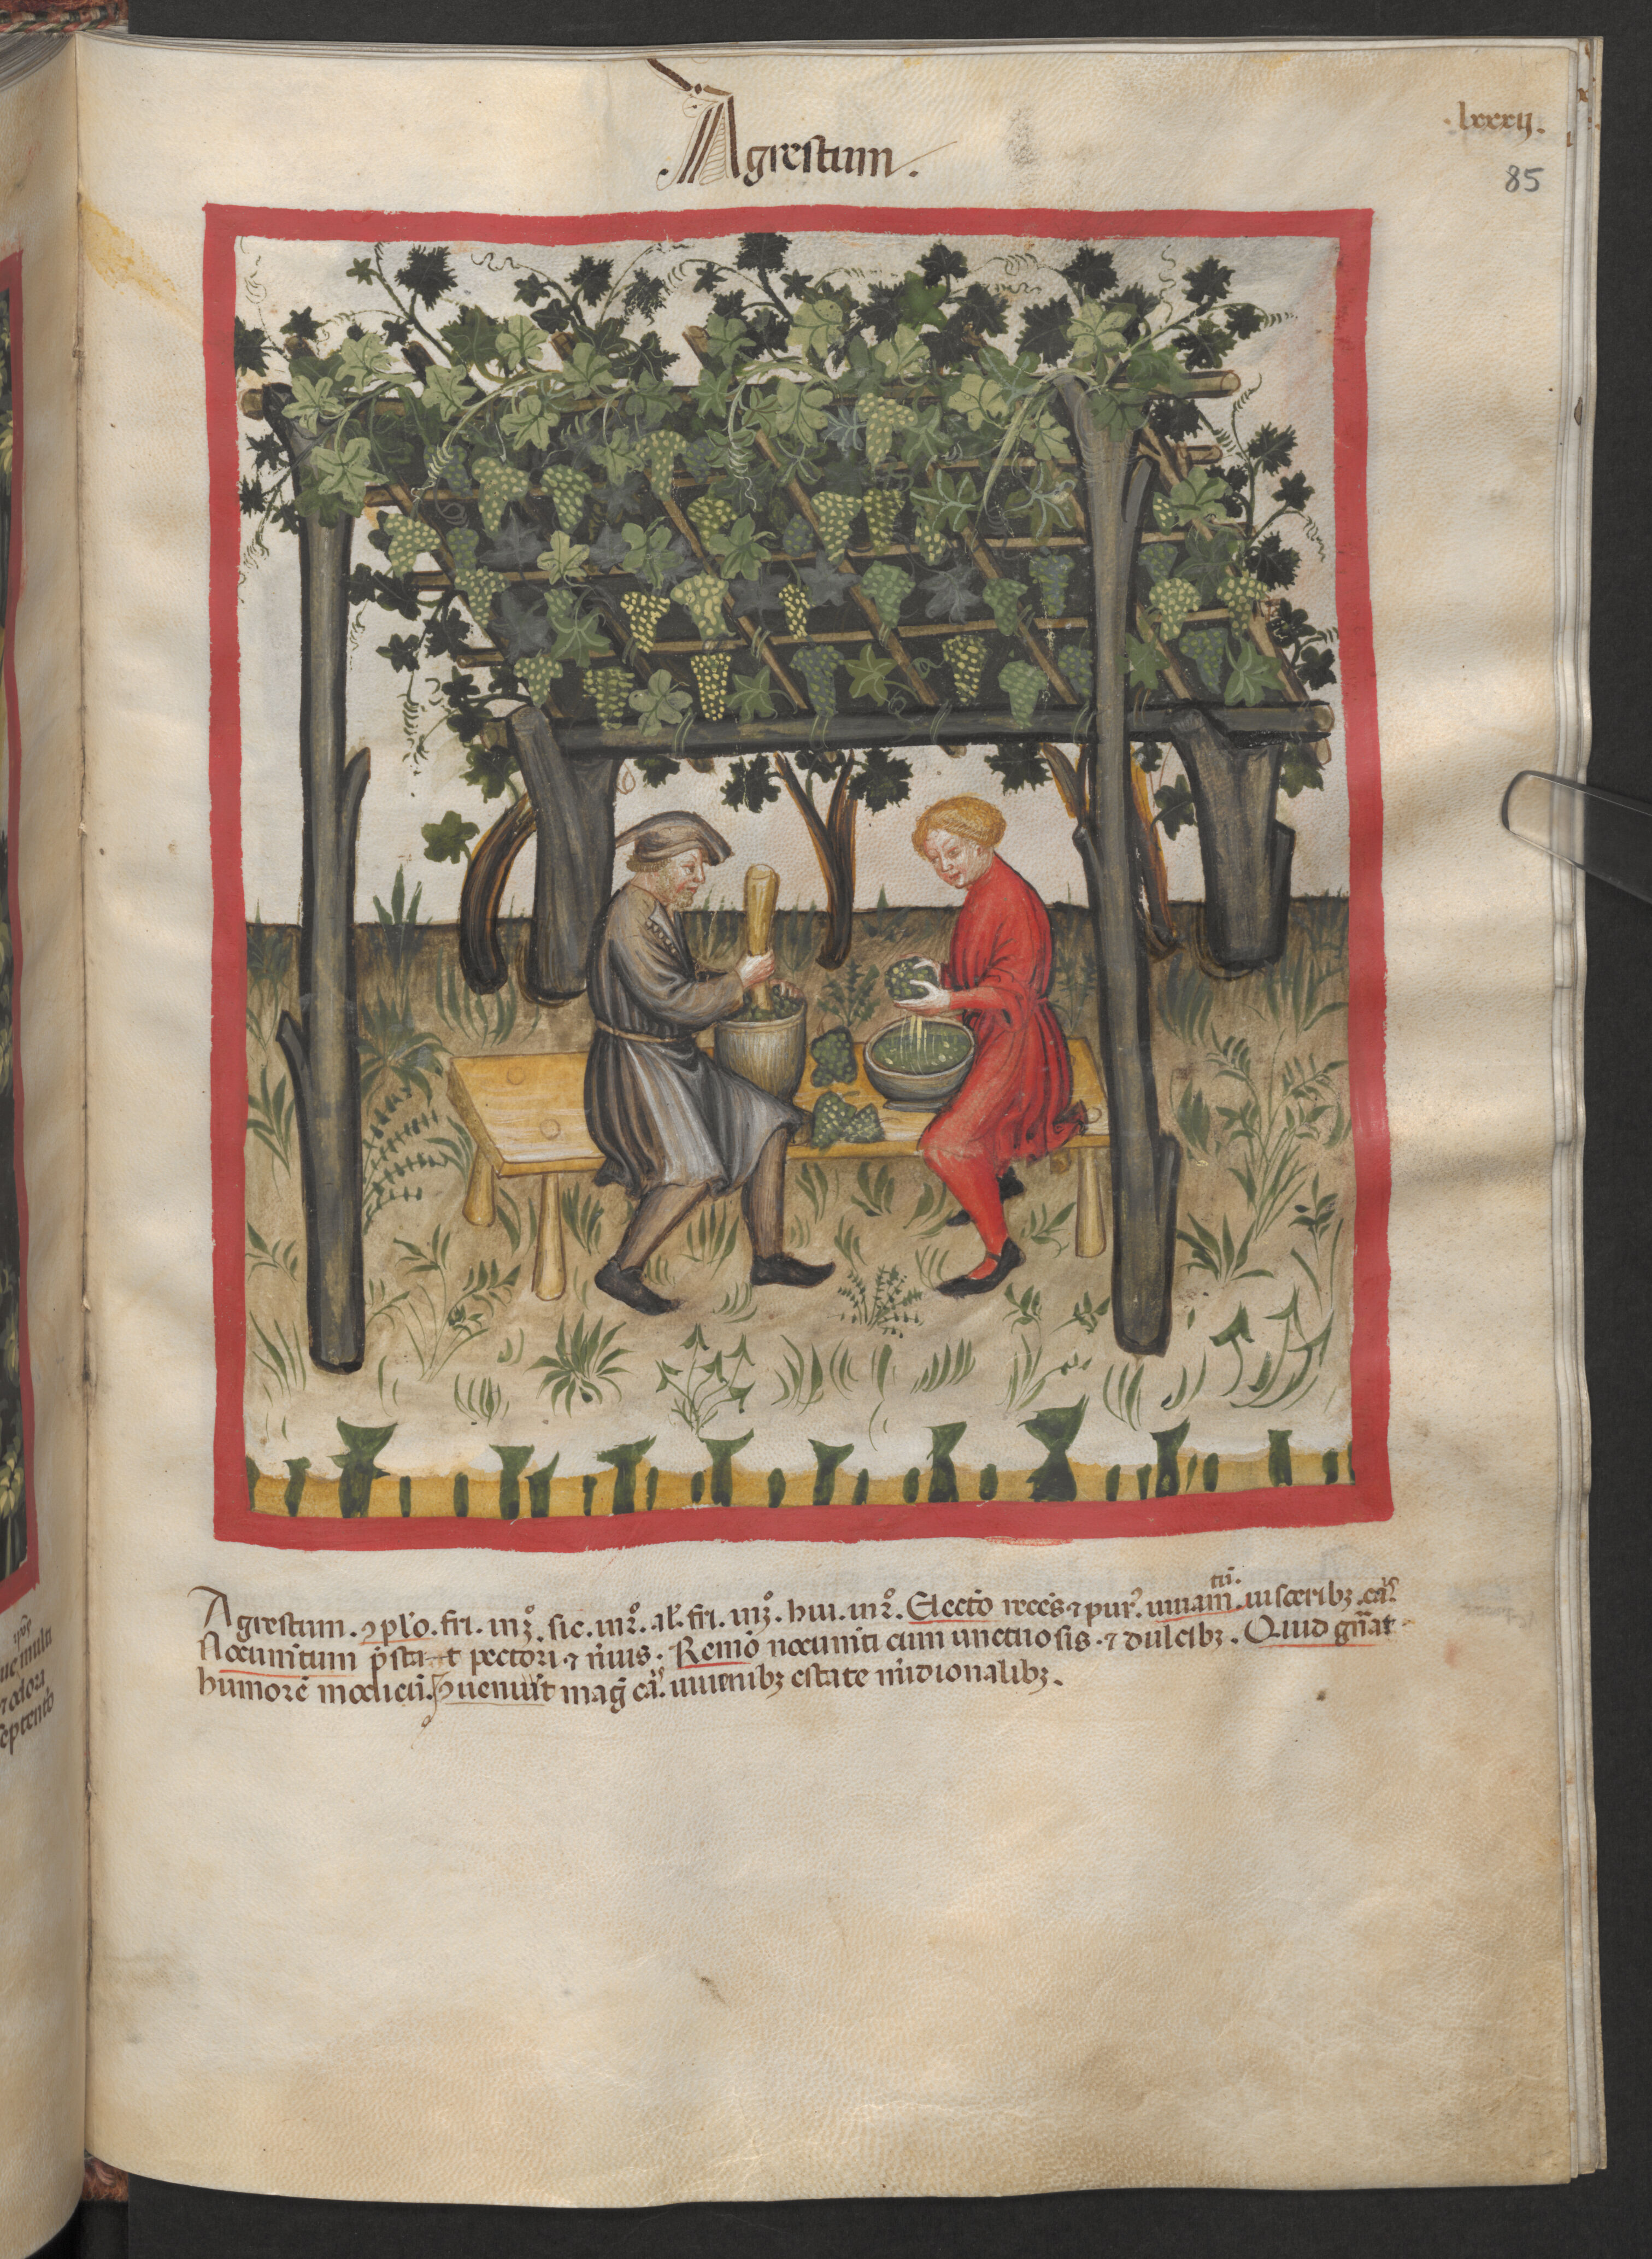
\includegraphics[width=0.45\textwidth]{Figures/Tacuinum_Sanitatis_p85R.png}
	\caption{\citep[page 85 Right]{TacSan}}
\end{figure}

\end{document}